\documentclass[review]{elsarticle}

\usepackage{geometry}
 \geometry{
 a4paper,
 left=30mm,
 right=30mm,
 top=10mm,
 bottom=10mm
 }

\usepackage{graphicx}
\usepackage{amsmath}

\usepackage{subcaption}

\usepackage{amssymb}
\usepackage{array}

\usepackage{lineno,hyperref}
\modulolinenumbers[5]

%\usepackage{numcompress}\bibliographystyle{model3-num-names}

\usepackage{natbib}
%\usepackage[numbers, sort&compress]{natbib}
%\setcitestyle{author[oxford]year}
\bibliographystyle{elsarticle-num}

%\geometry{verbose,tmargin=30mm,bmargin=25mm,lmargin=25mm,rmargin=25mm}
%\newcommand{\templatefigures}[1]
{\noindent
\begin{minipage}{2cm}
\begin{center}
%\linespread{1}
%\begin{figure}
  \centering
	\vspace{-1cm}
  
\includegraphics[height = 63px]{ISI2019only_with_date_small.pdf}\\
    %\label{matrix}
%\end{figure}
\end{center}
\end{minipage}
%
\quad
%
\begin{minipage}{12cm}
\hspace*{6.8cm}
\end{minipage}
%
\quad
%
\begin{minipage}{2cm}
\begin{center}
%\linespread{1}
\vspace{-0.9cm}

\includegraphics[scale=0.4]{imag2.jpg}\\
\end{center}

\end{minipage}

\vskip0.2cm
}


%\pagestyle{empty}
\begin{document}
%\templatefigures{}




% Model ensembles with different response variables for base and meta models:



% Spatial and Spatio-temporal Epidemiology
% Special issue: Disease Surveillance and Infectious disease Modeling


\begin{frontmatter}

\title{Supporting information: Improving disaggregation models of malaria incidence by ensembling non-linear models of prevalence}

\author[oxford]{Tim C. D. Lucas\corref{mycorrespondingauthor}}
\cortext[mycorrespondingauthor]{Corresponding author}
\ead{timcdlucas@gmail.com}
\author[oxford]{Anita K. Nandi}
\author[oxford]{Suzanne H. Keddie}
%\author[oxford]{Katherine A. Twohig}
\author[oxford]{Elisabeth G. Chestnutt}
\author[oxford]{Rosalind E. Howes}
%\author[oxford]{Michele Nguyen}
\author[oxford]{Susan F. Rumisha}
\author[oxford]{Rohan Arambepola}
\author[oxford,idm]{Amelia Bertozzi-Villa}
\author[oxford]{Andre Python}
\author[oxford]{Tasmin L. Symons}
\author[oxford]{Justin J. Millar}
\author[oxford]{Punam Amratia}
\author[oxford]{Penelope Hancock}
\author[oxford]{Katherine E. Battle}
\author[oxford]{Ewan Cameron}
\author[oxford,telethon,curtin]{Peter W. Gething}
\author[oxford]{Daniel J. Weiss}



\address[oxford]{Malaria Atlas Project, Big Data Institute, University of Oxford, Oxford, UK}
\address[idm]{Institute for Disease Modeling, Bellevue, WA, USA}
\address[telethon]{Telethon Kids Institute, Perth Children’s Hospital, Perth, Australia}
\address[curtin]{Curtin University, Perth, Australia}



\end{frontmatter}

\clearpage
\tableofcontents


\clearpage
\section{Global dataset Machine Learning}

\clearpage
\subsection{Out-of-sample scatter plots}


\begin{figure}[h!]
  \centering
  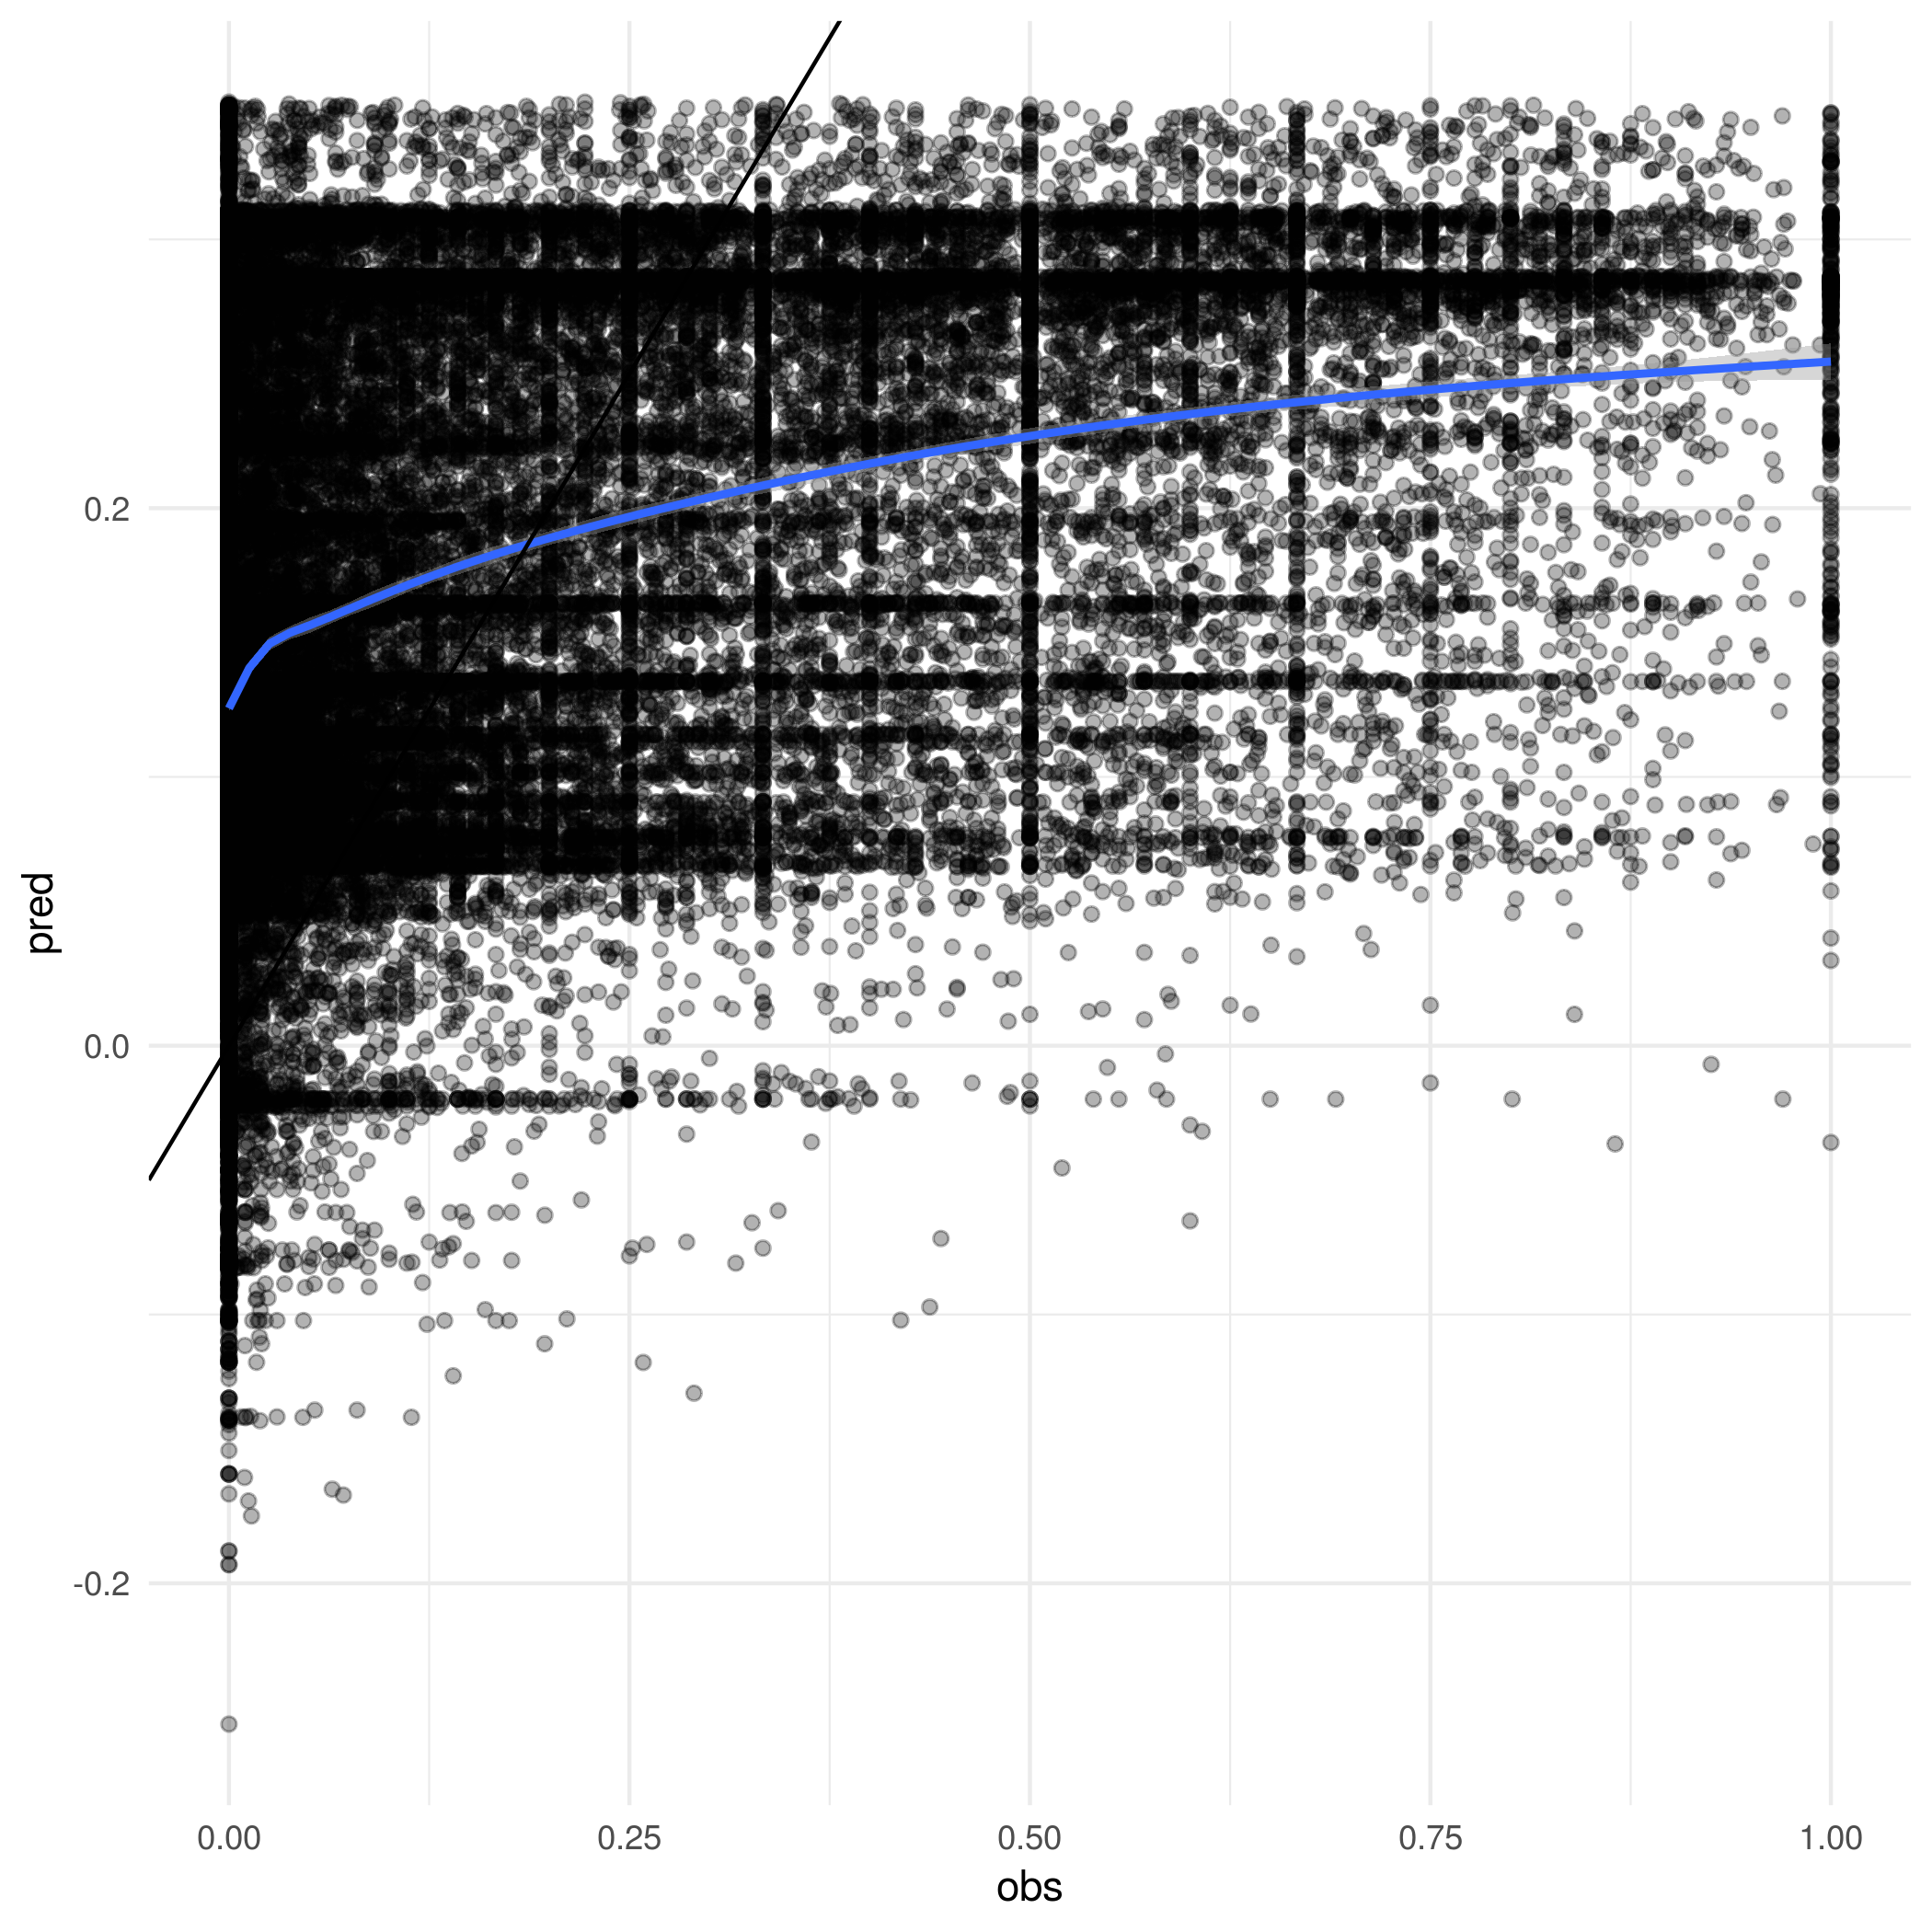
\includegraphics[width=0.6\textwidth]{figs/SI/nnet_obspred_global.png}
\caption{
  Scatter plot of predictions and held out observed data for the neural network trained on the global dataset.
}

\end{figure}



\begin{figure}[h!]
  \centering
  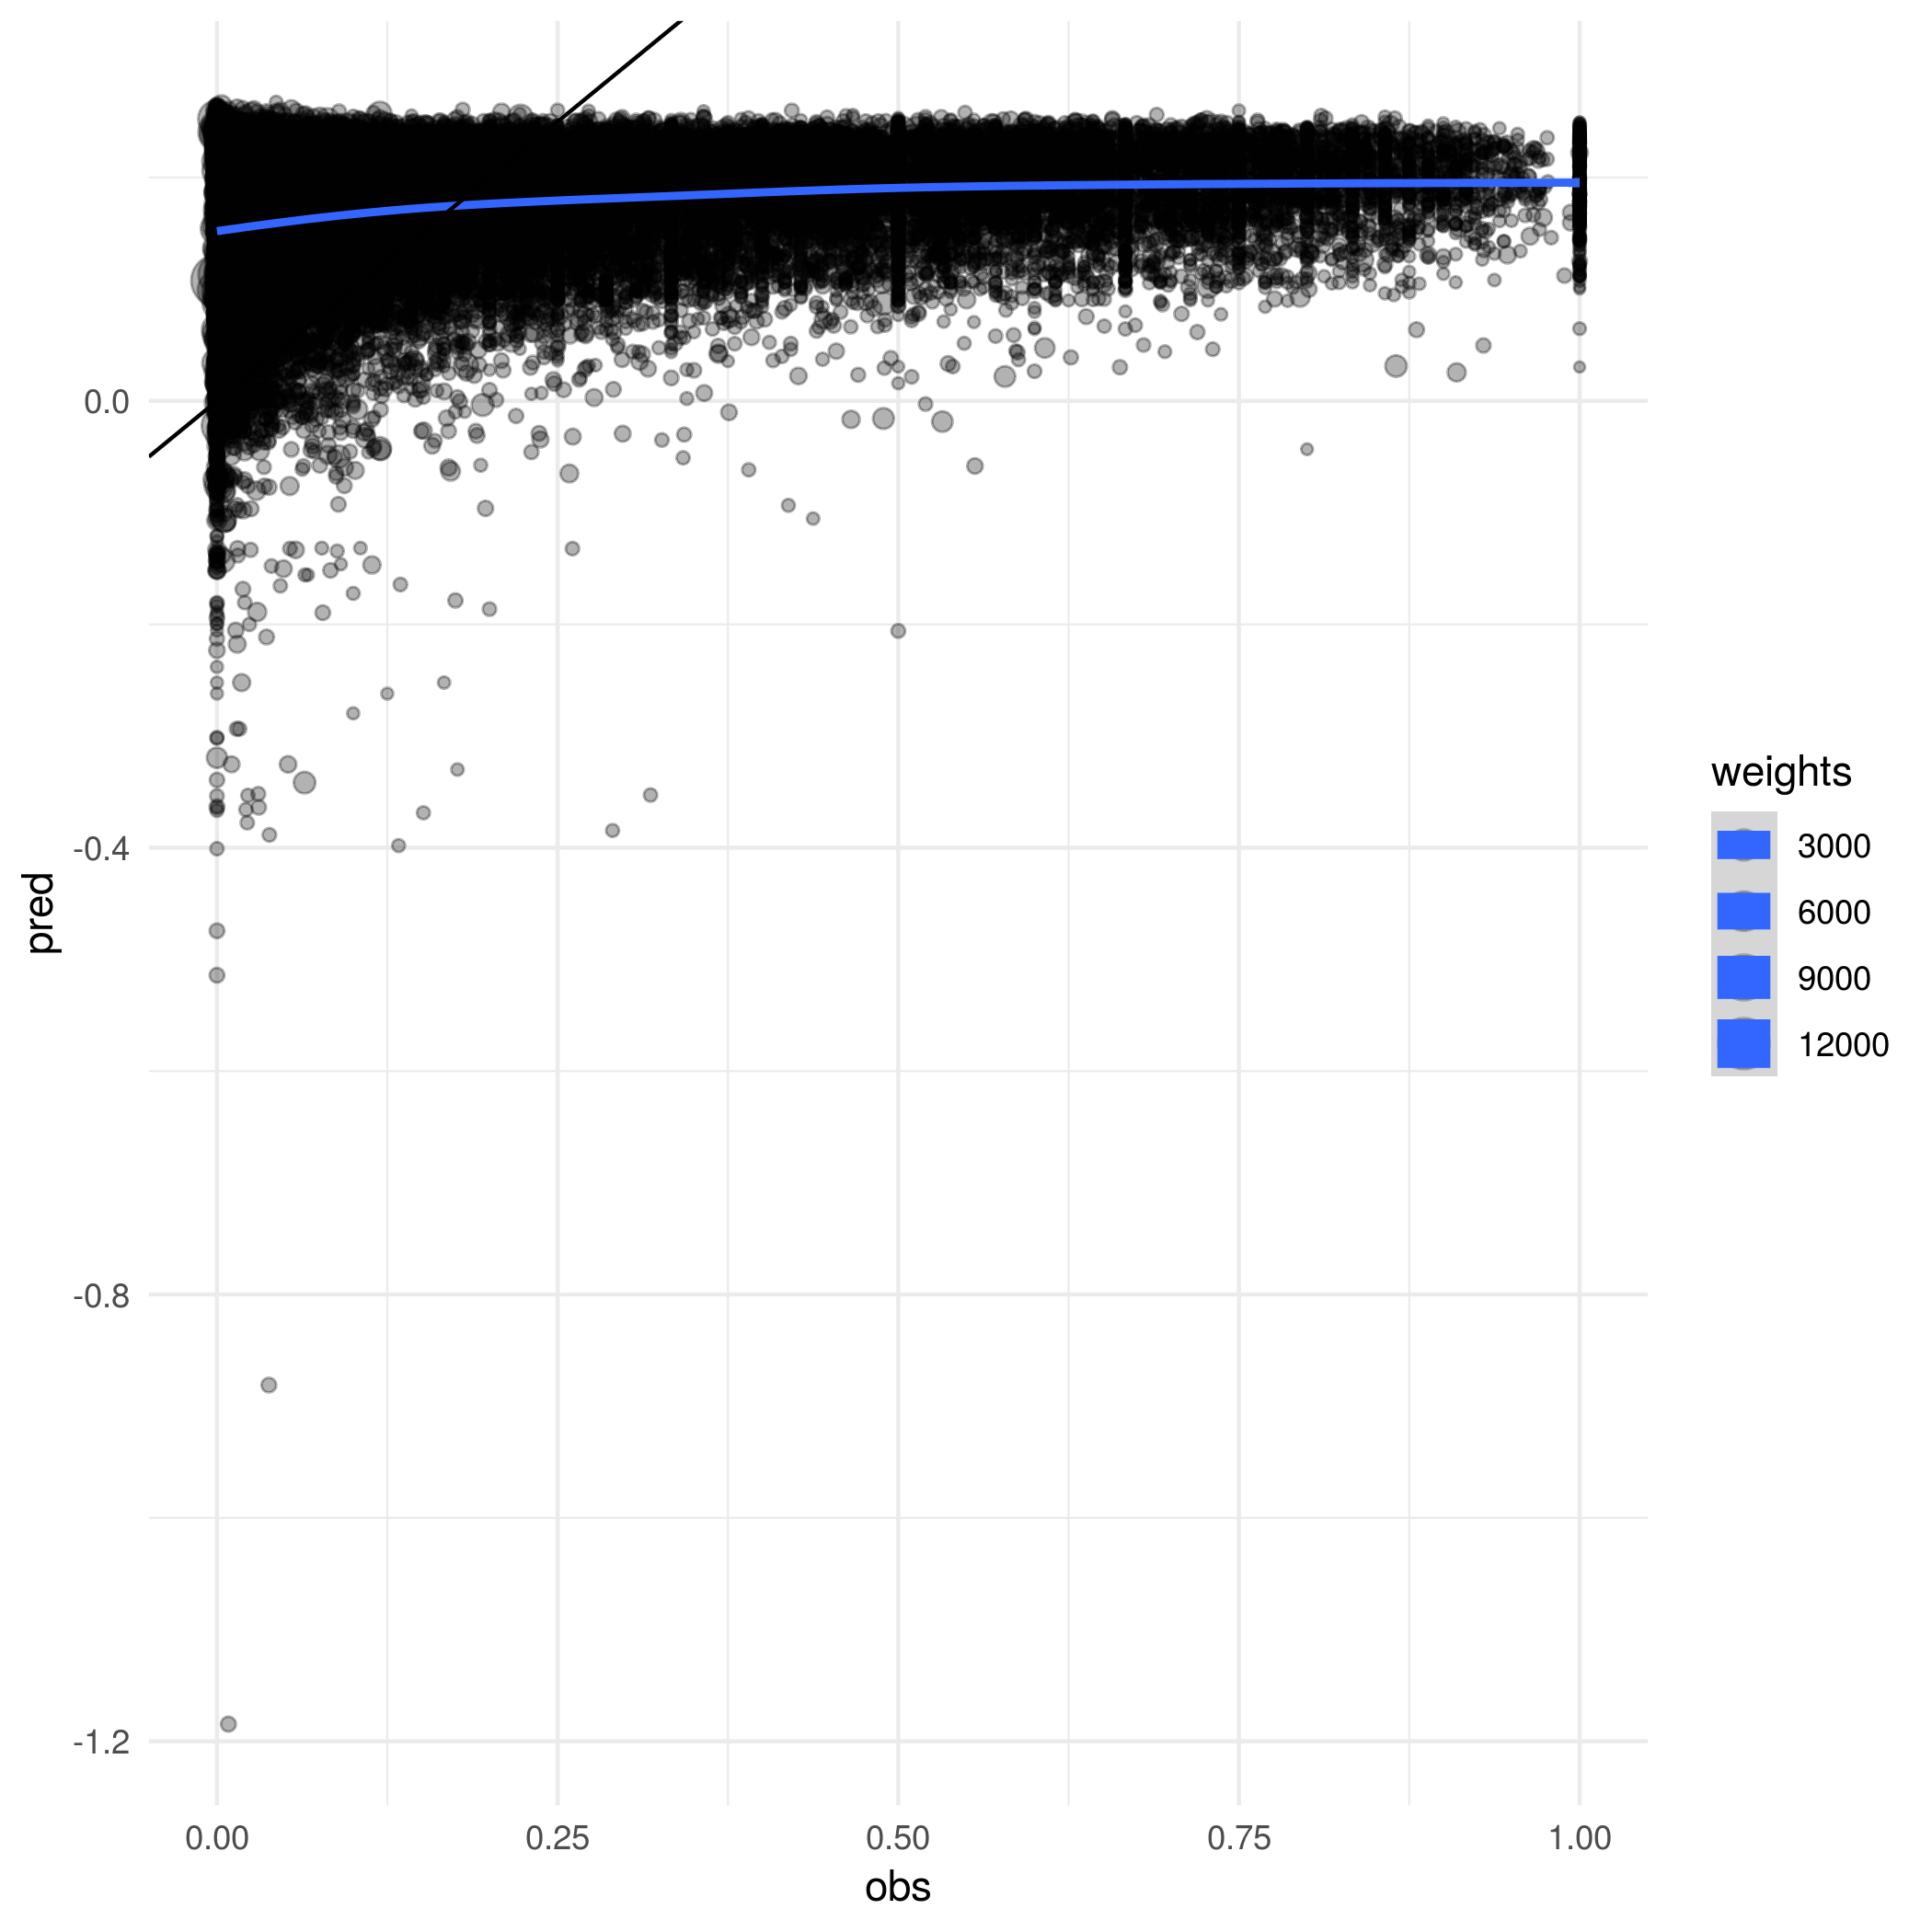
\includegraphics[width=0.6\textwidth]{figs/SI/enet_obspred_global.png}
\caption{
  Scatter plot of predictions and held out observed data for the elastic net trained on the global dataset.
}

\end{figure}


\begin{figure}[h!]
  \centering
  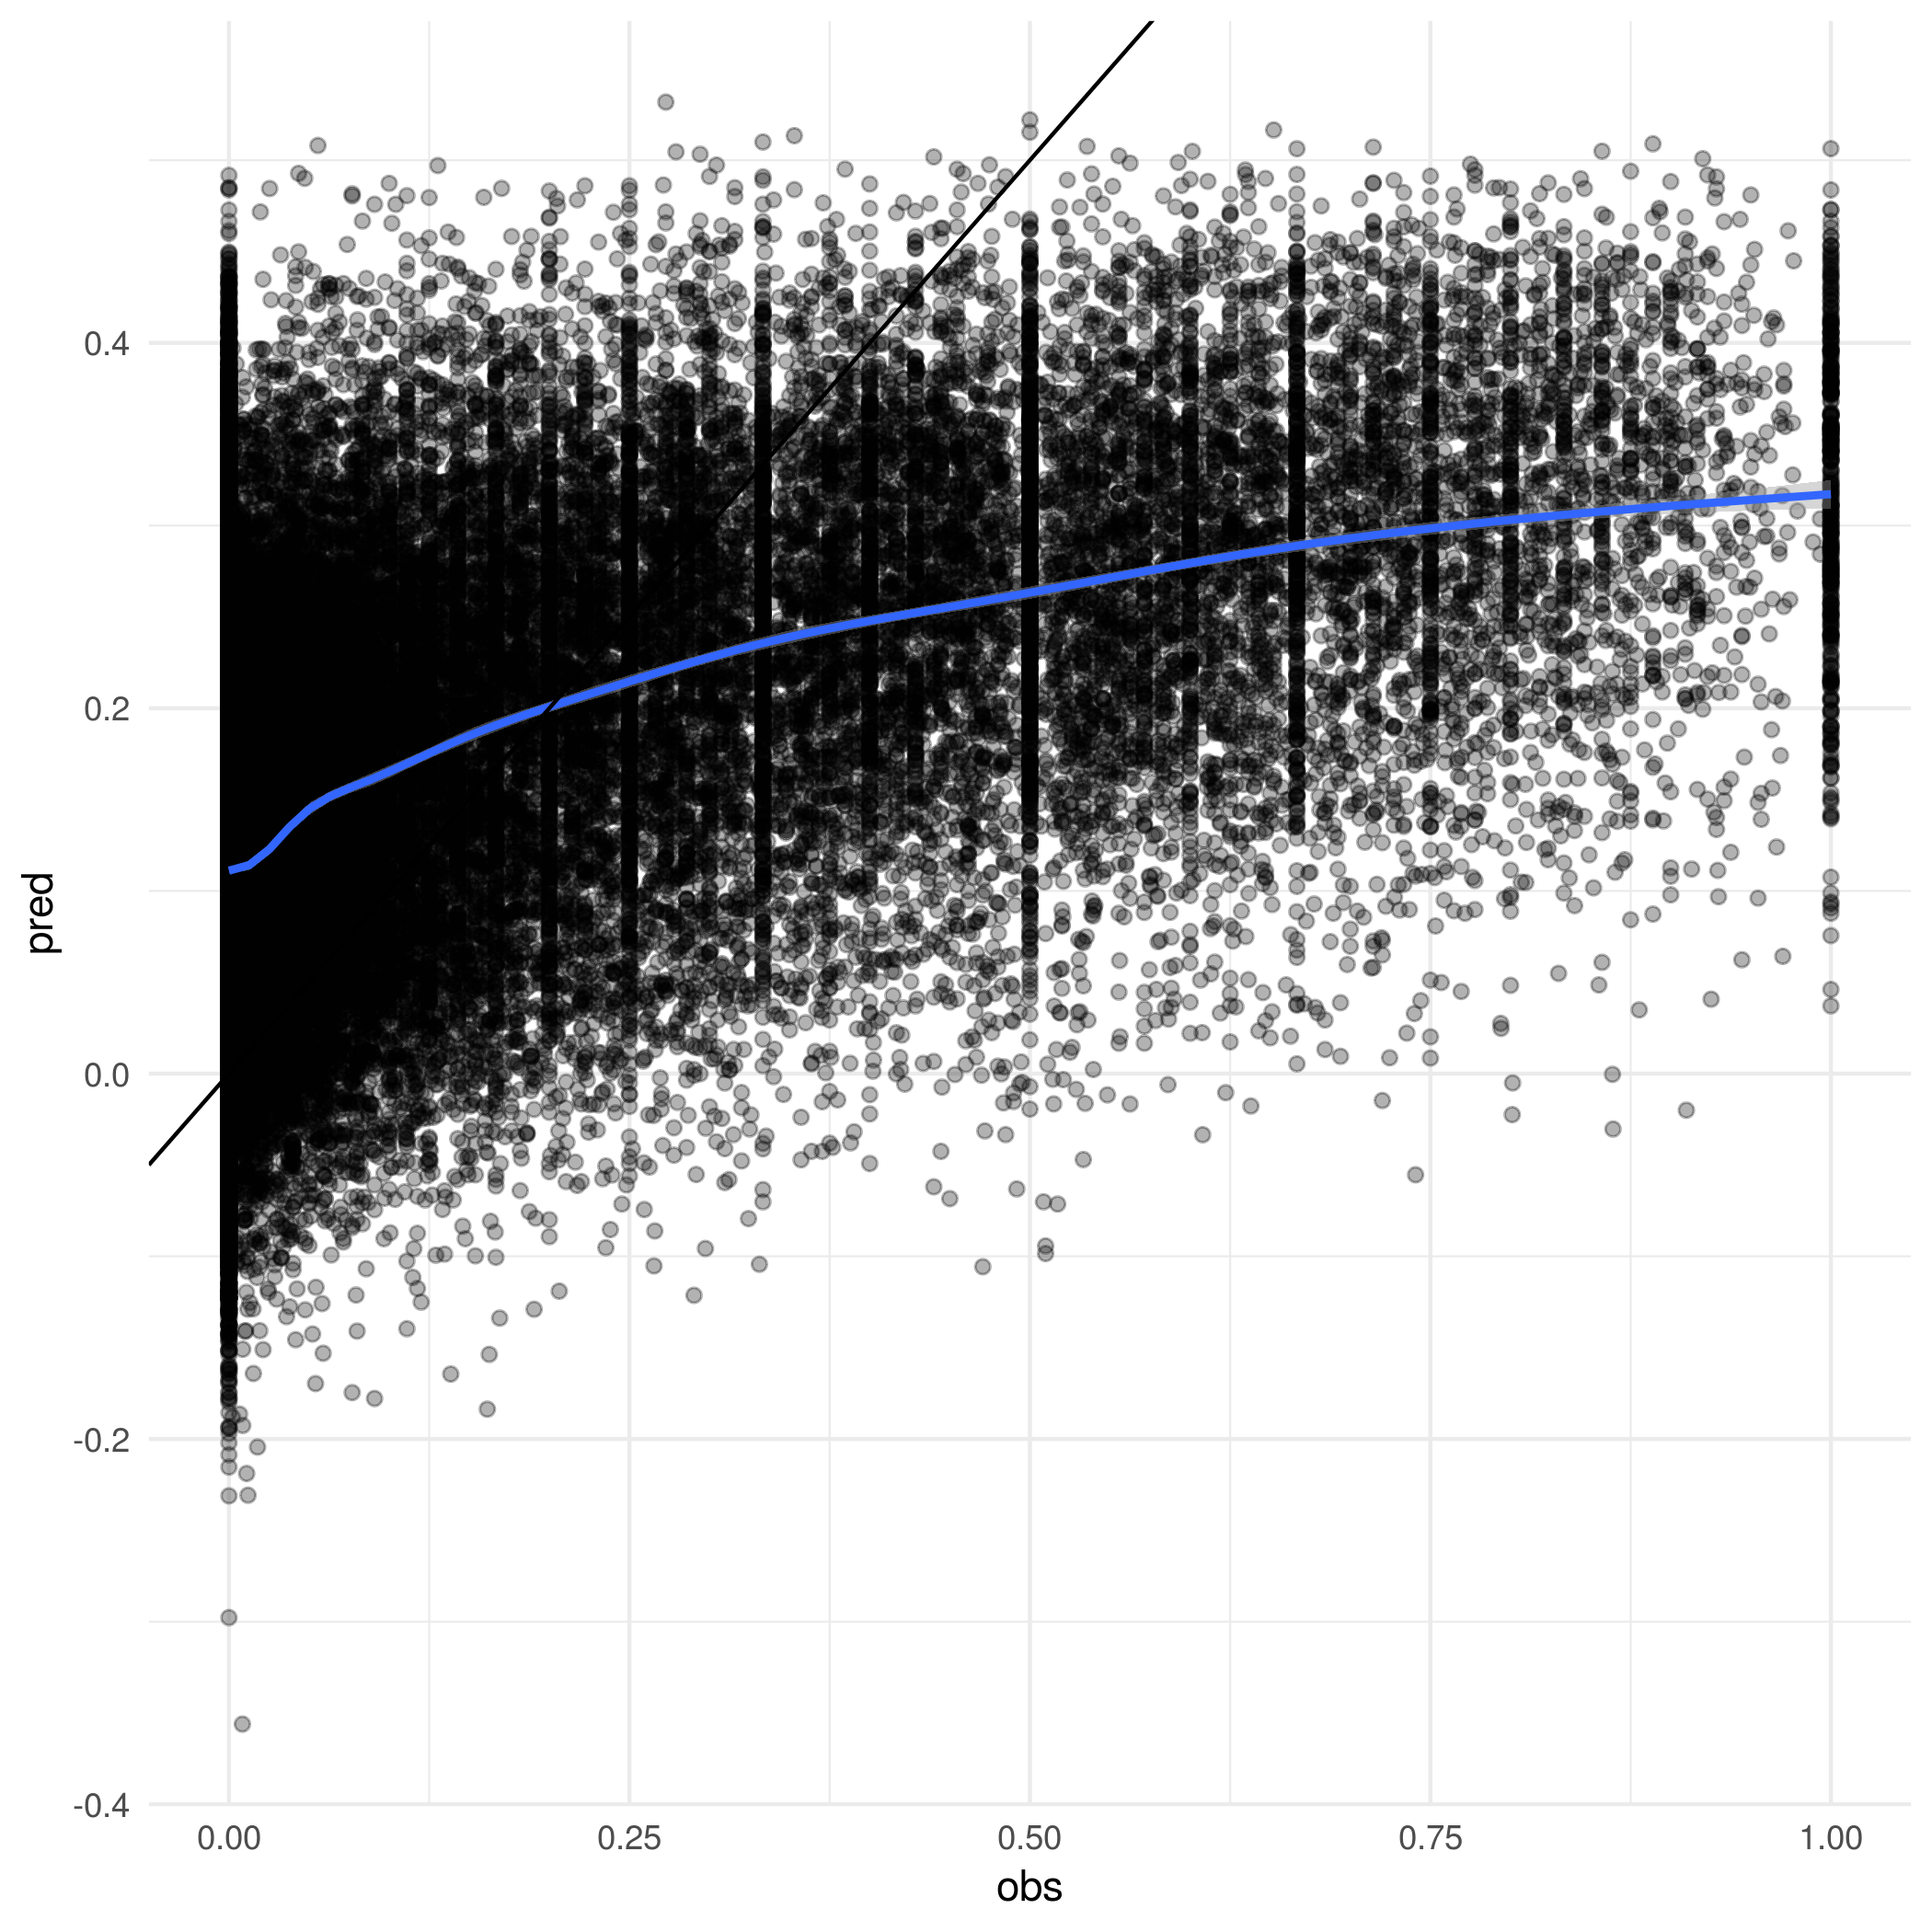
\includegraphics[width=0.6\textwidth]{figs/SI/ppr_obspred_global.png}
\caption{
  Scatter plot of predictions and held out observed data for the PPR trained on the global dataset.
}

\end{figure}


\begin{figure}[h!]
  \centering
  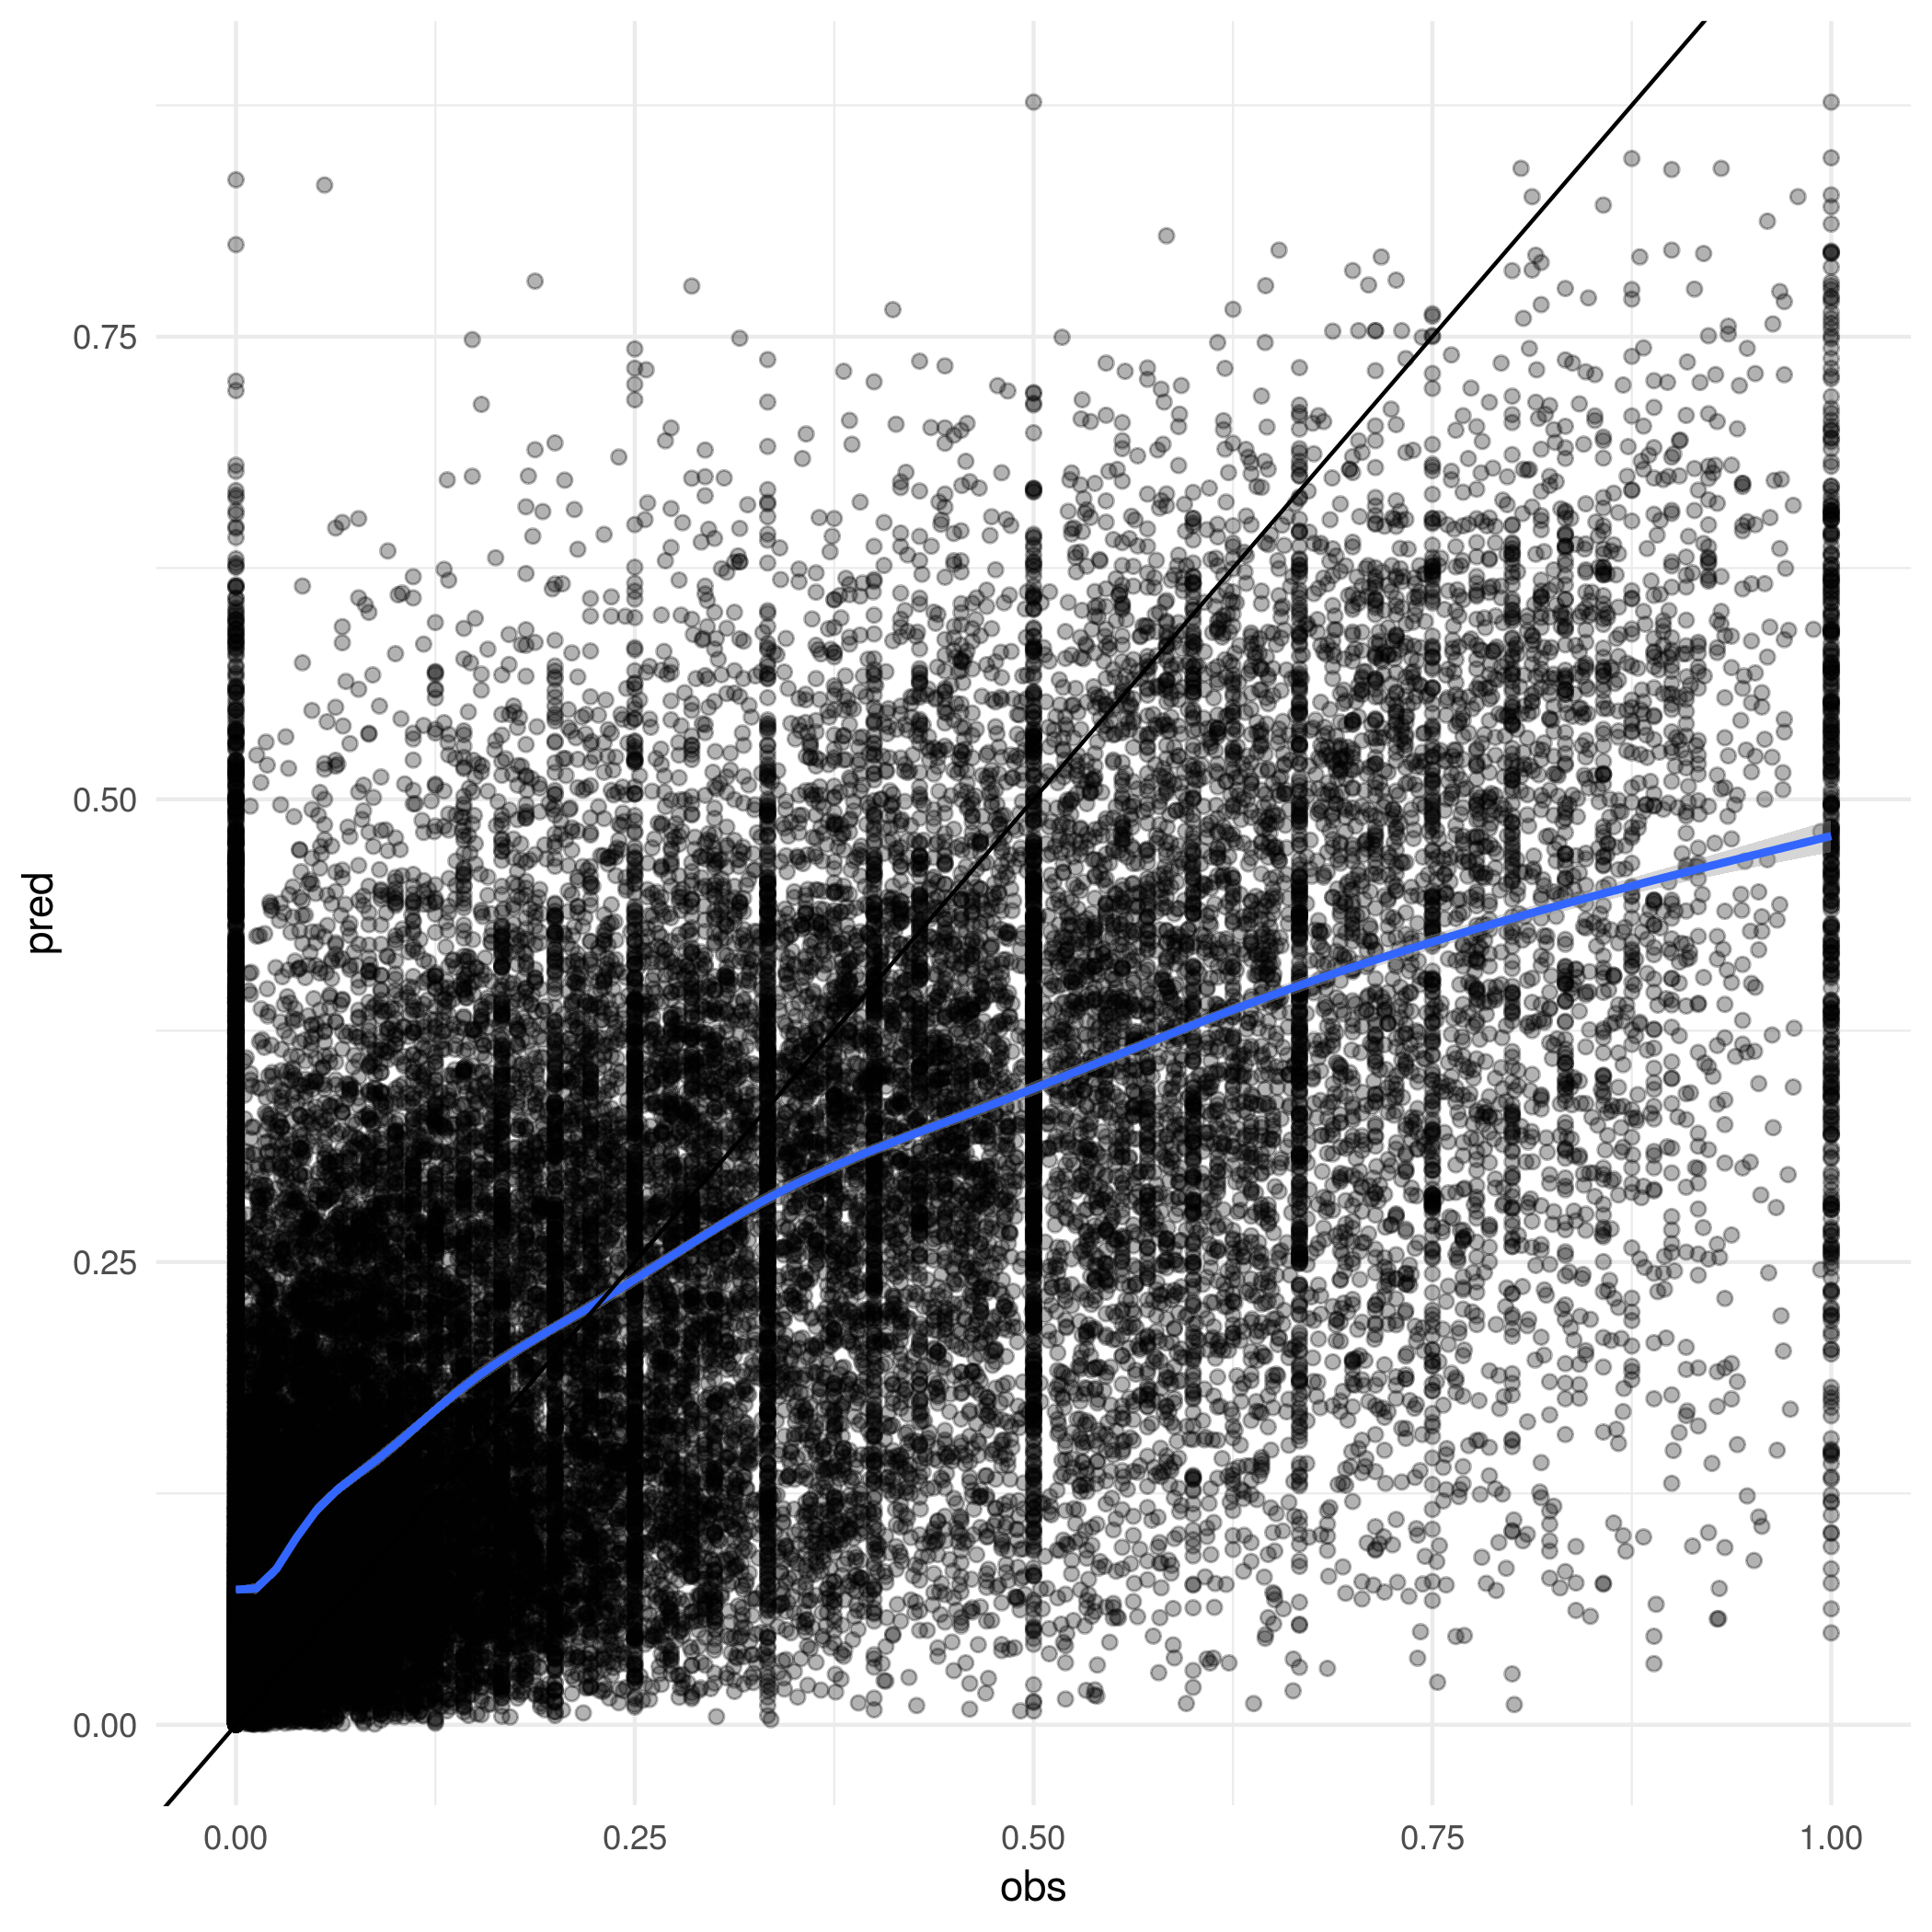
\includegraphics[width=0.6\textwidth]{figs/SI/ranger_obspred_global.png}
\caption{
  Scatter plot of predictions and held out observed data for the Random Forest trained on the global dataset.
}

\end{figure}


\begin{figure}[h!]
  \centering
  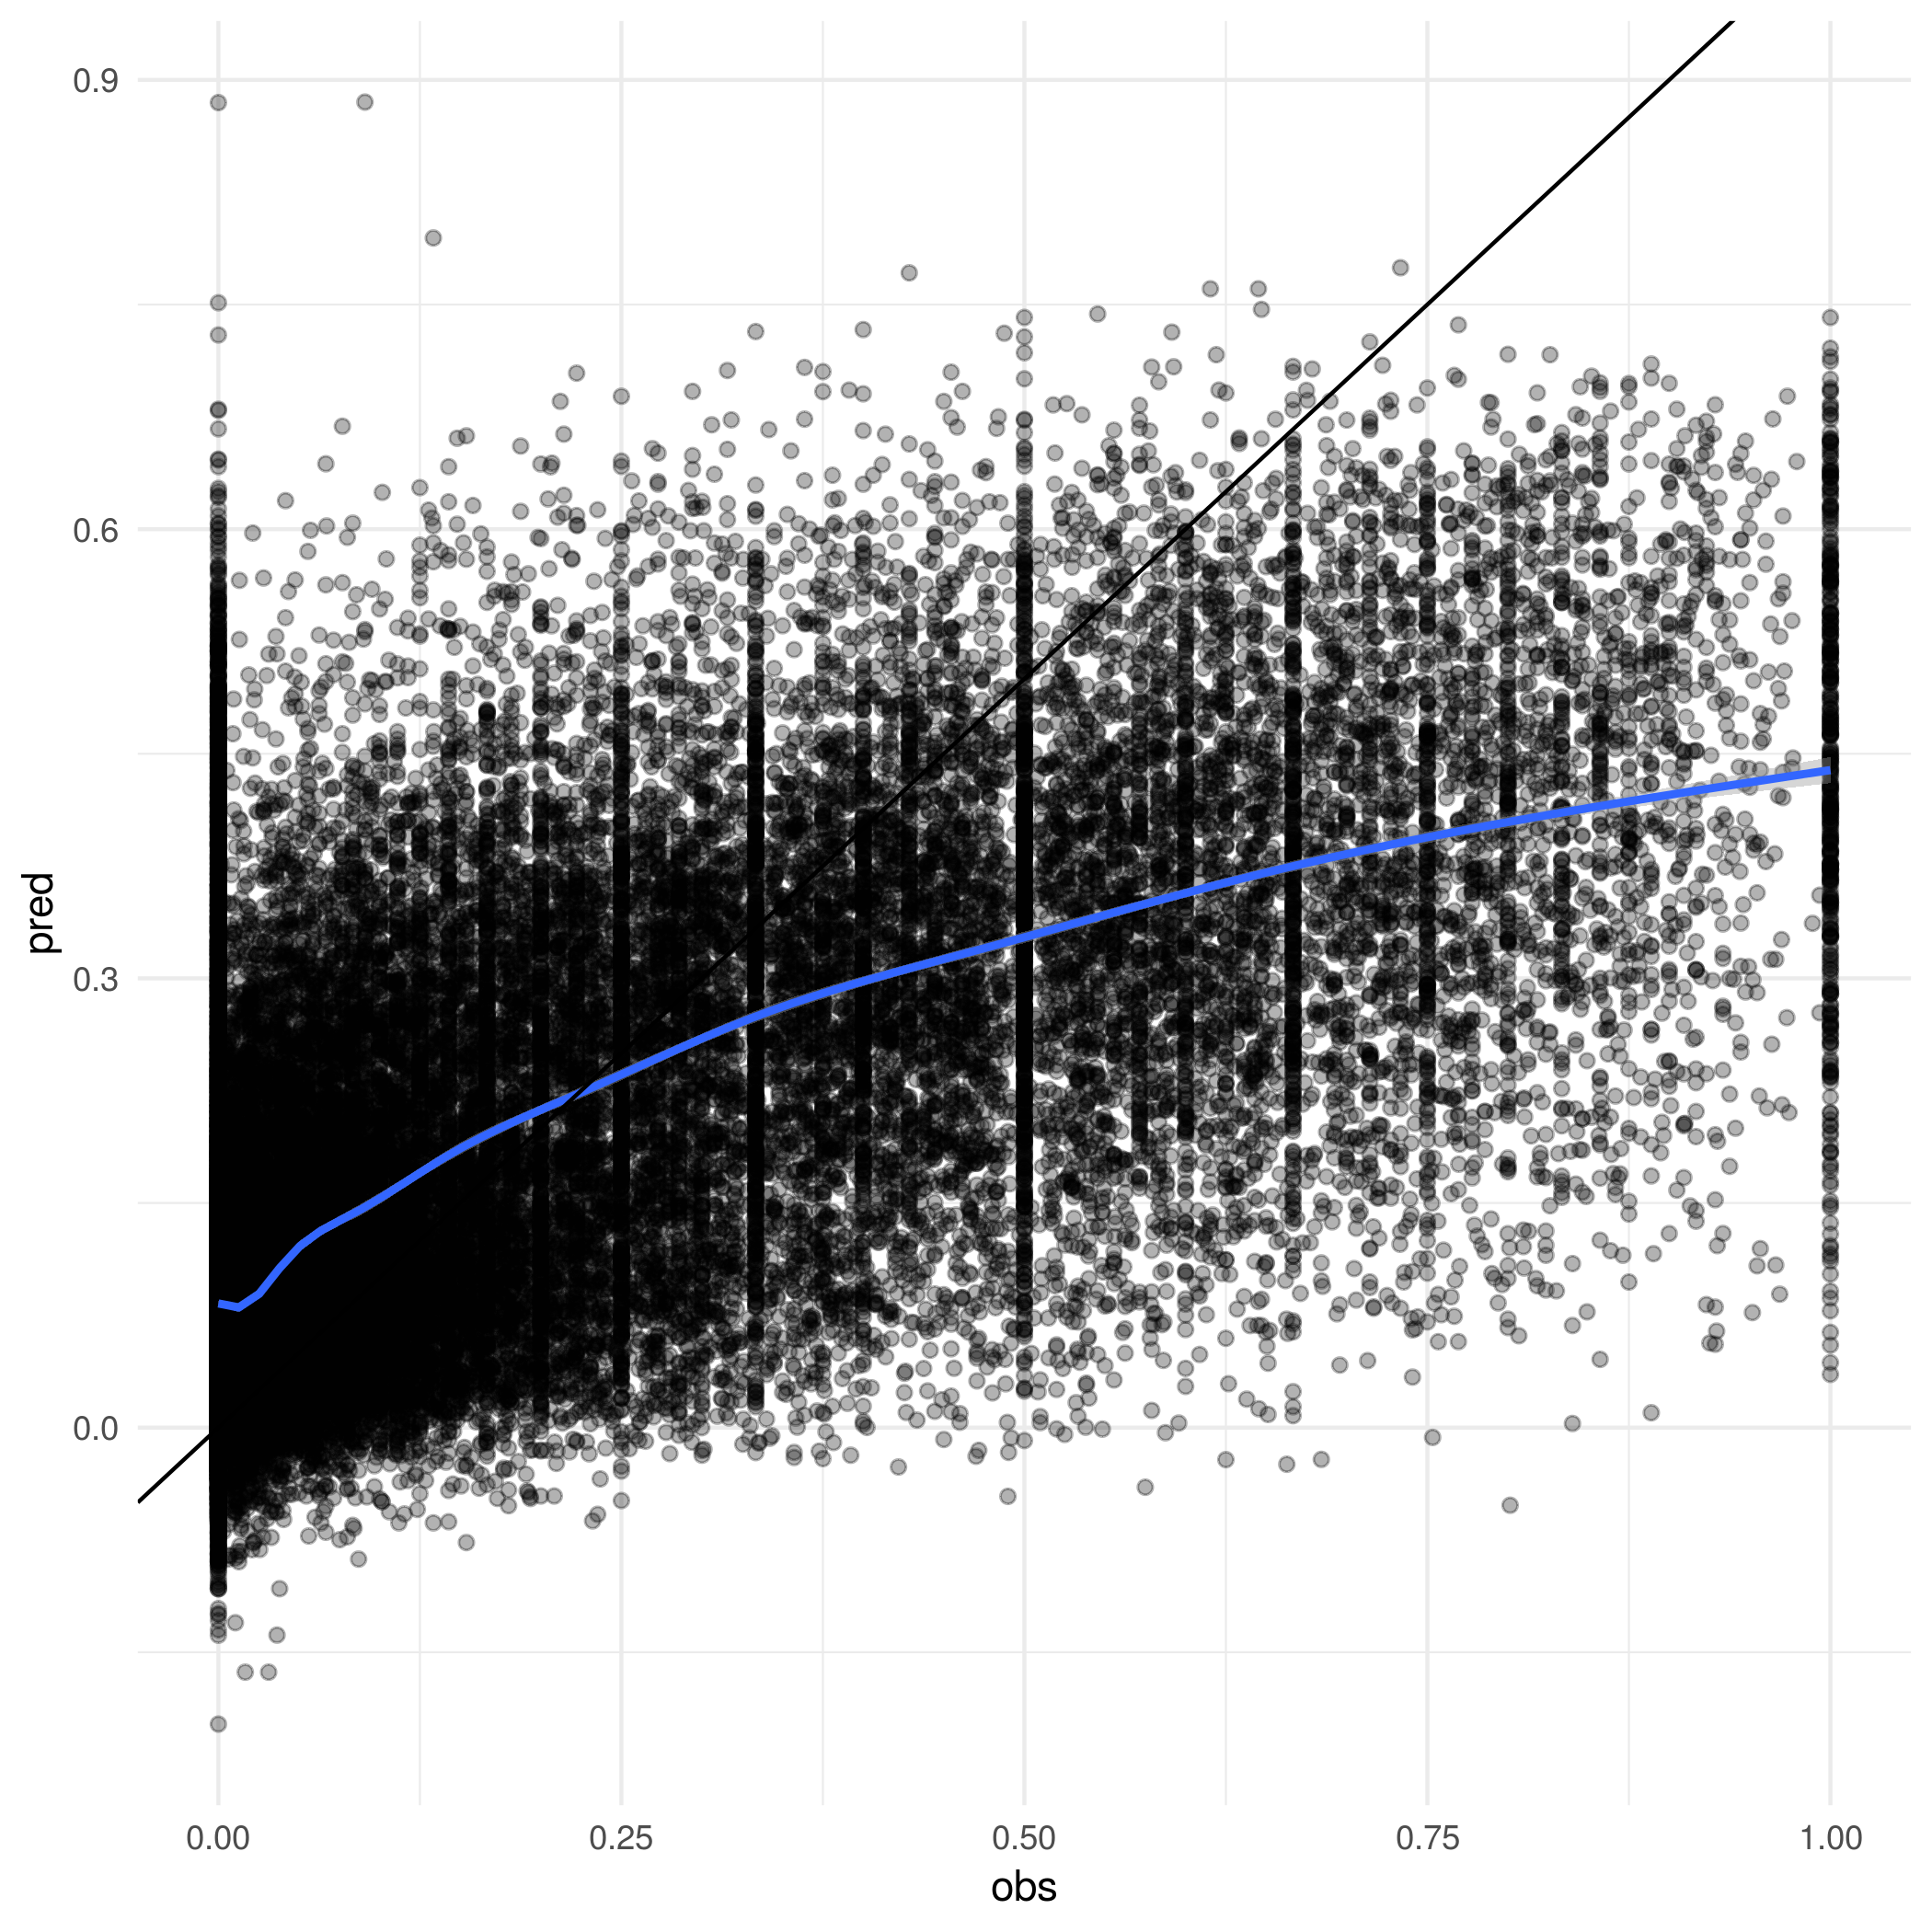
\includegraphics[width=0.6\textwidth]{figs/SI/gbm_obspred_global.png}
\caption{
  Scatter plot of predictions and held out observed data for the GBM trained on the global dataset.
}

\end{figure}


\clearpage
\subsection{Hyperparameter optimisation}

As ranger and GBM were tuned with random hyperparameter search, the plots become difficult and are not included.

\begin{figure}[h!]
  \centering
  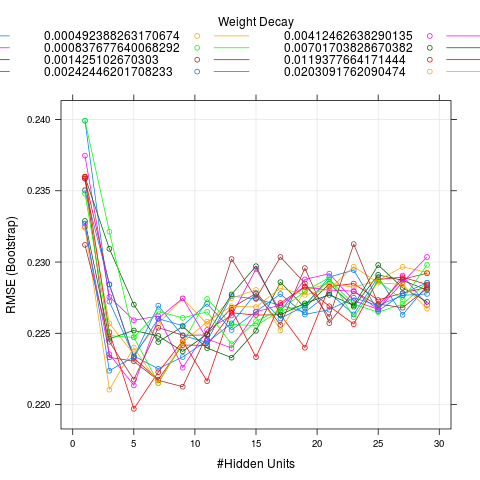
\includegraphics[width=0.6\textwidth]{figs/SI/nnetopt_global.png}
\caption{
  Optimisation for neural network hyperparameters trained on the global dataset.
}

\end{figure}


\begin{figure}[h!]
  \centering
  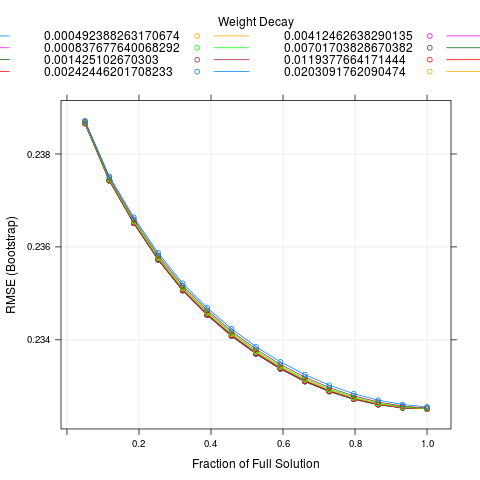
\includegraphics[width=0.6\textwidth]{figs/SI/enetopt_global.png}
\caption{
  Optimisation for elastic net hyperparameters trained on the global dataset.
}
\end{figure}



\begin{figure}[h!]
  \centering
  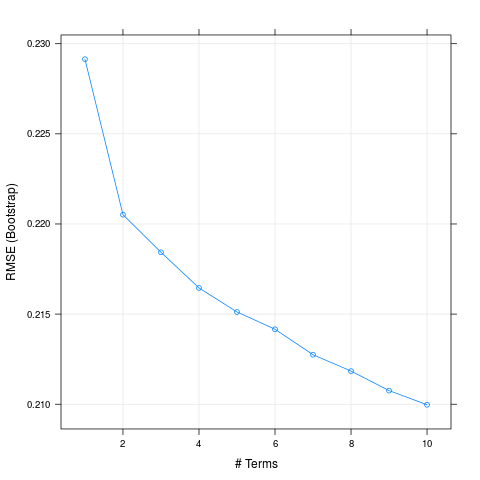
\includegraphics[width=0.6\textwidth]{figs/SI/ppropt.png}
\caption{
  Optimisation for PPR hyperparameters trained on the global dataset.
}

\end{figure}




\clearpage
%%%%%%%%%%%%%%%%%%%%%%%%%%%%%%%%%%%%%%%%%%%%%%%%%%%%%%%%%%%%%%%%%%%%%%%
\section{Colombia (South America) prevalence dataset Machine Learning}
%%%%%%%%%%%%%%%%%%%%%%%%%%%%%%%%%%%%%%%%%%%%%%%%%%%%%%%%%%%%%%%%%%%%%%%


\subsection{Predictions}

\begin{figure}[h!]
  \centering
  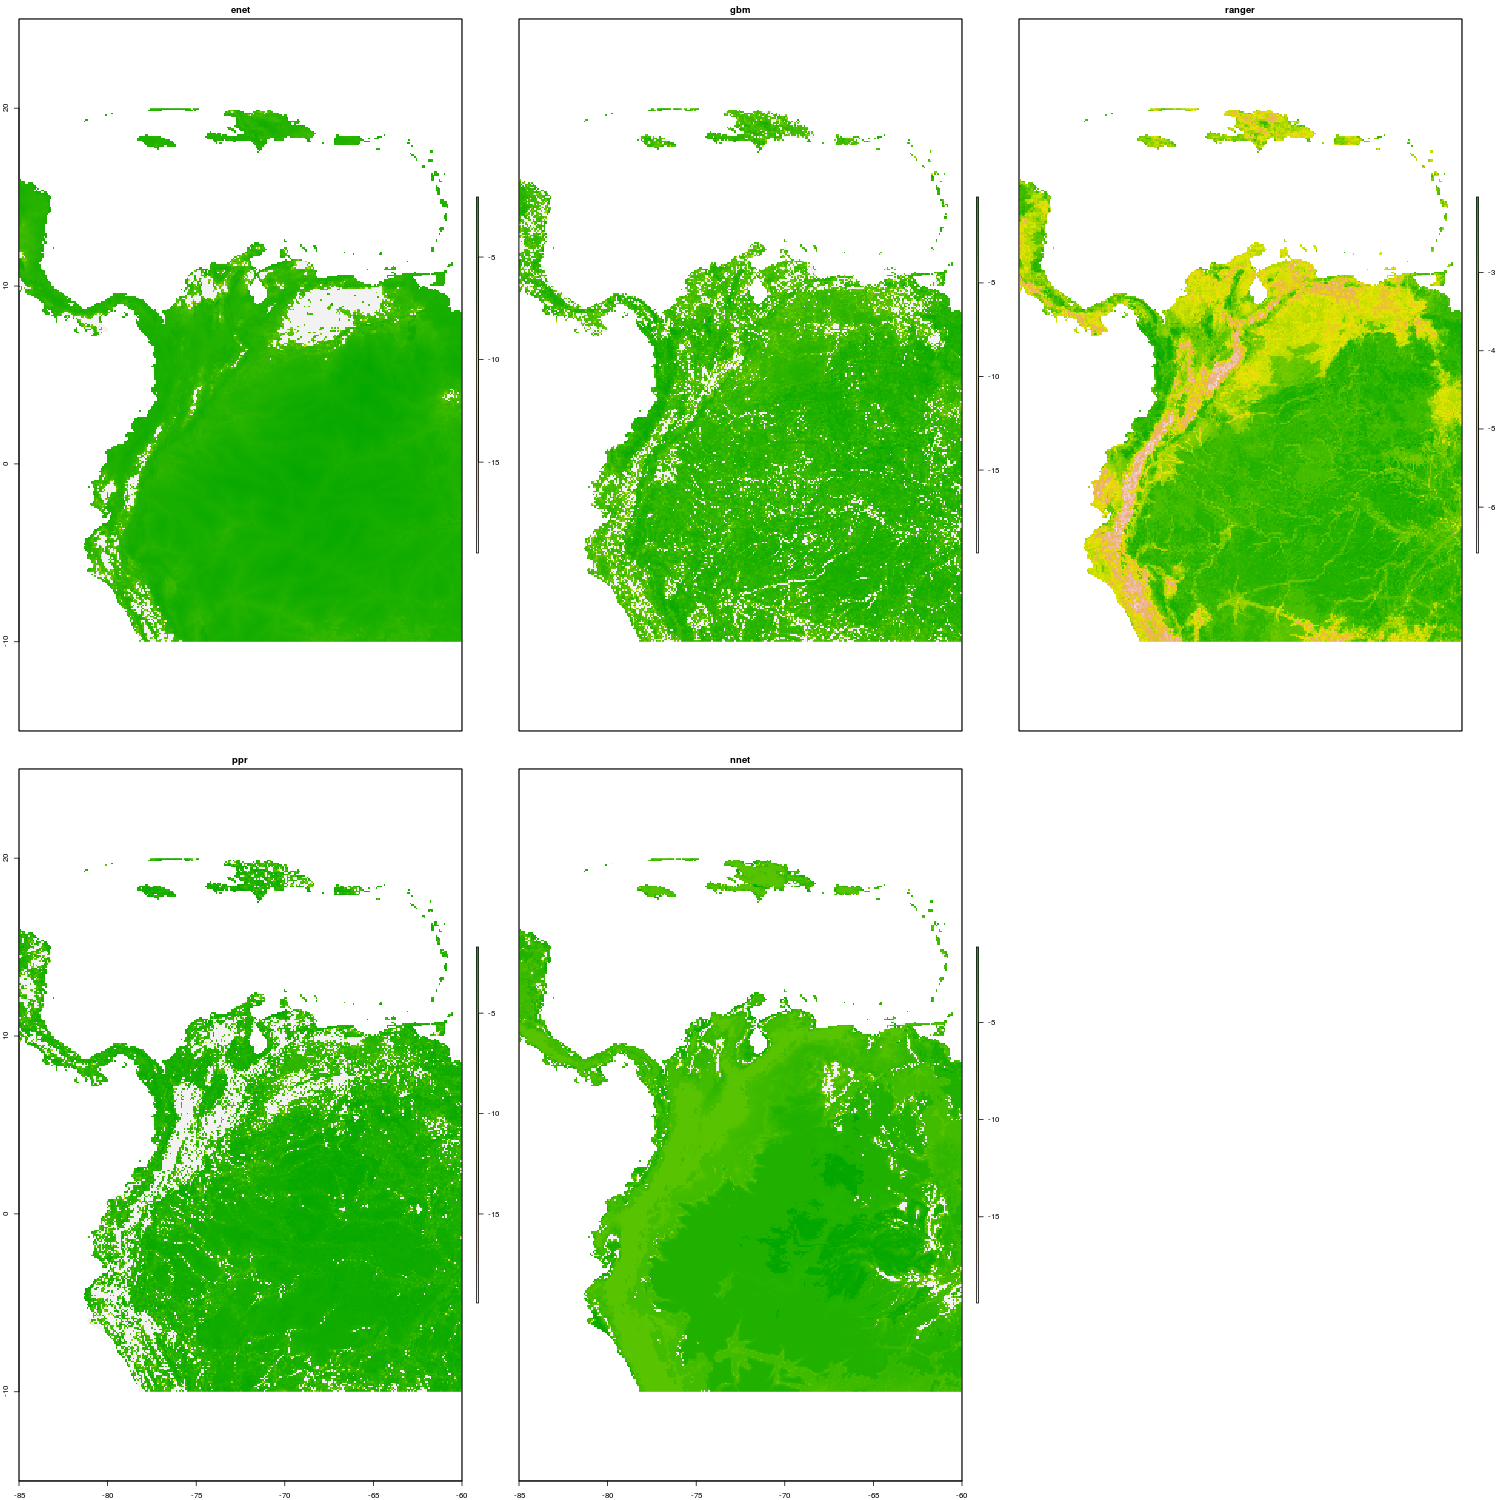
\includegraphics[width=1\textwidth]{figs/SI/SA_all_ml.png}
\caption{
  Predictions from machine learning models trained on South American prevalence data.
}

\end{figure}


\begin{figure}[h!]
  \centering
  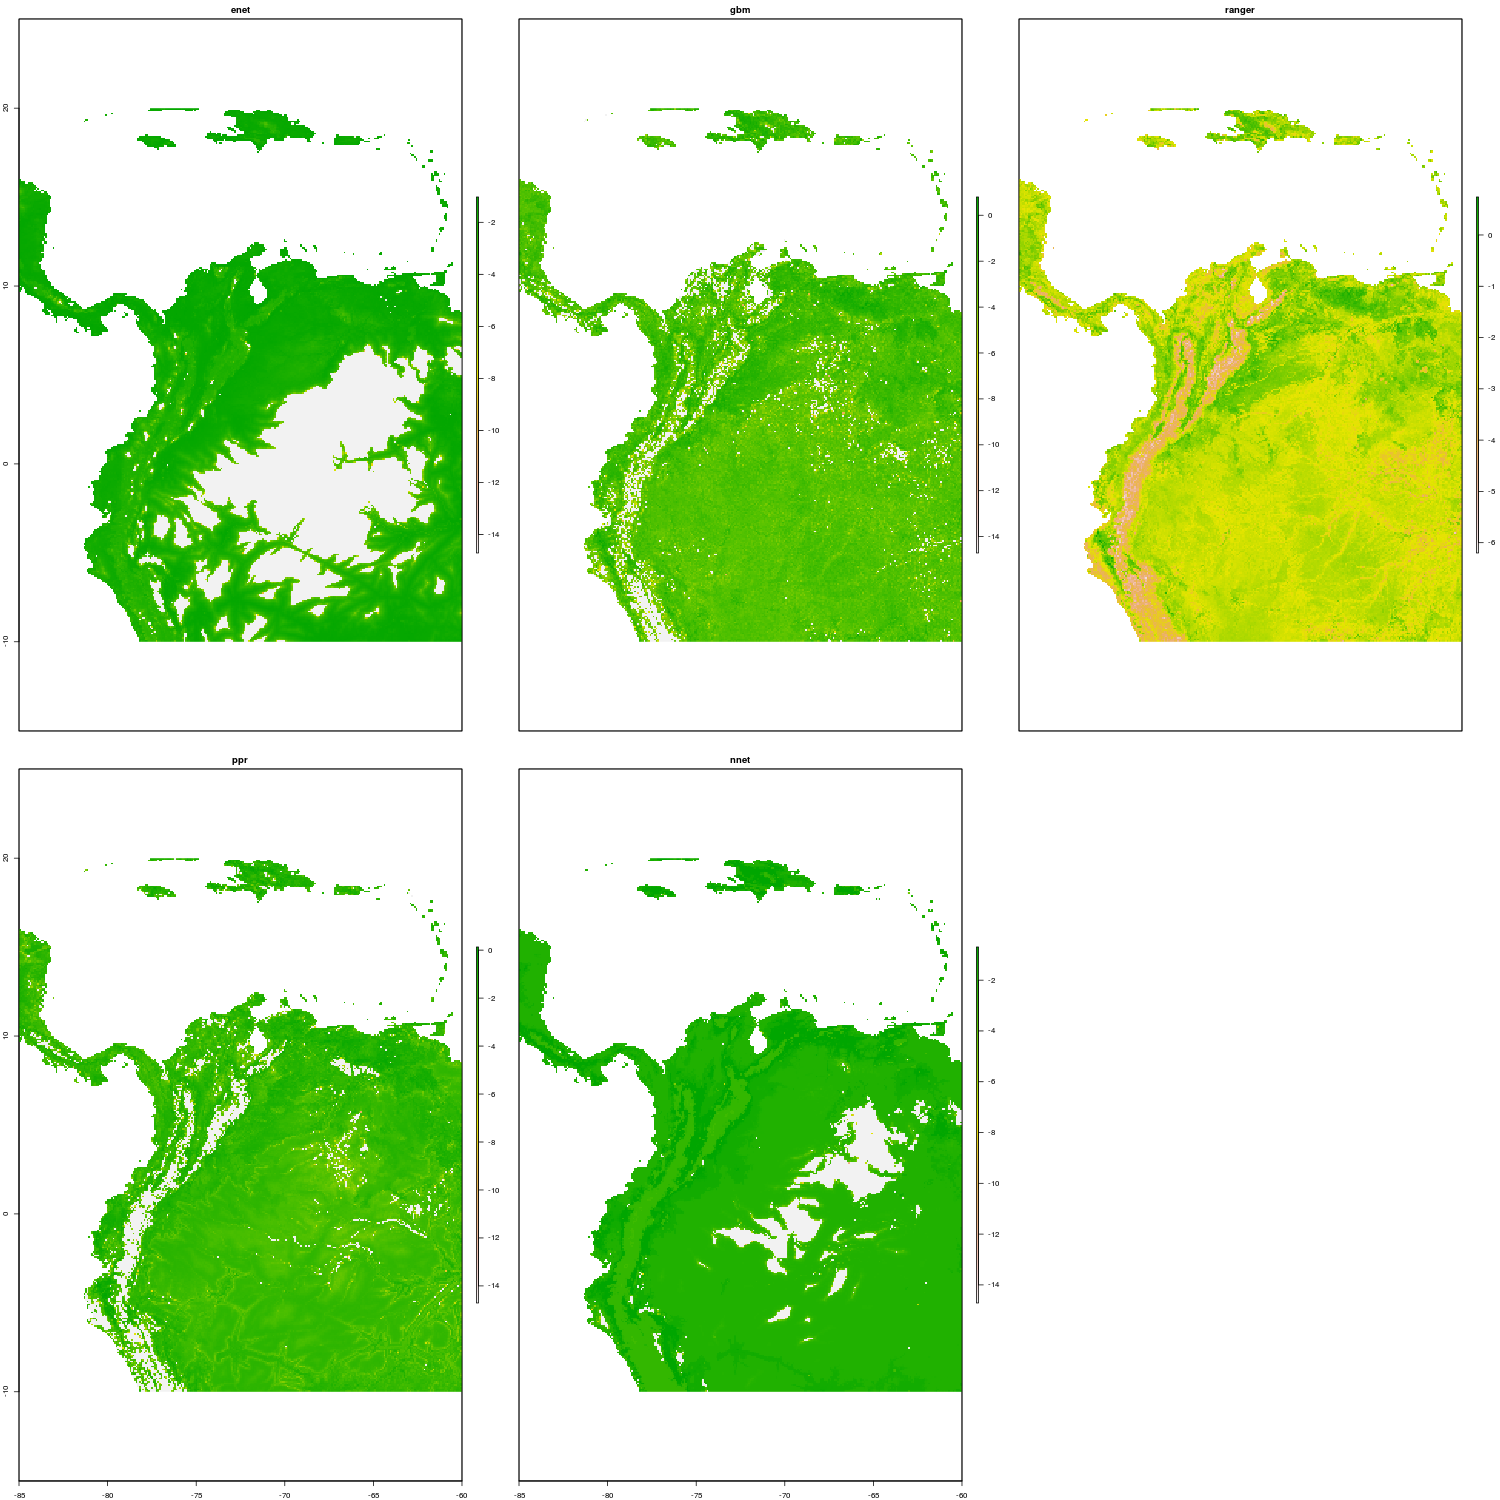
\includegraphics[width=1\textwidth]{figs/SI/COL_all_globalml.png}
\caption{
  Predictions over Colombia from machine learning models trained on global prevalence data.
}

\end{figure}




\clearpage
\subsection{Out-of-sample scatter plots}


\begin{figure}[h!]
  \centering
  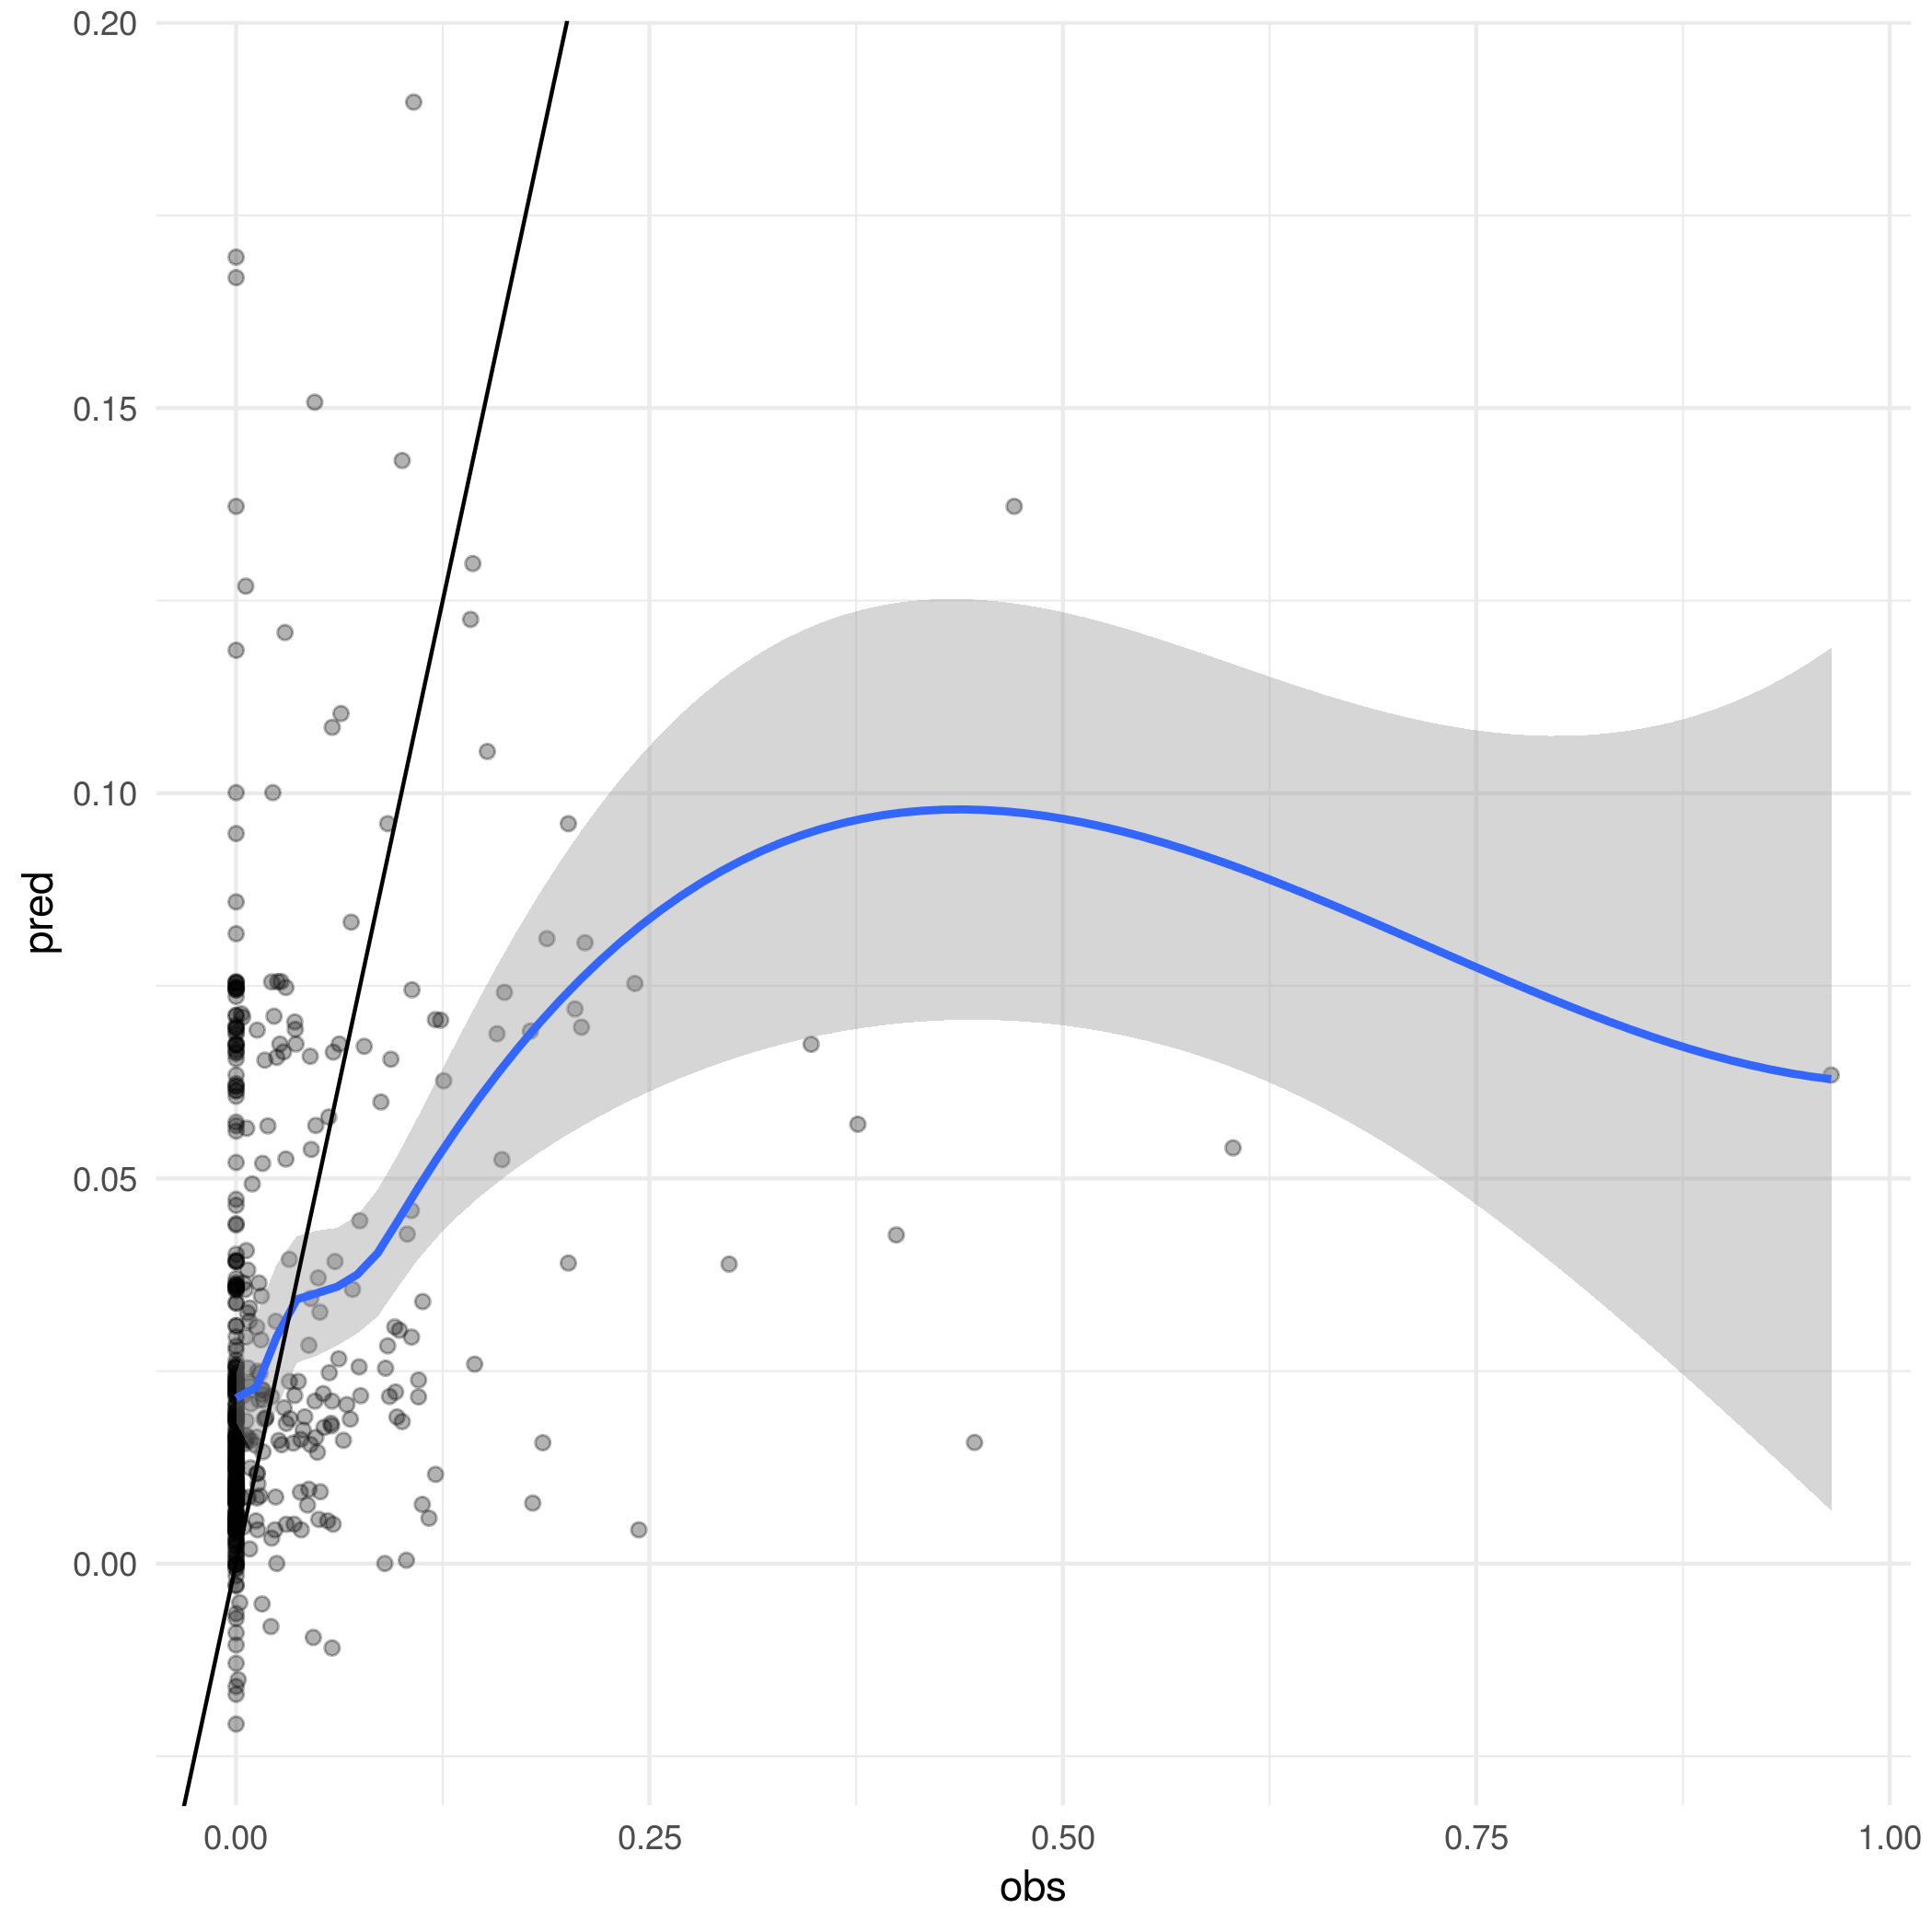
\includegraphics[width=0.6\textwidth]{figs/SI/nnet_obspred_sa.png}
\caption{
  Scatter plot of predictions and held out observed data for the neural network trained on the South America dataset.
}

\end{figure}



\begin{figure}[h!]
  \centering
  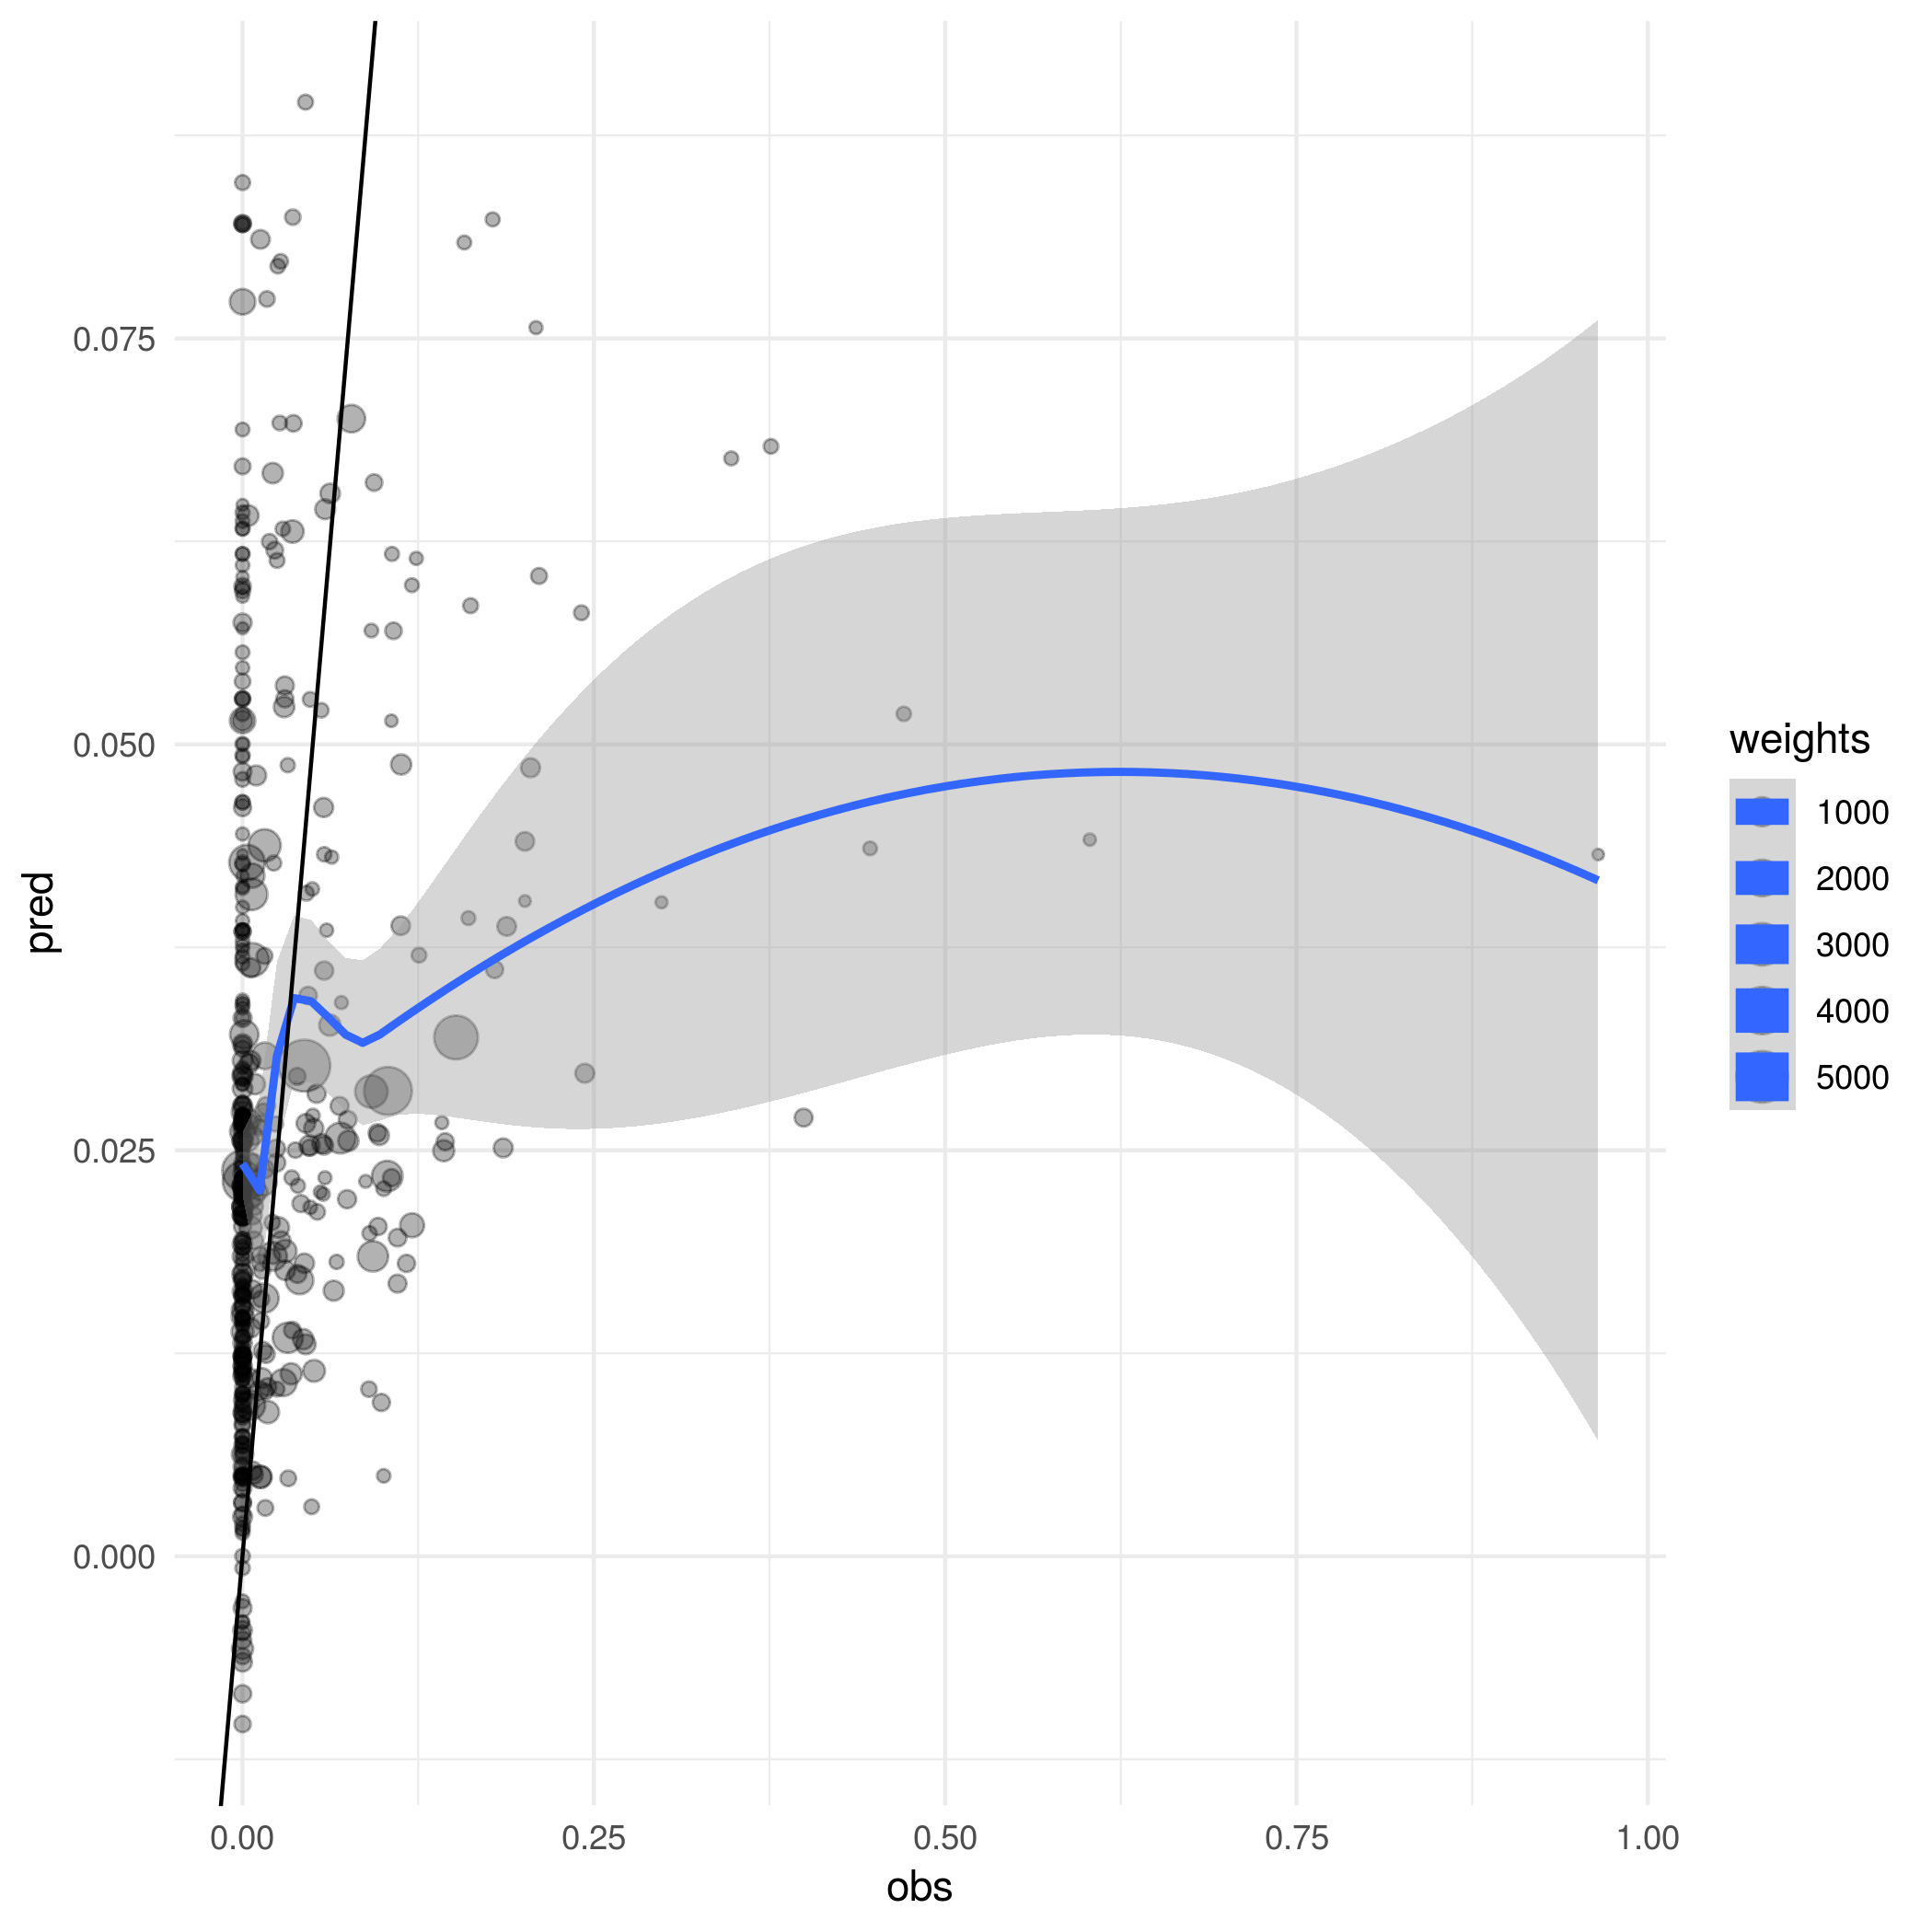
\includegraphics[width=0.6\textwidth]{figs/SI/enet_obspred_sa.png}
\caption{
  Scatter plot of predictions and held out observed data for the elastic net trained on the South America dataset.
}

\end{figure}


\begin{figure}[h!]
  \centering
  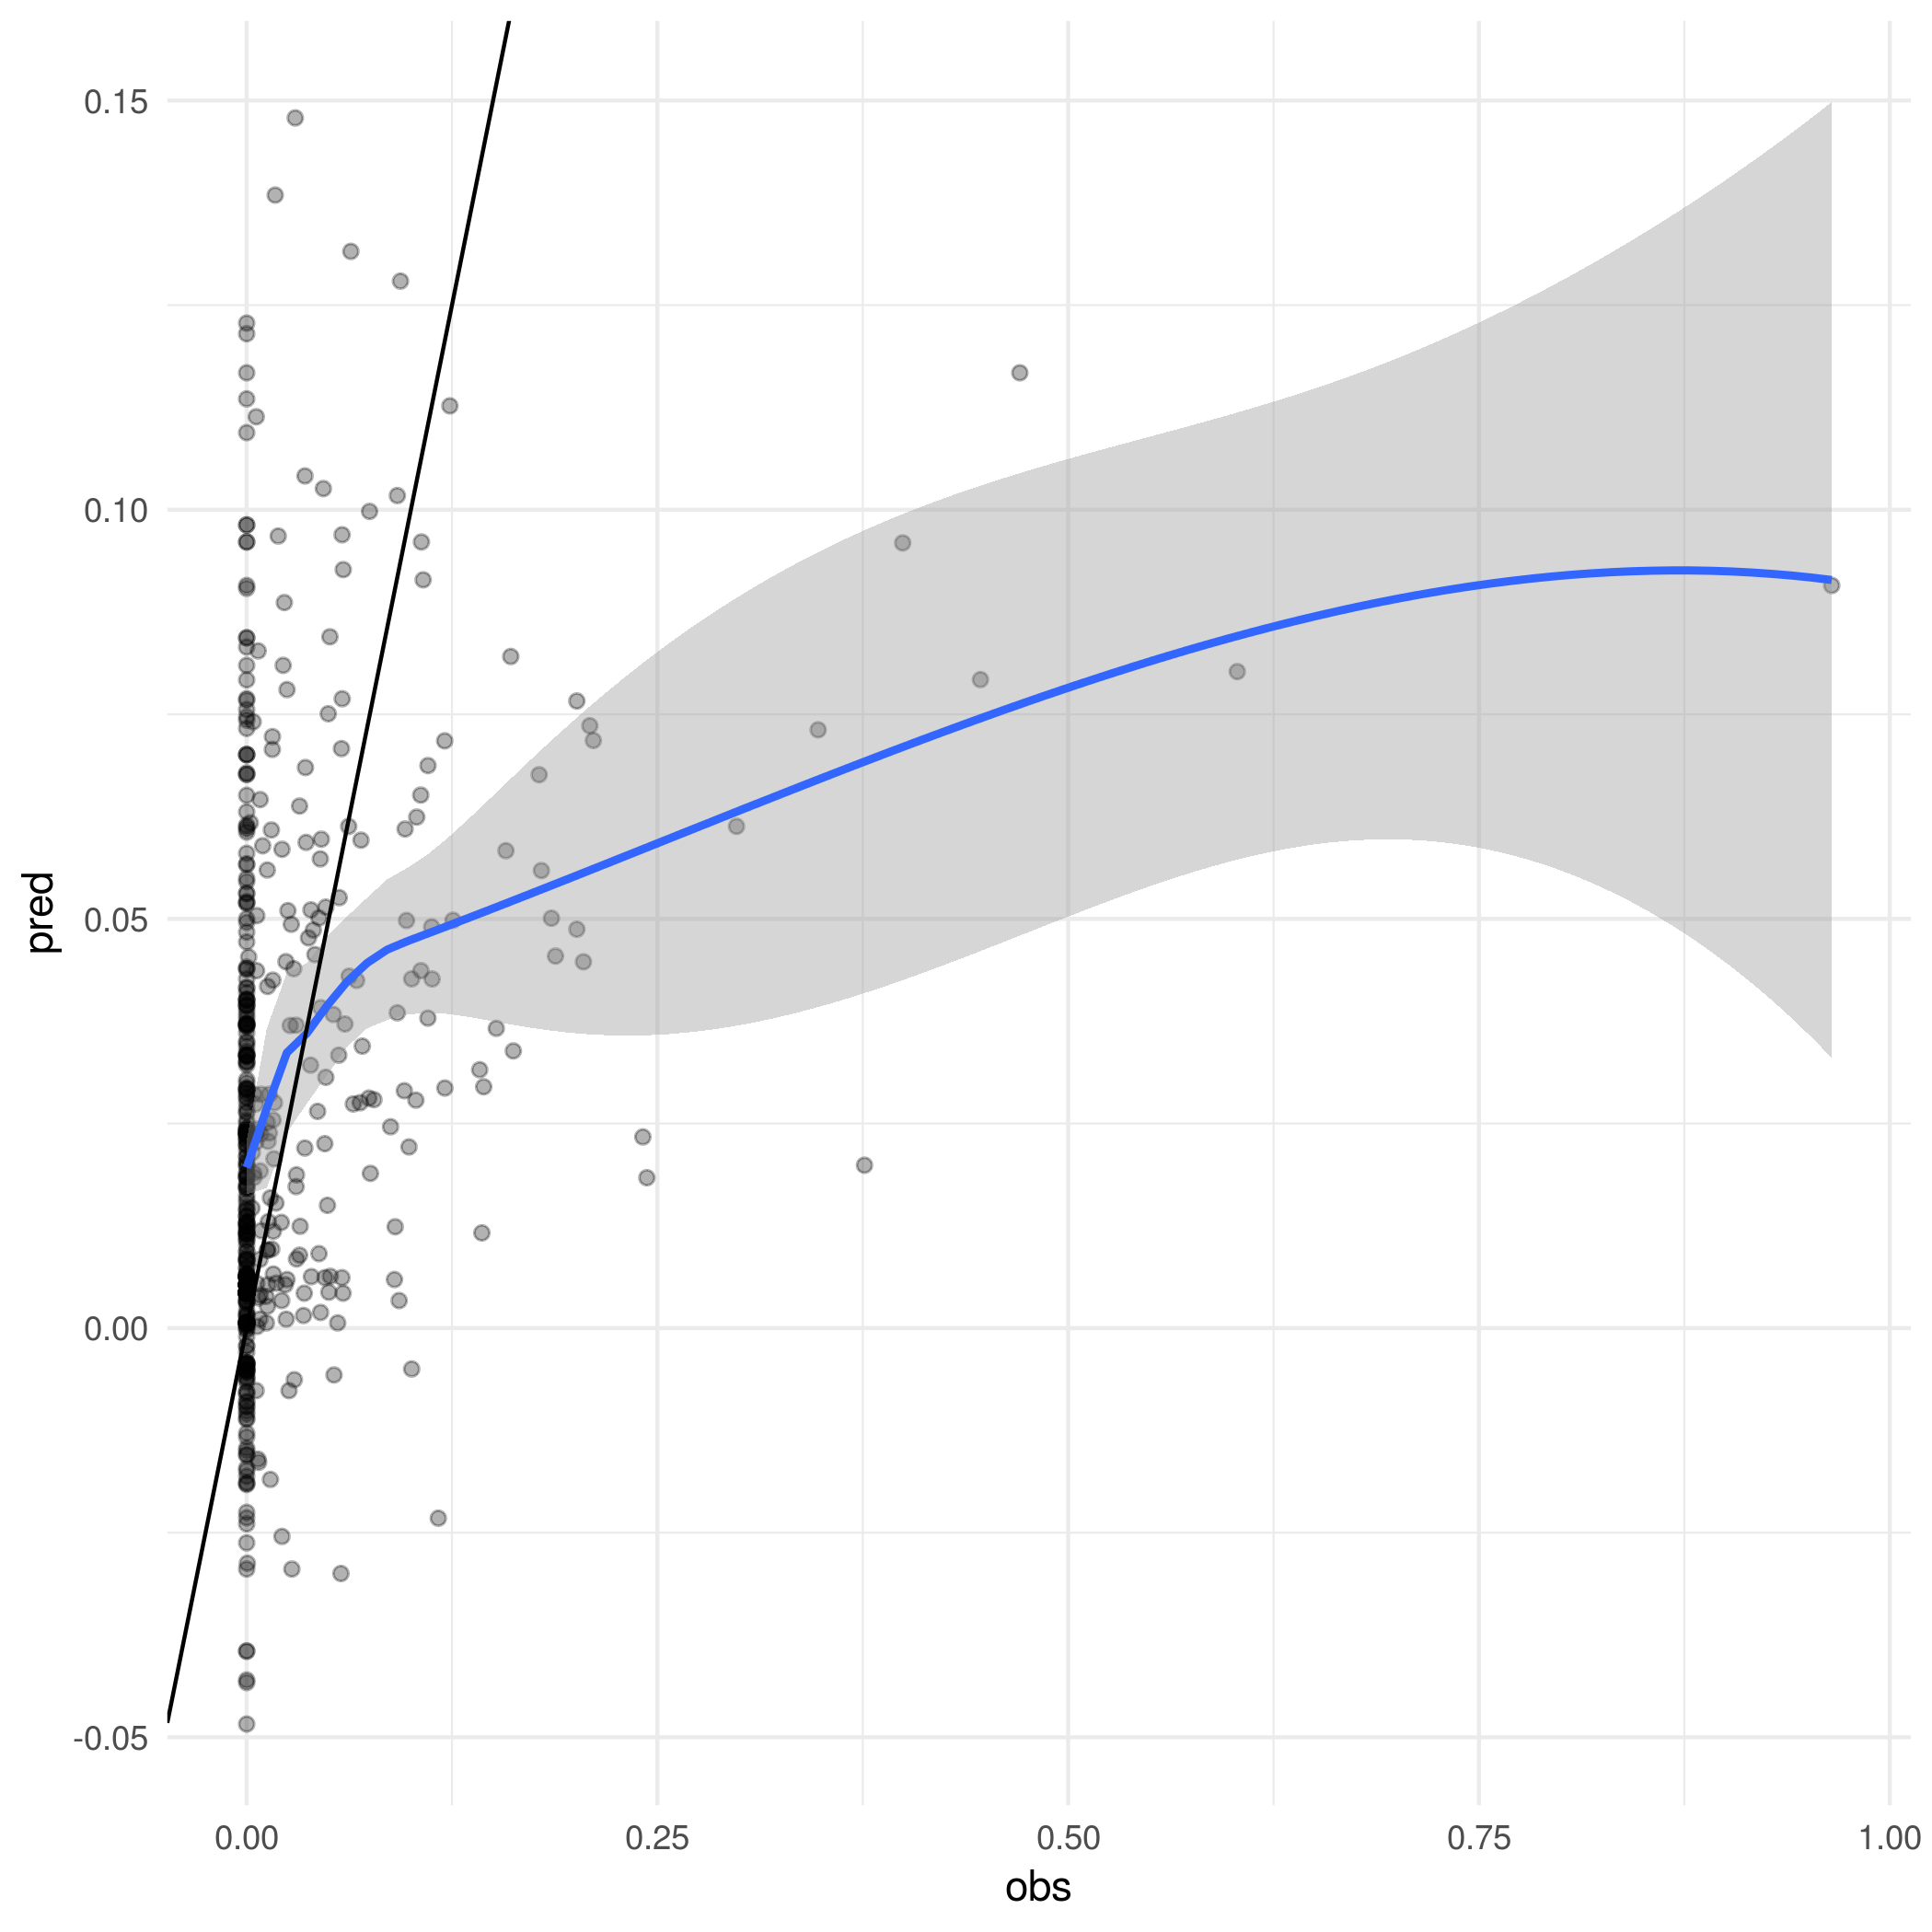
\includegraphics[width=0.6\textwidth]{figs/SI/ppr_obspred_sa.png}
\caption{
  Scatter plot of predictions and held out observed data for the PPR trained on the South America dataset.
}

\end{figure}


\begin{figure}[h!]
  \centering
  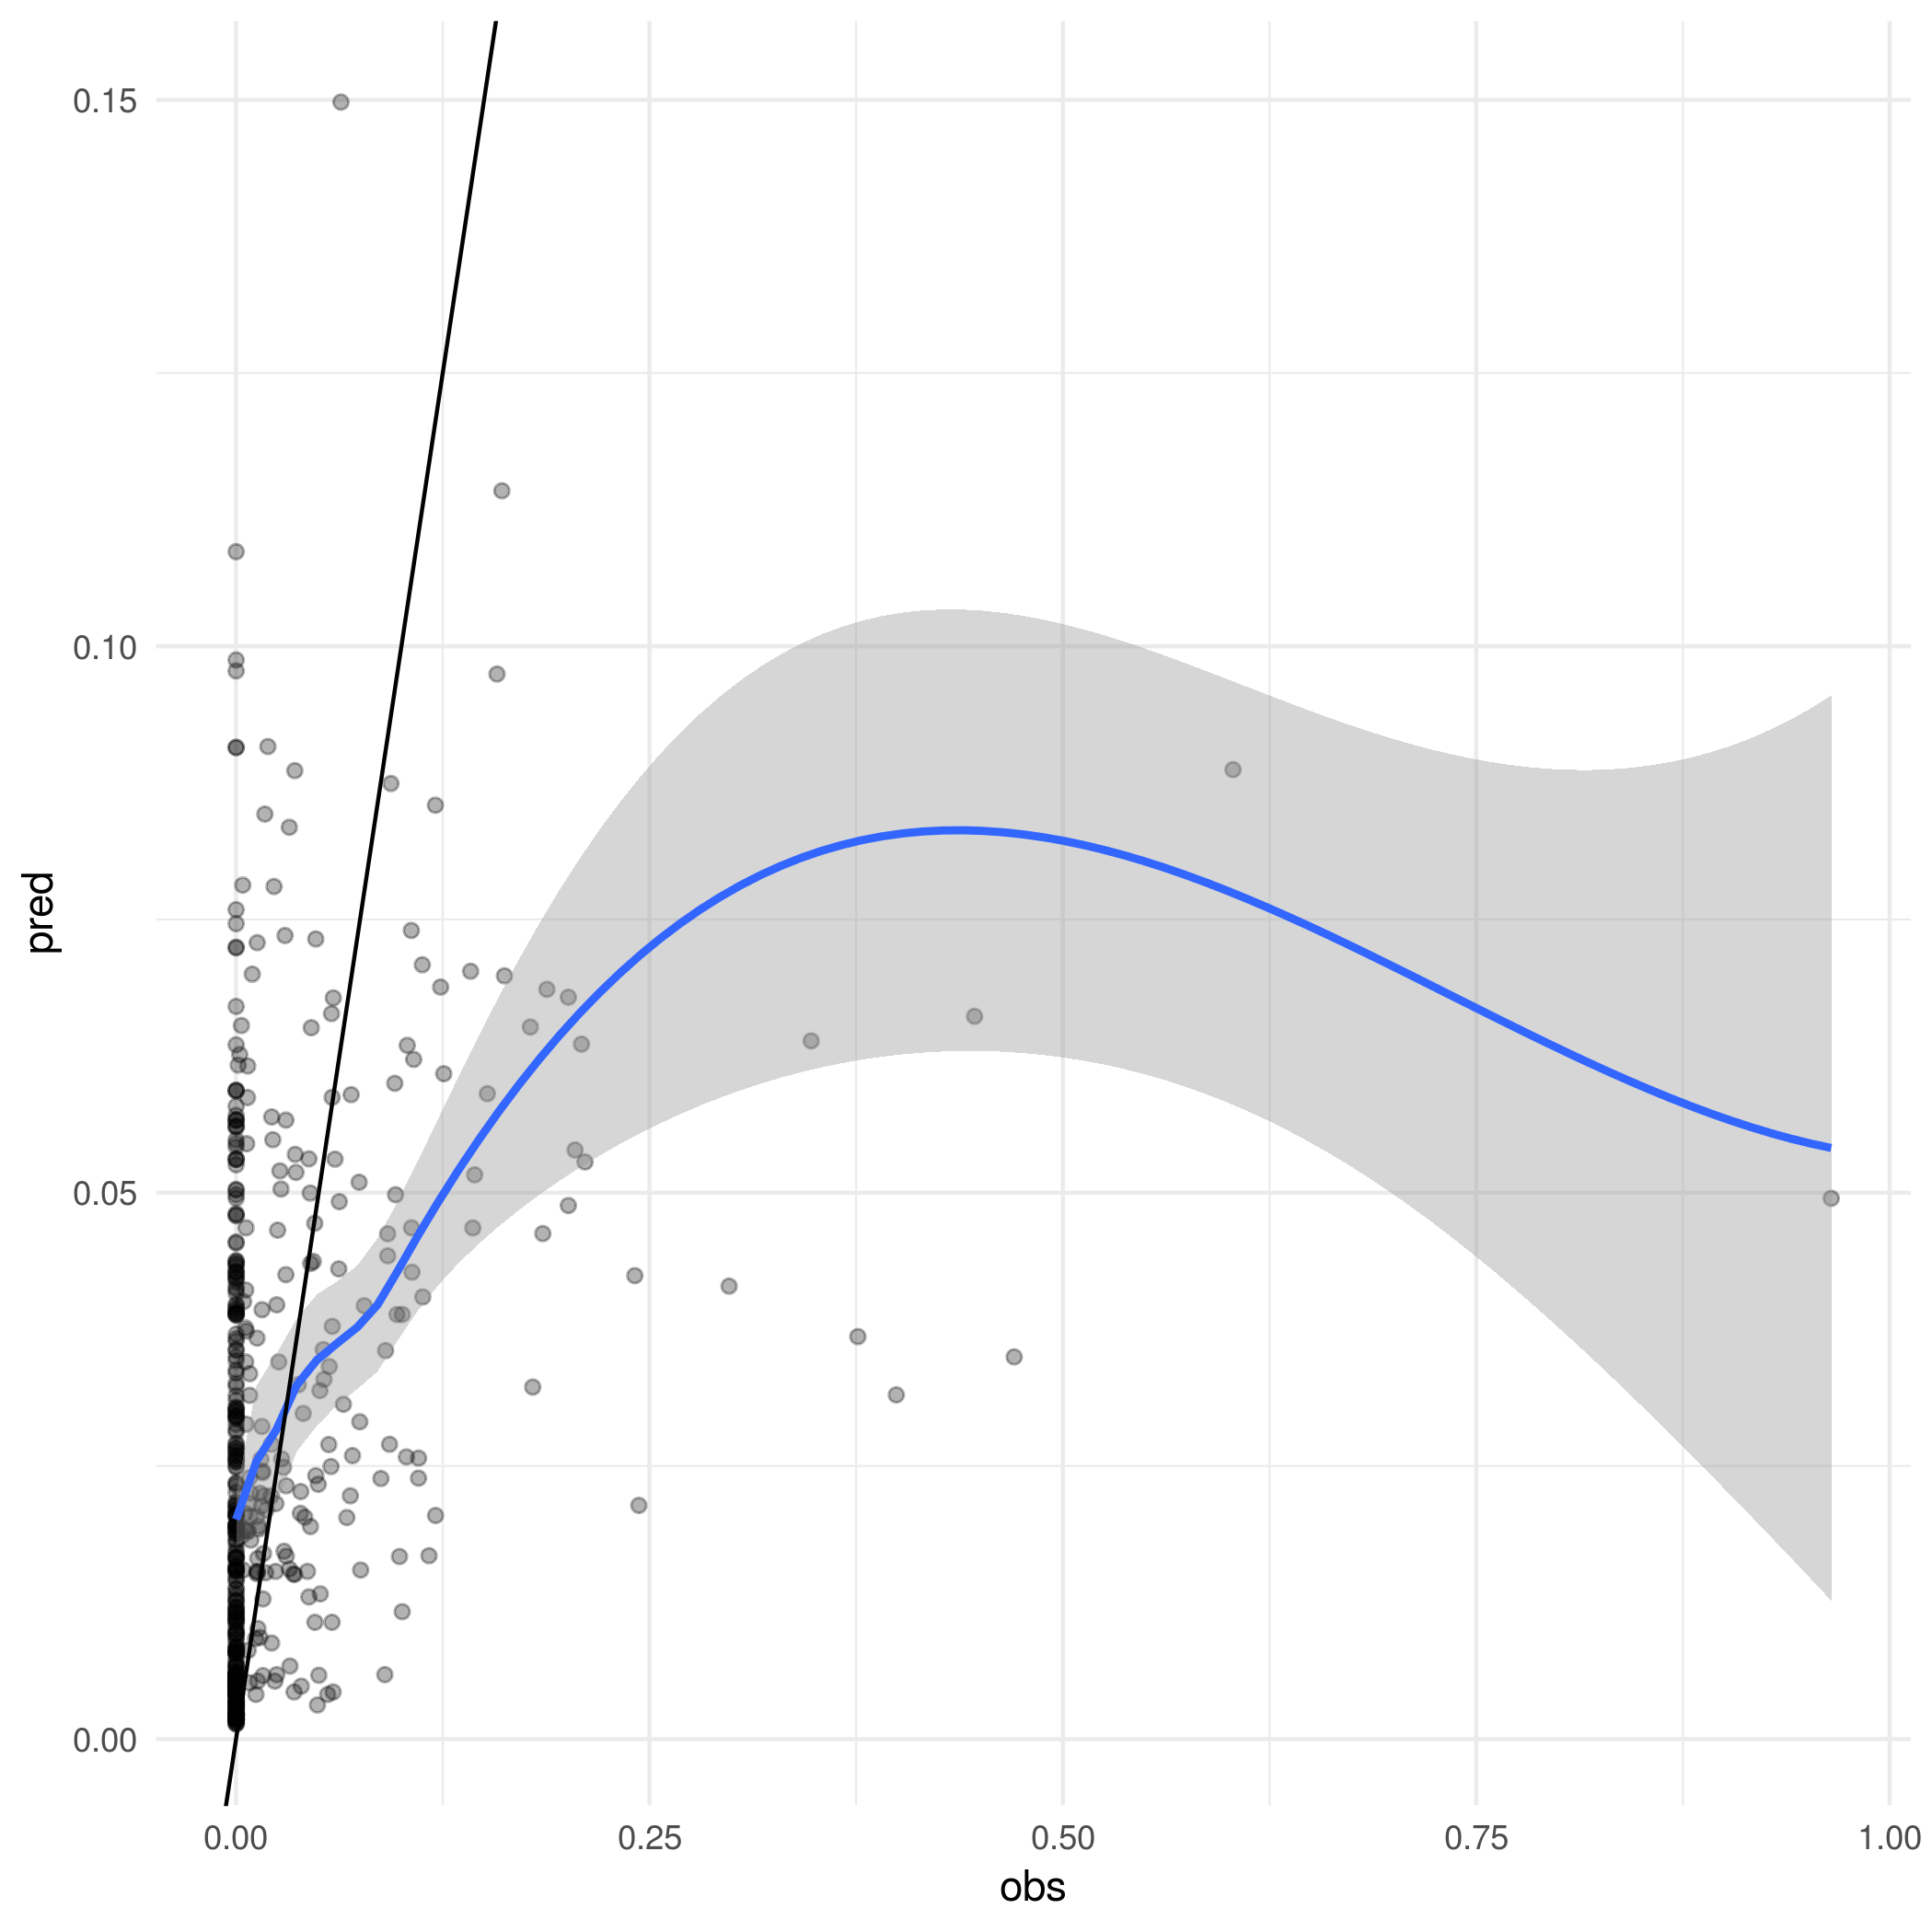
\includegraphics[width=0.6\textwidth]{figs/SI/ranger_obspred_sa.png}
\caption{
  Scatter plot of predictions and held out observed data for the Random Forest trained on the South America dataset.
}

\end{figure}


\begin{figure}[h!]
  \centering
  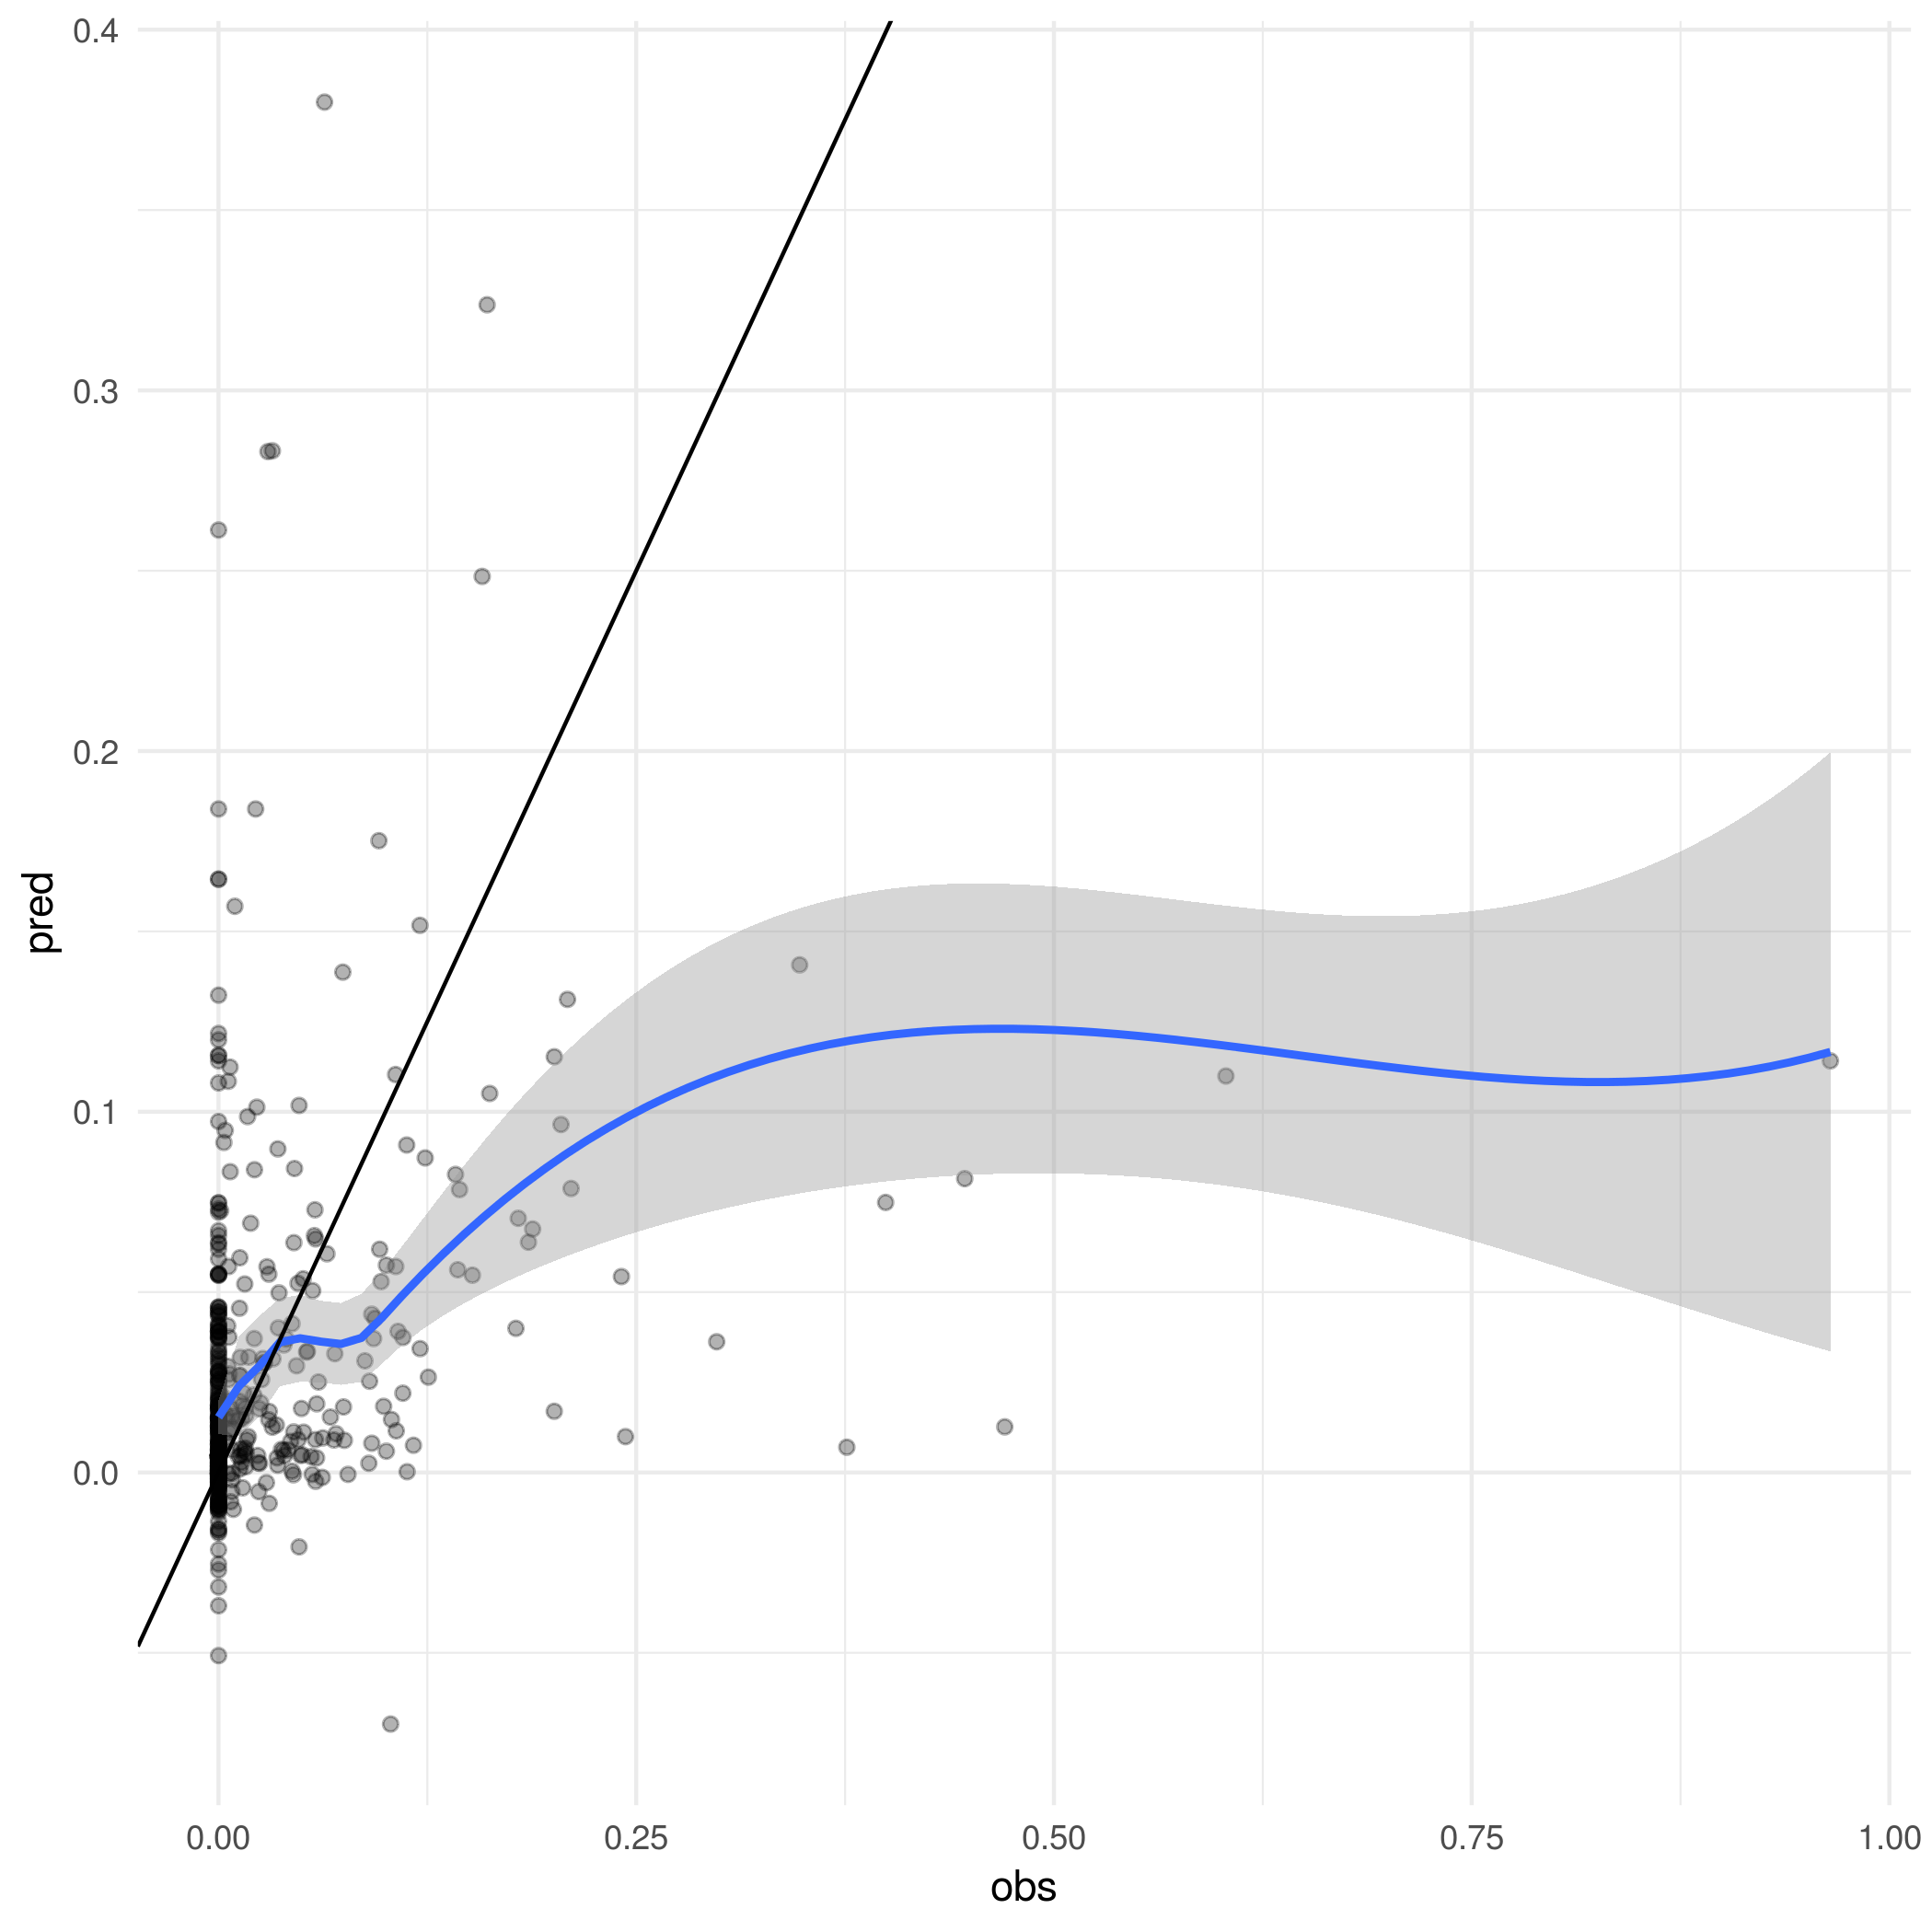
\includegraphics[width=0.6\textwidth]{figs/SI/gbm_obspred_sa.png}
\caption{
  Scatter plot of predictions and held out observed data for the GBM trained on the South America dataset.
}

\end{figure}


\clearpage
\subsection{Hyperparameter optimisation}

As ranger and GBM were tuned with random hyperparameter search, the plots become difficult and are not included.

\begin{figure}[h!]
  \centering
  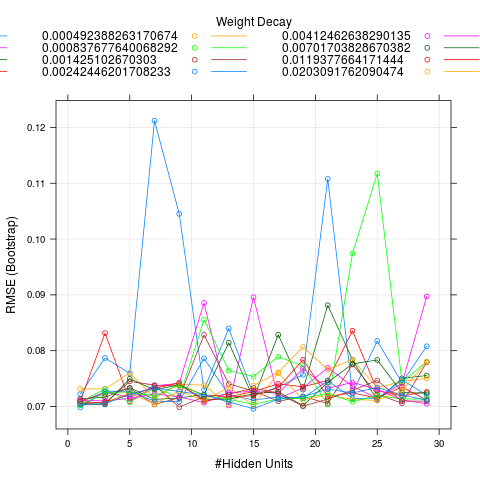
\includegraphics[width=0.6\textwidth]{figs/SI/nnetopt_sa.png}
\caption{
  Optimisation for neural network hyperparameters trained on the South America dataset.
}

\end{figure}


\begin{figure}[h!]
  \centering
  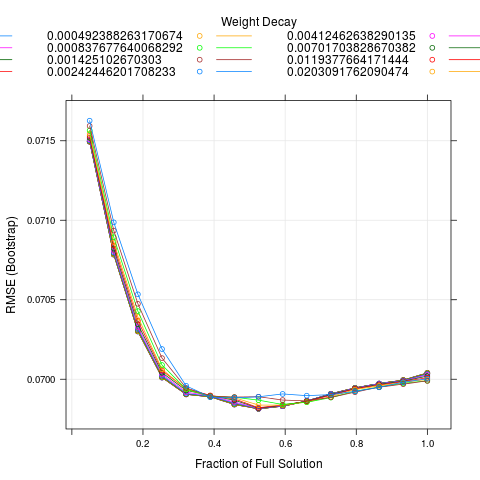
\includegraphics[width=0.6\textwidth]{figs/SI/enetopt_sa.png}
\caption{
  Optimisation for elastic net hyperparameters trained on the South America dataset.
}
\end{figure}



\begin{figure}[h!]
  \centering
  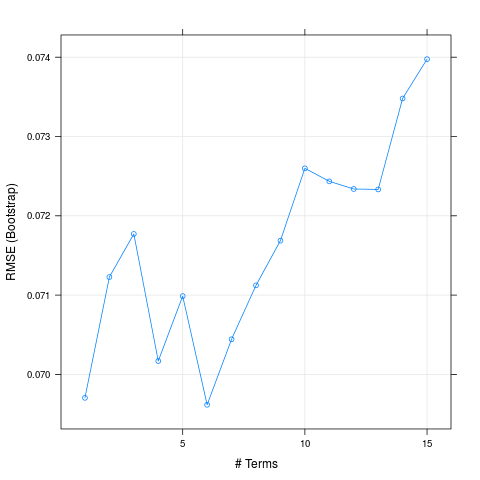
\includegraphics[width=0.6\textwidth]{figs/SI/ppropt_sa.png}
\caption{
  Optimisation for PPR hyperparameters trained on the South America dataset.
}

\end{figure}












\clearpage
%%%%%%%%%%%%%%%%%%%%%%%%%%%%%%%%%%%%%%%%%%%%%%%%%%%%%%%%%%%%%%%%%%%%%%%
\section{Indonesia dataset Machine Learning}
%%%%%%%%%%%%%%%%%%%%%%%%%%%%%%%%%%%%%%%%%%%%%%%%%%%%%%%%%%%%%%%%%%%%%%%



\subsection{Predictions}

\begin{figure}[h!]
  \centering
  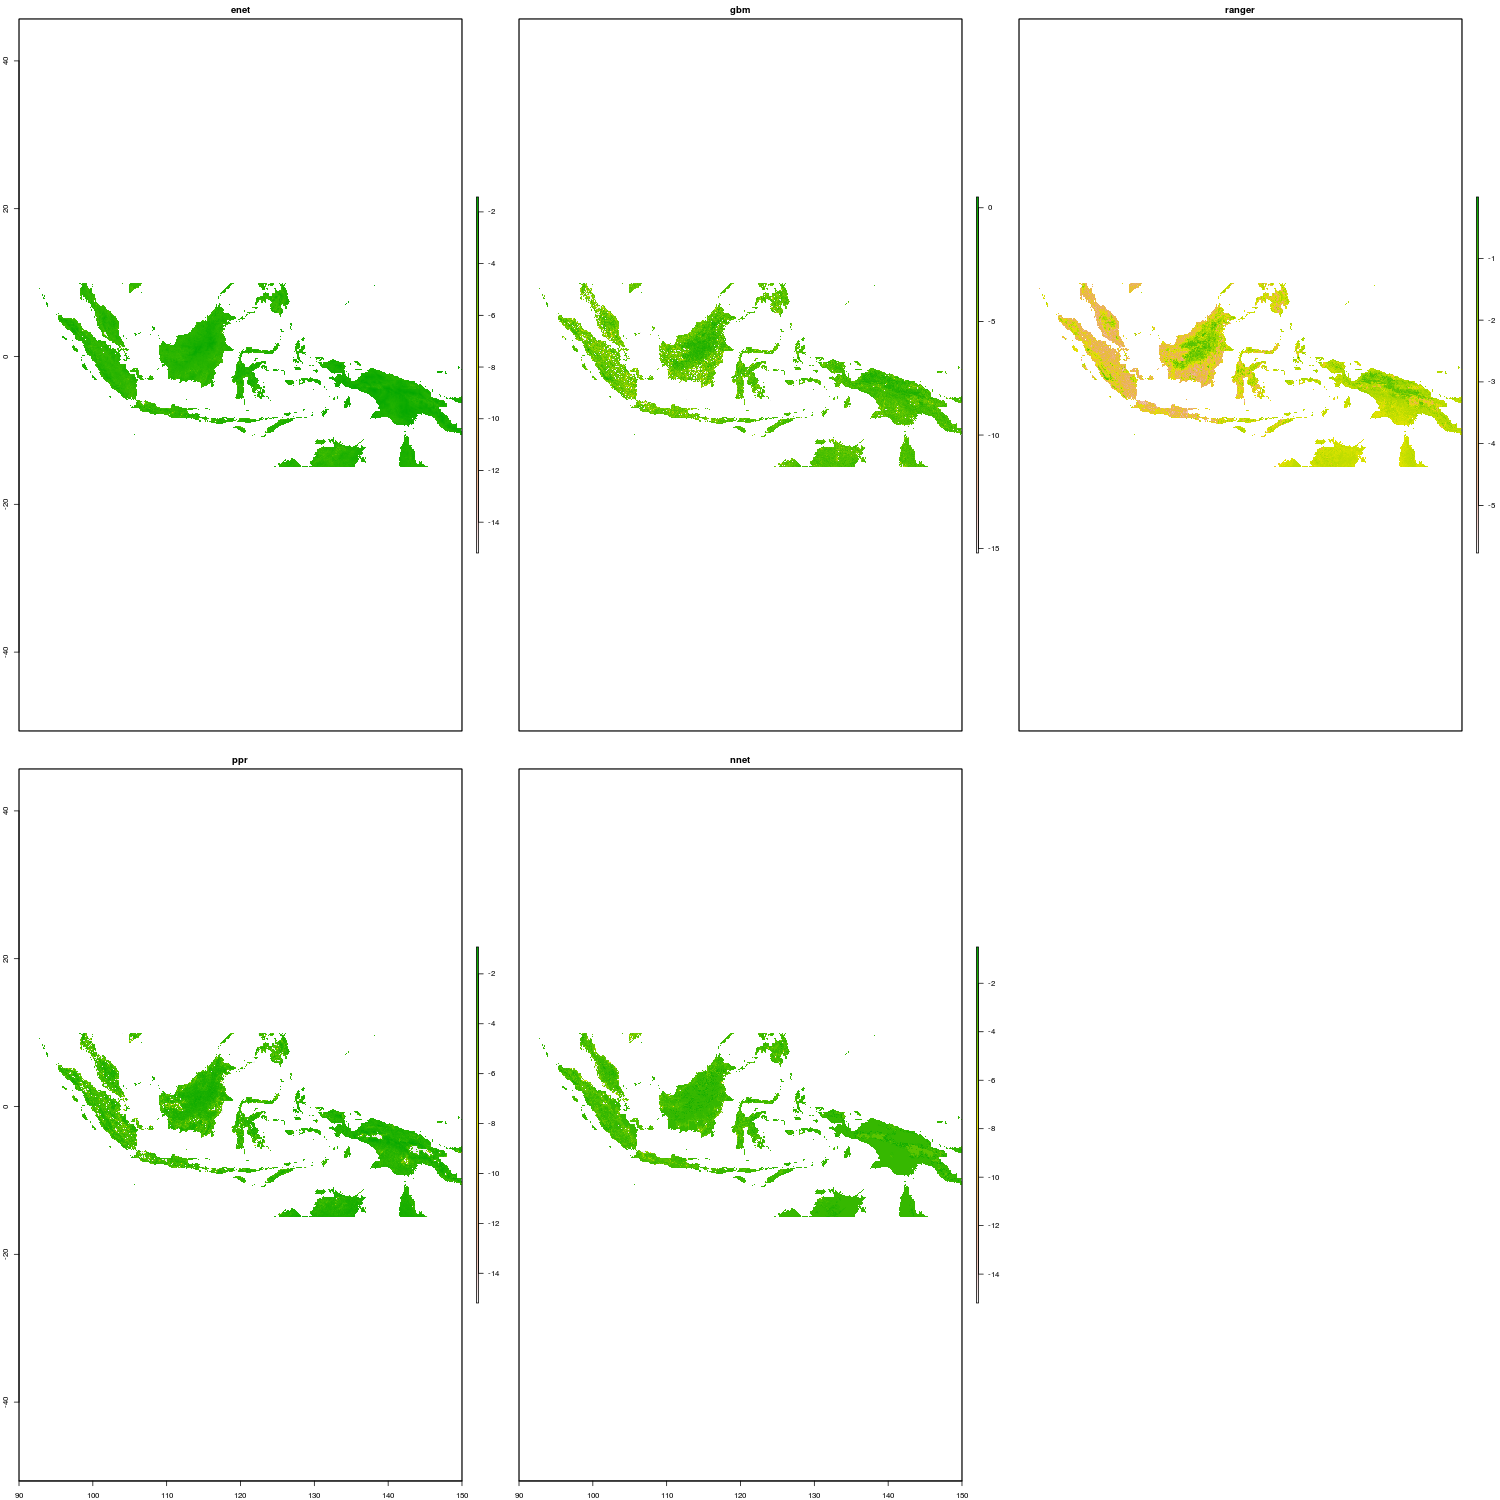
\includegraphics[width=1\textwidth]{figs/SI/idn_all_ml.png}
\caption{
  Predictions from machine learning models trained on Indonesian prevalence data.
}

\end{figure}


\begin{figure}[h!]
  \centering
  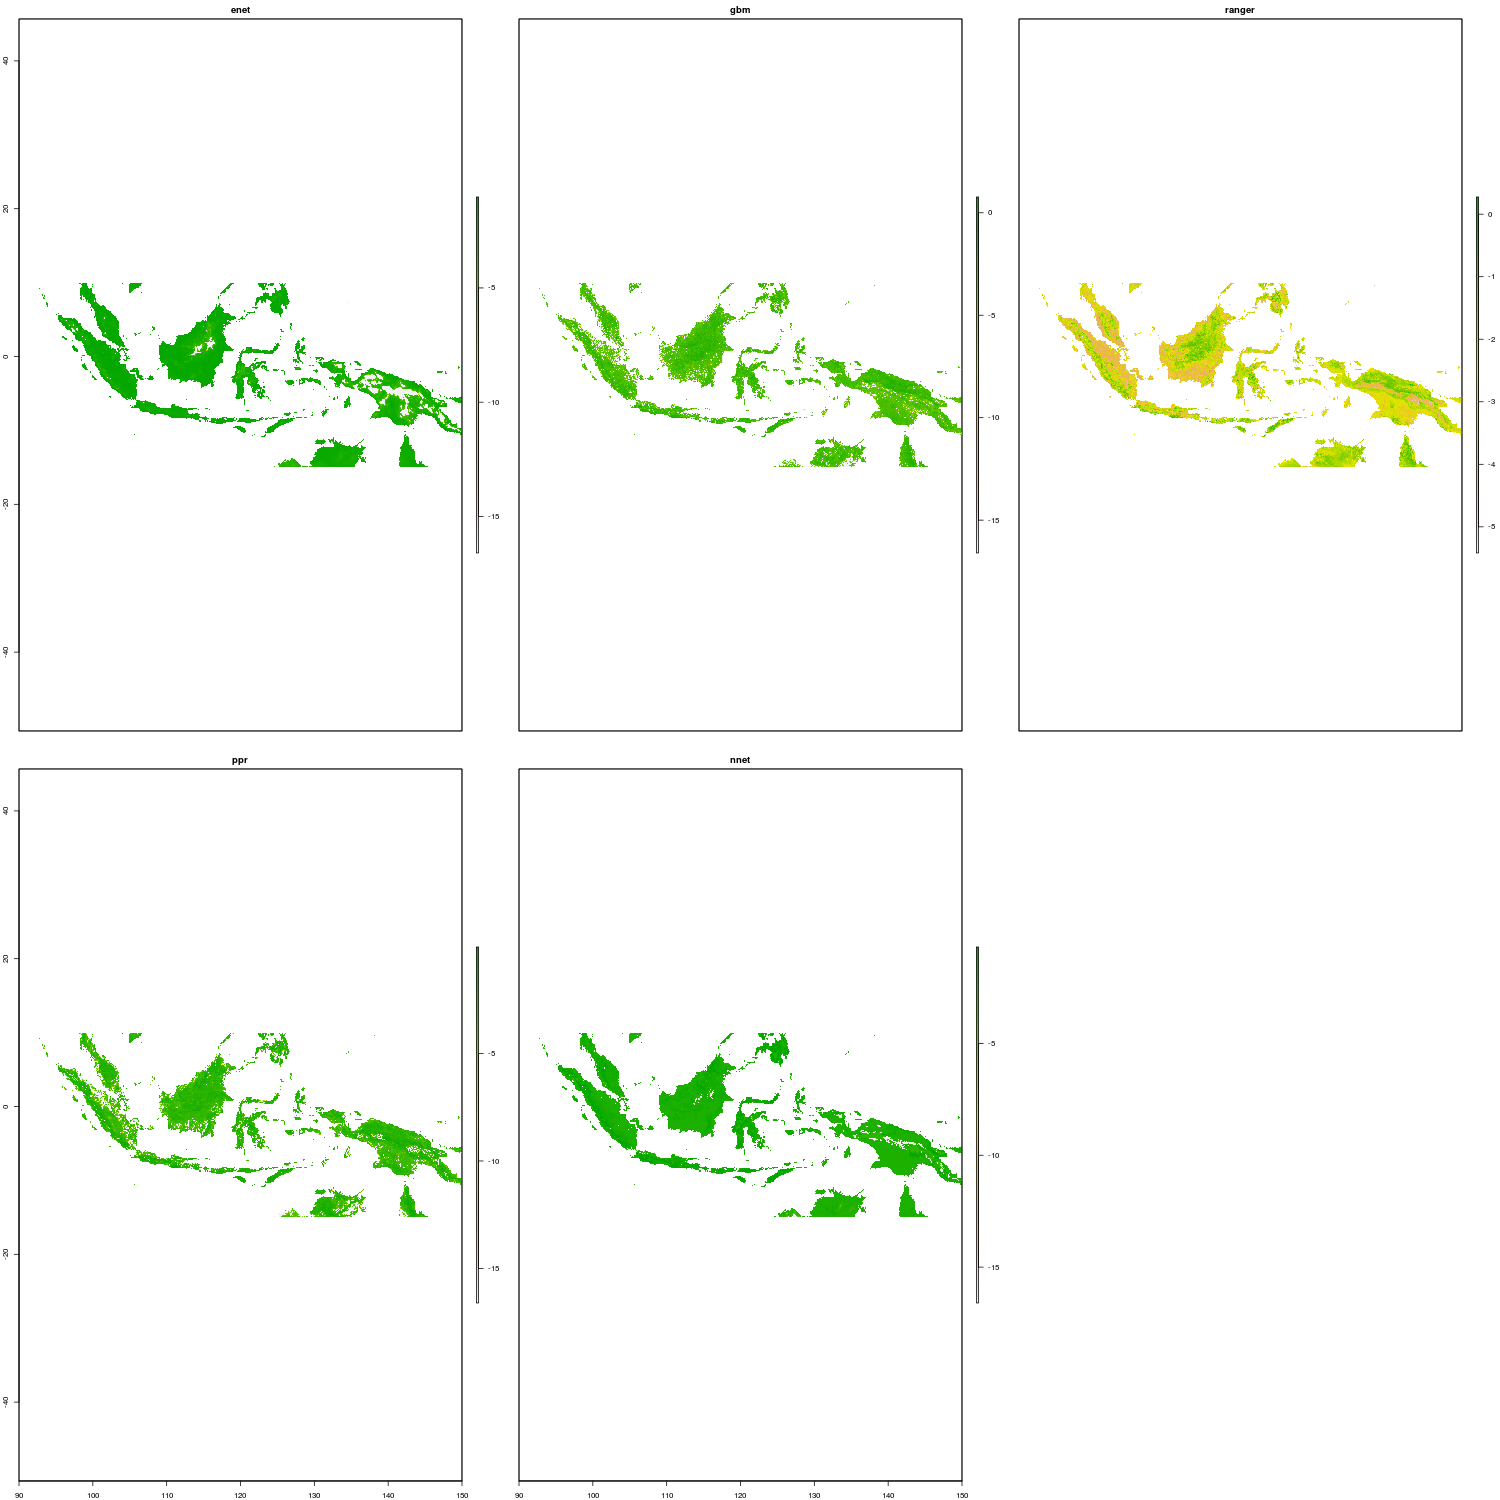
\includegraphics[width=1\textwidth]{figs/SI/idn_all_globalml.png}
\caption{
  Predictions over Indonesia from machine learning models trained on global prevalence data.
}

\end{figure}




\clearpage
\subsection{Out-of-sample scatter plots}


\begin{figure}[h!]
  \centering
  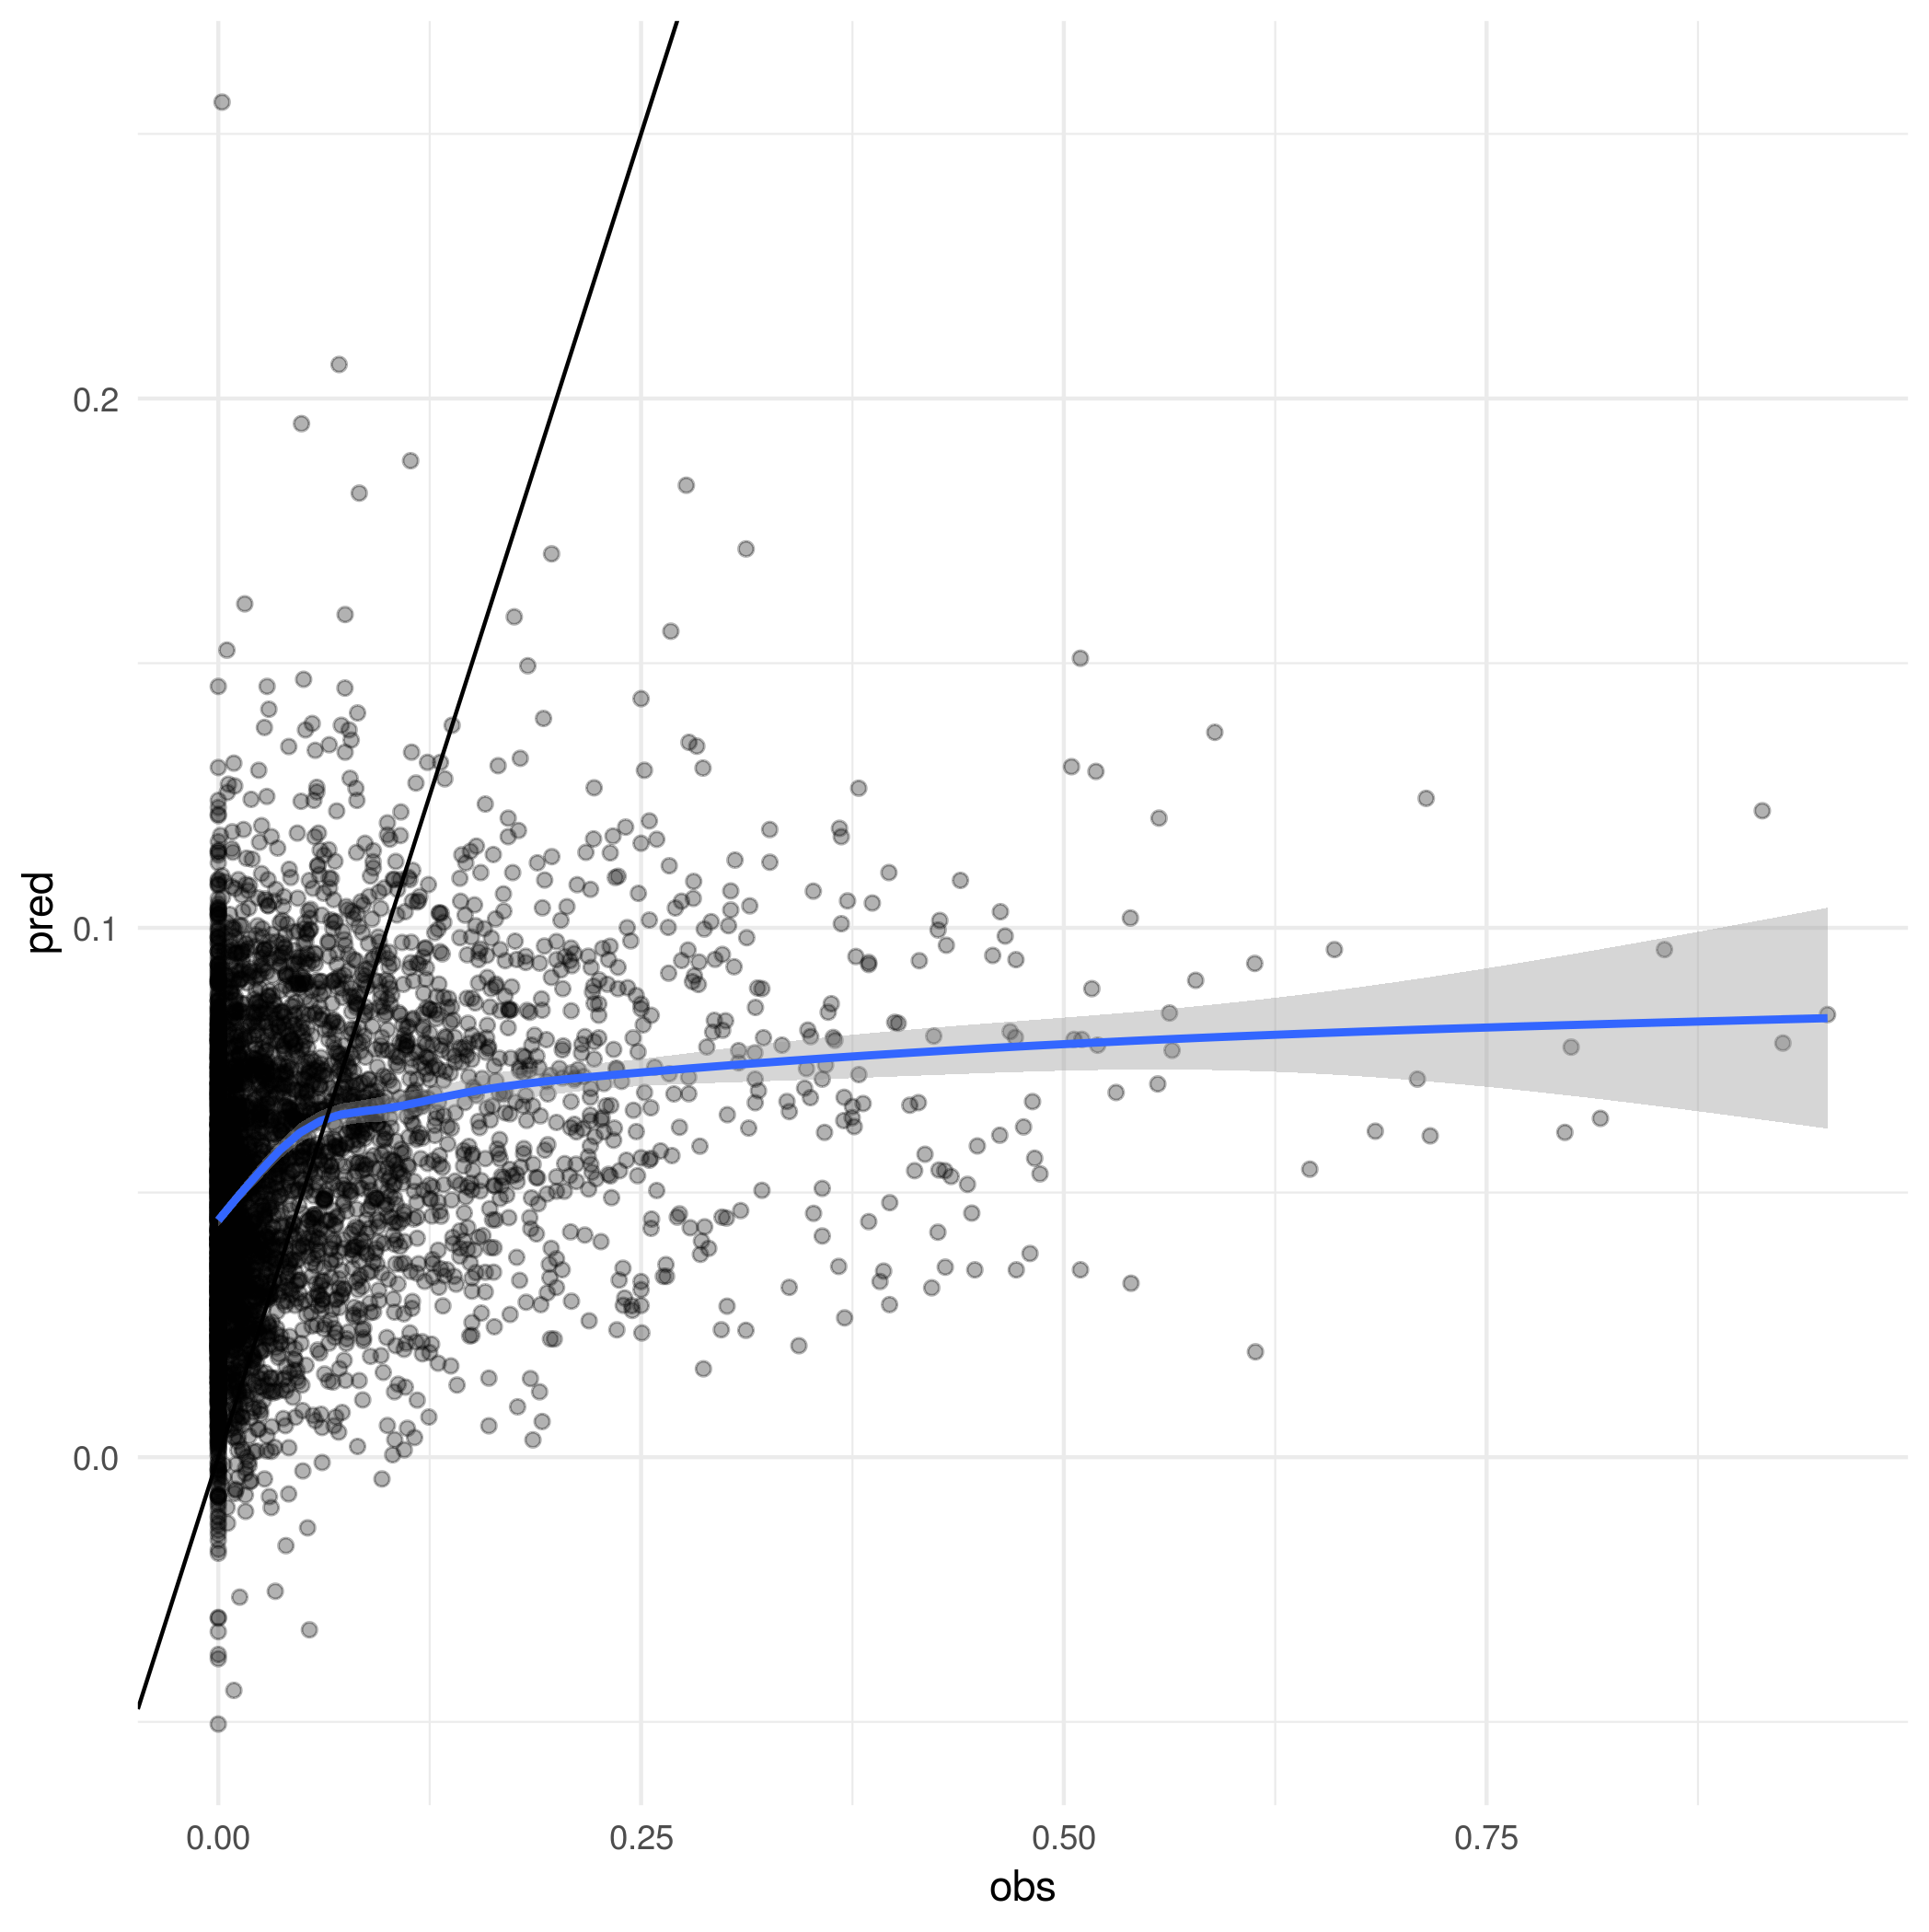
\includegraphics[width=0.6\textwidth]{figs/SI/nnet_obspred_idn.png}
\caption{
  Scatter plot of predictions and held out observed data for the neural network trained on the Indonesia dataset.
}

\end{figure}



\begin{figure}[h!]
  \centering
  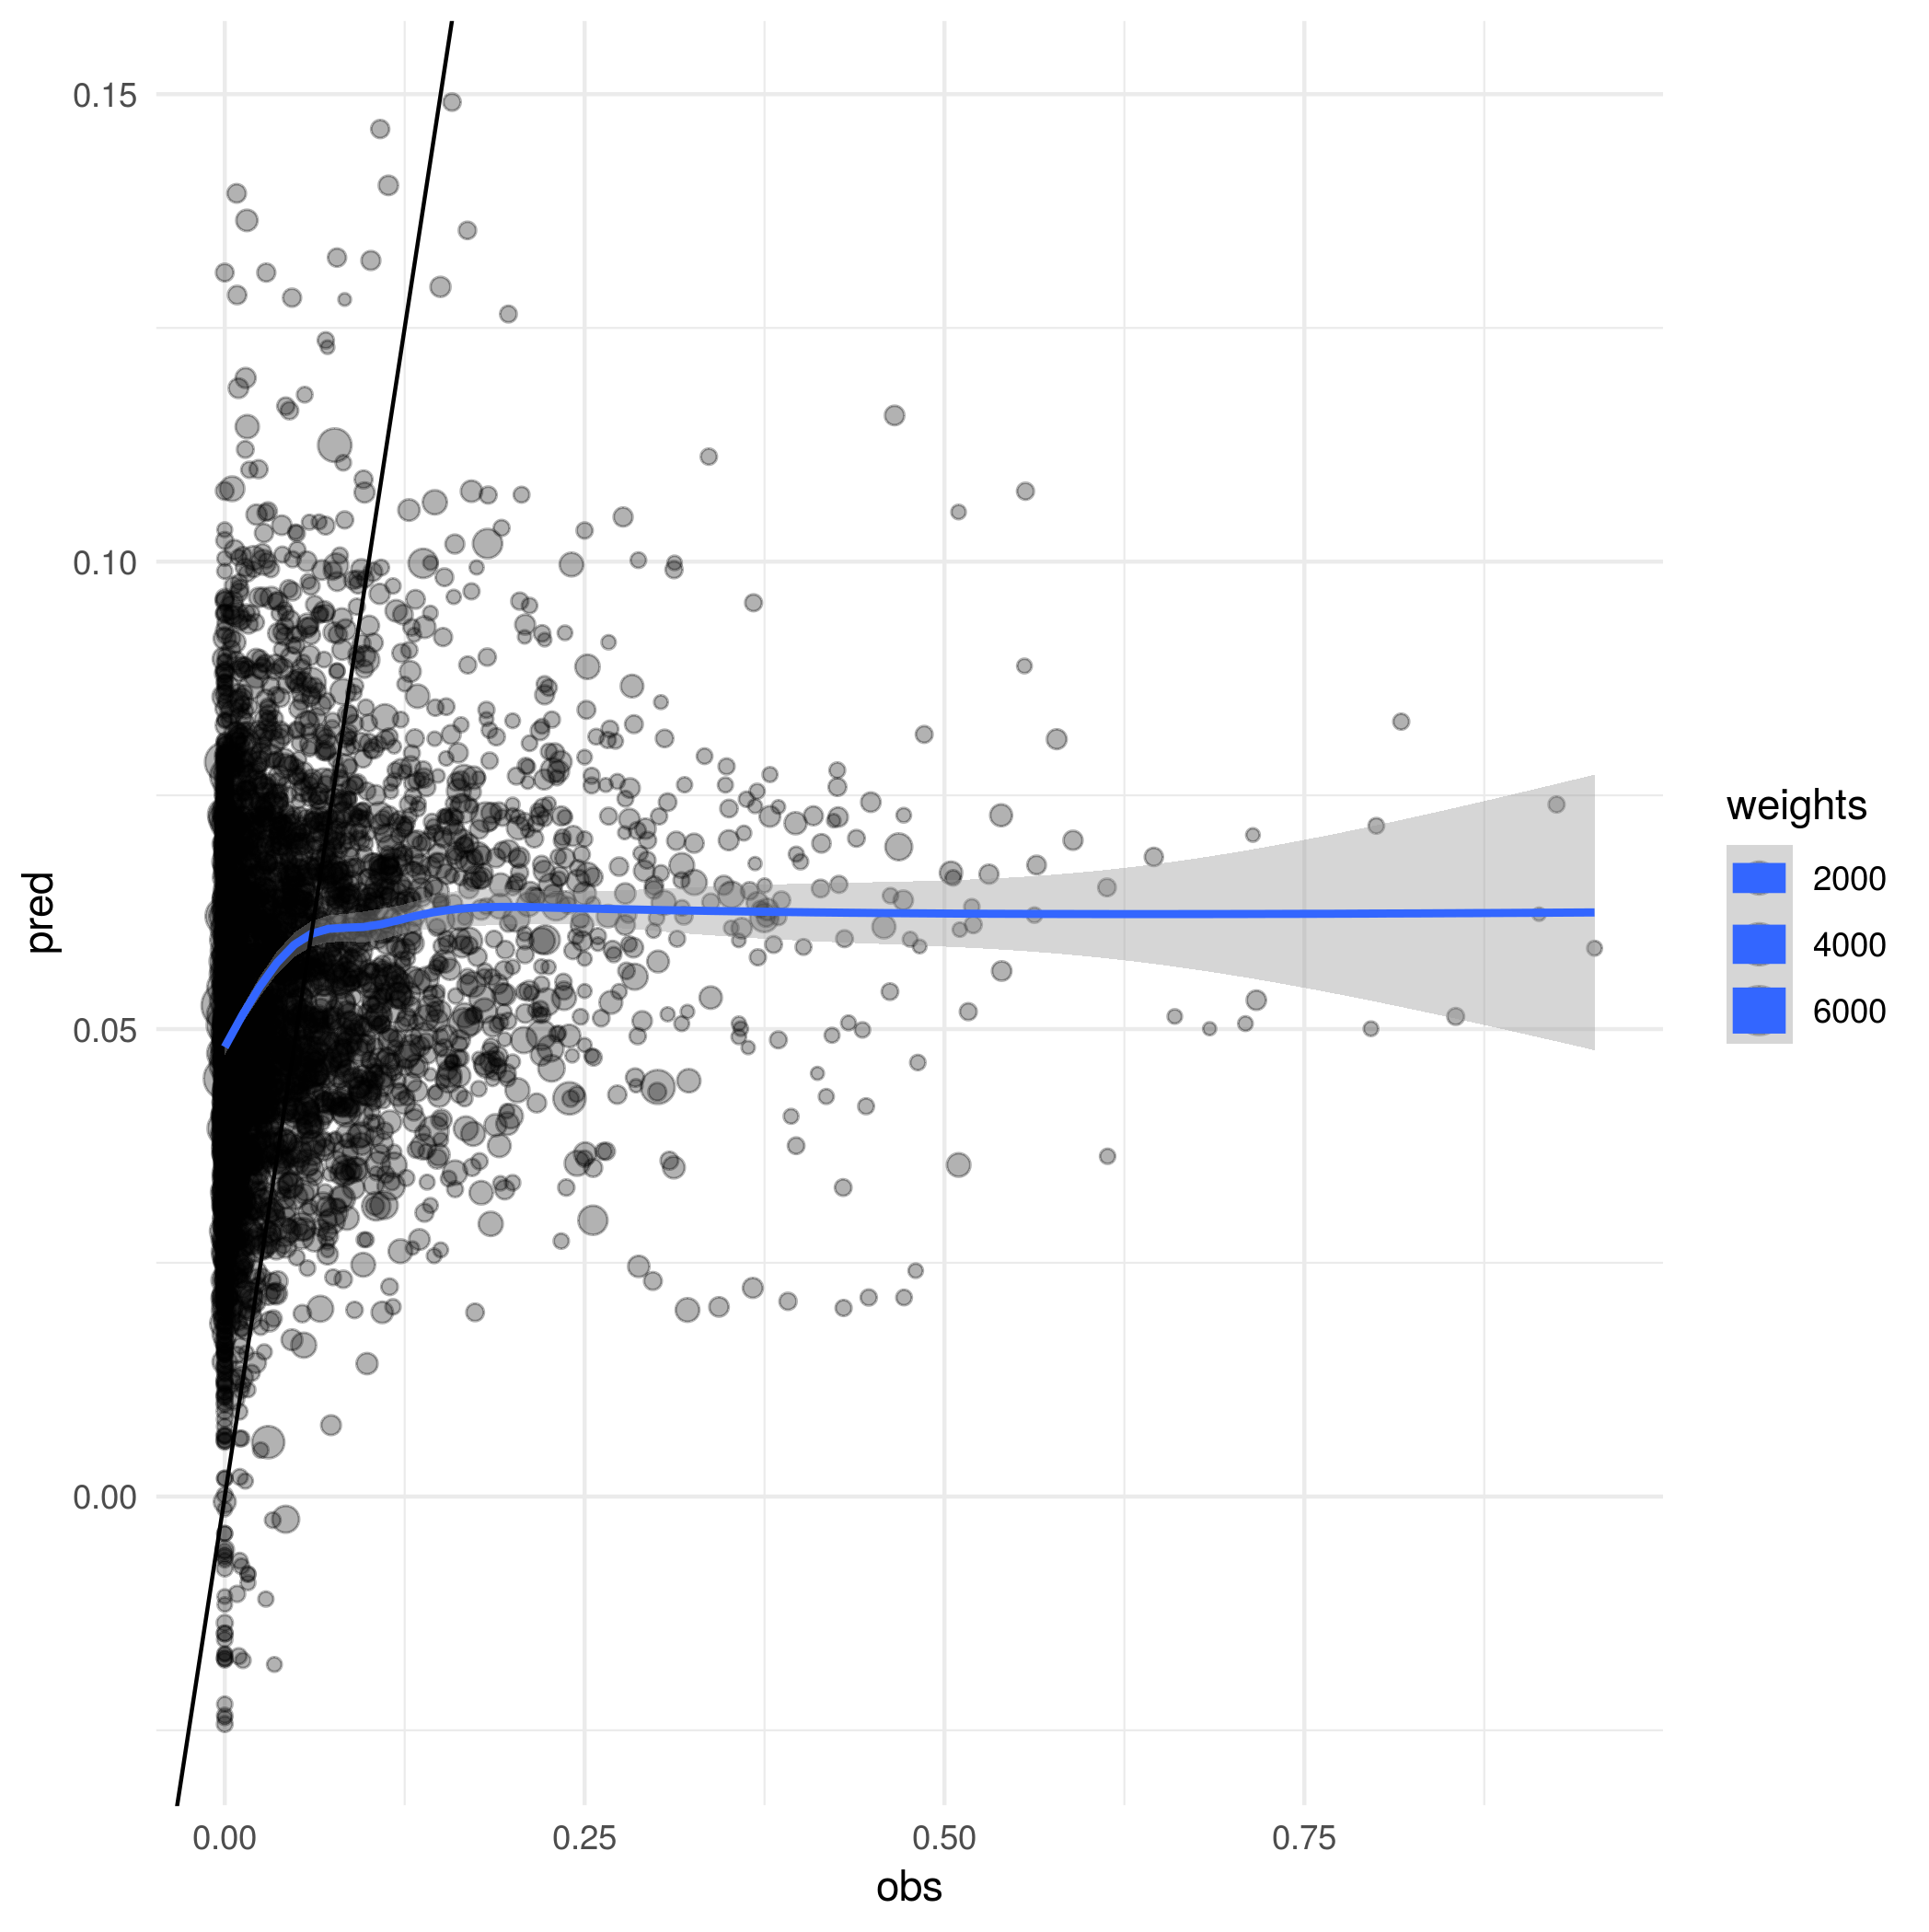
\includegraphics[width=0.6\textwidth]{figs/SI/enet_obspred_idn.png}
\caption{
  Scatter plot of predictions and held out observed data for the elastic net trained on the Indonesia dataset.
}

\end{figure}


\begin{figure}[h!]
  \centering
  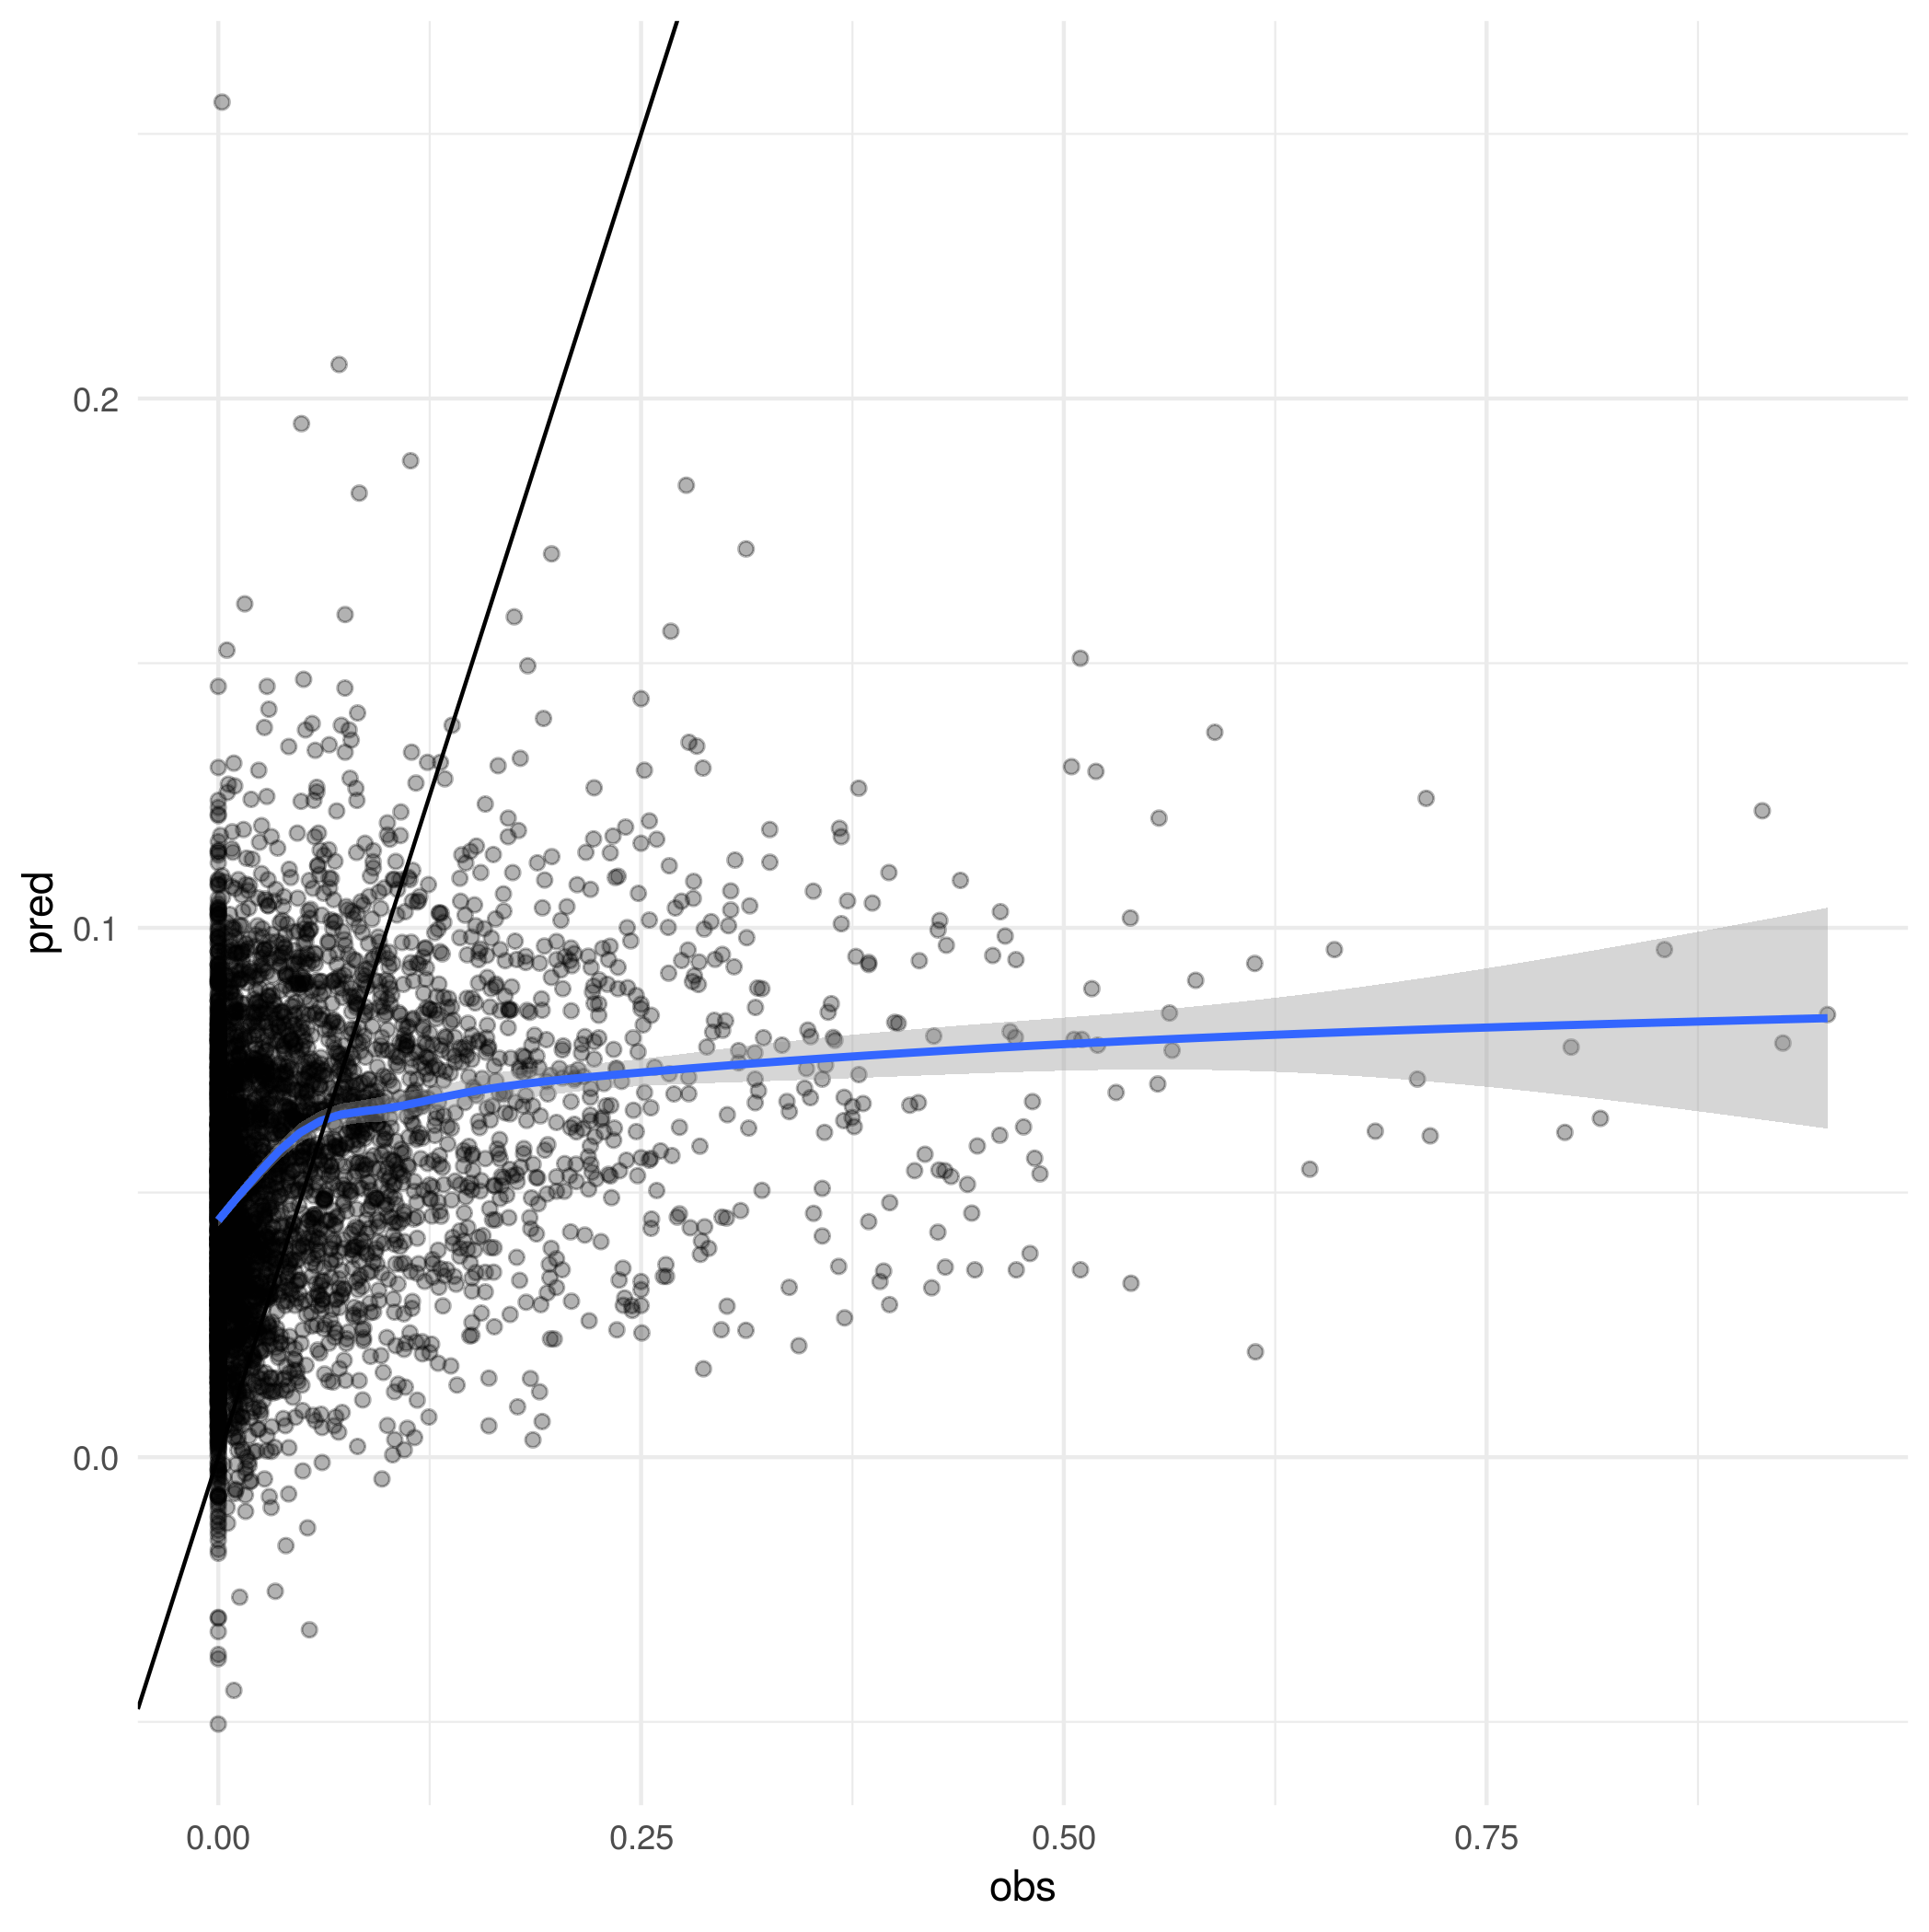
\includegraphics[width=0.6\textwidth]{figs/SI/ppr_obspred_idn.png}
\caption{
  Scatter plot of predictions and held out observed data for the PPR trained on the Indonesia dataset.
}

\end{figure}


\begin{figure}[h!]
  \centering
  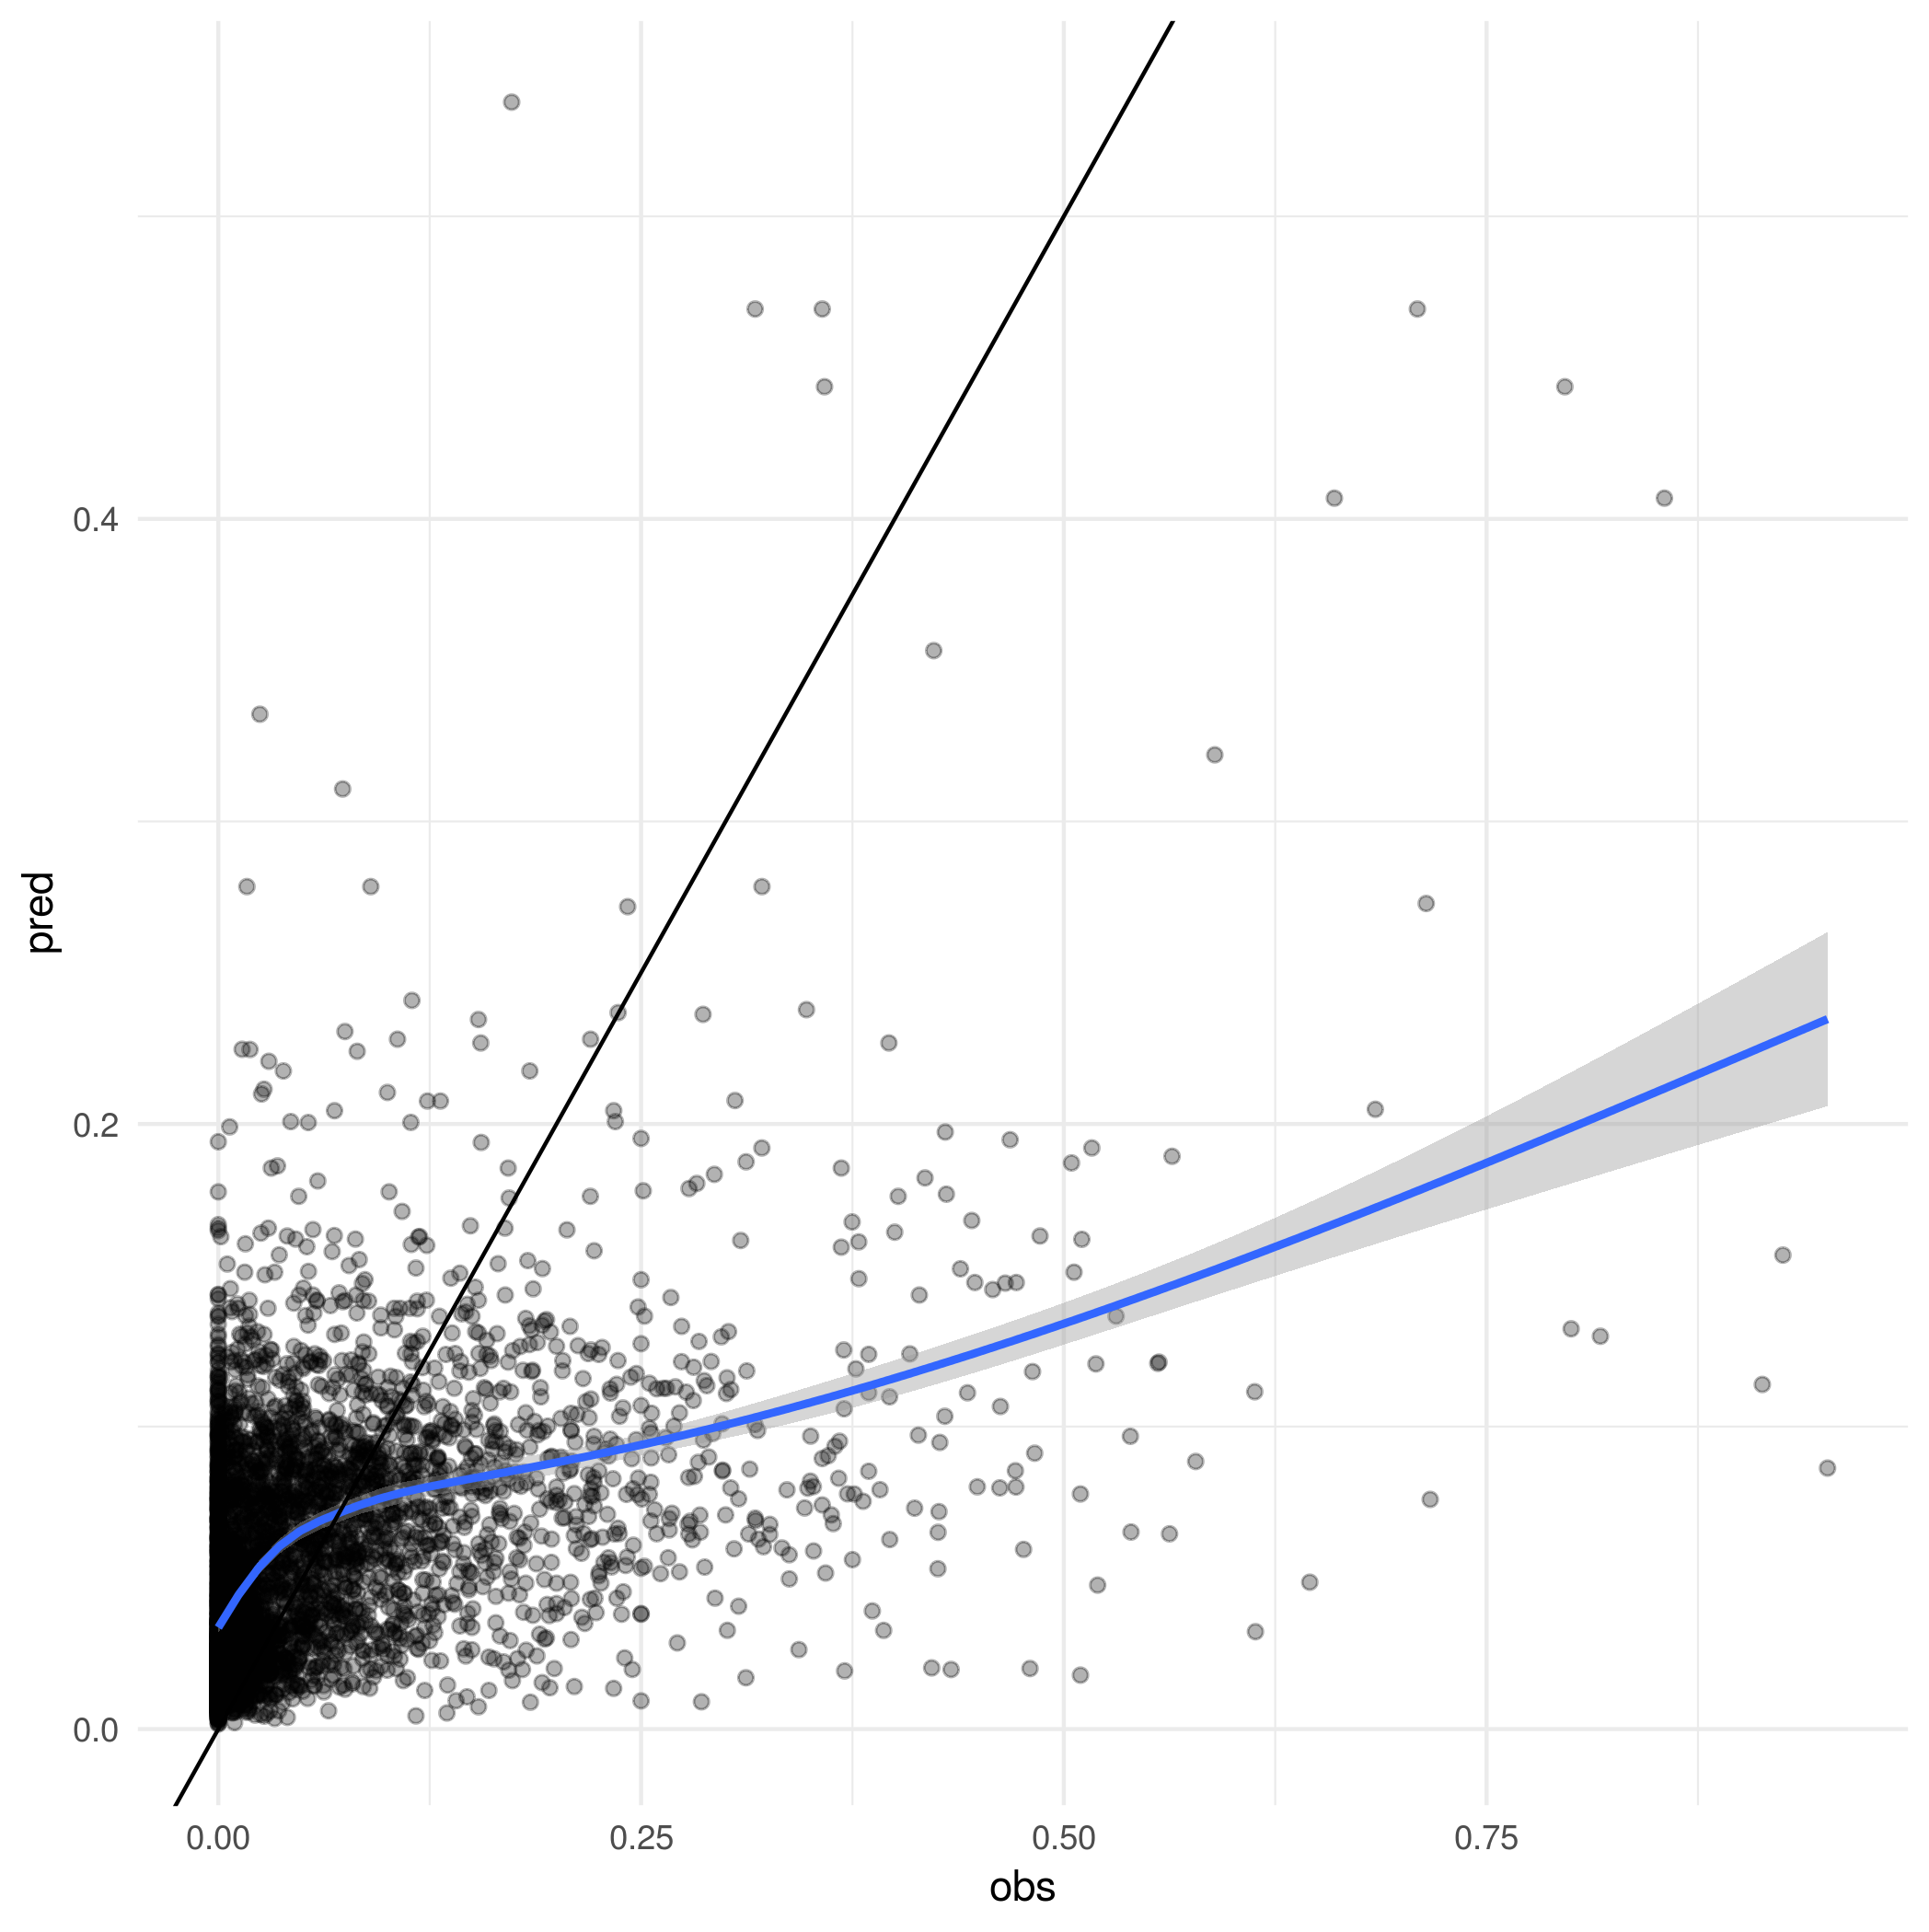
\includegraphics[width=0.6\textwidth]{figs/SI/ranger_obspred_idn.png}
\caption{
  Scatter plot of predictions and held out observed data for the Random Forest trained on the Indonesia dataset.
}

\end{figure}


\begin{figure}[h!]
  \centering
  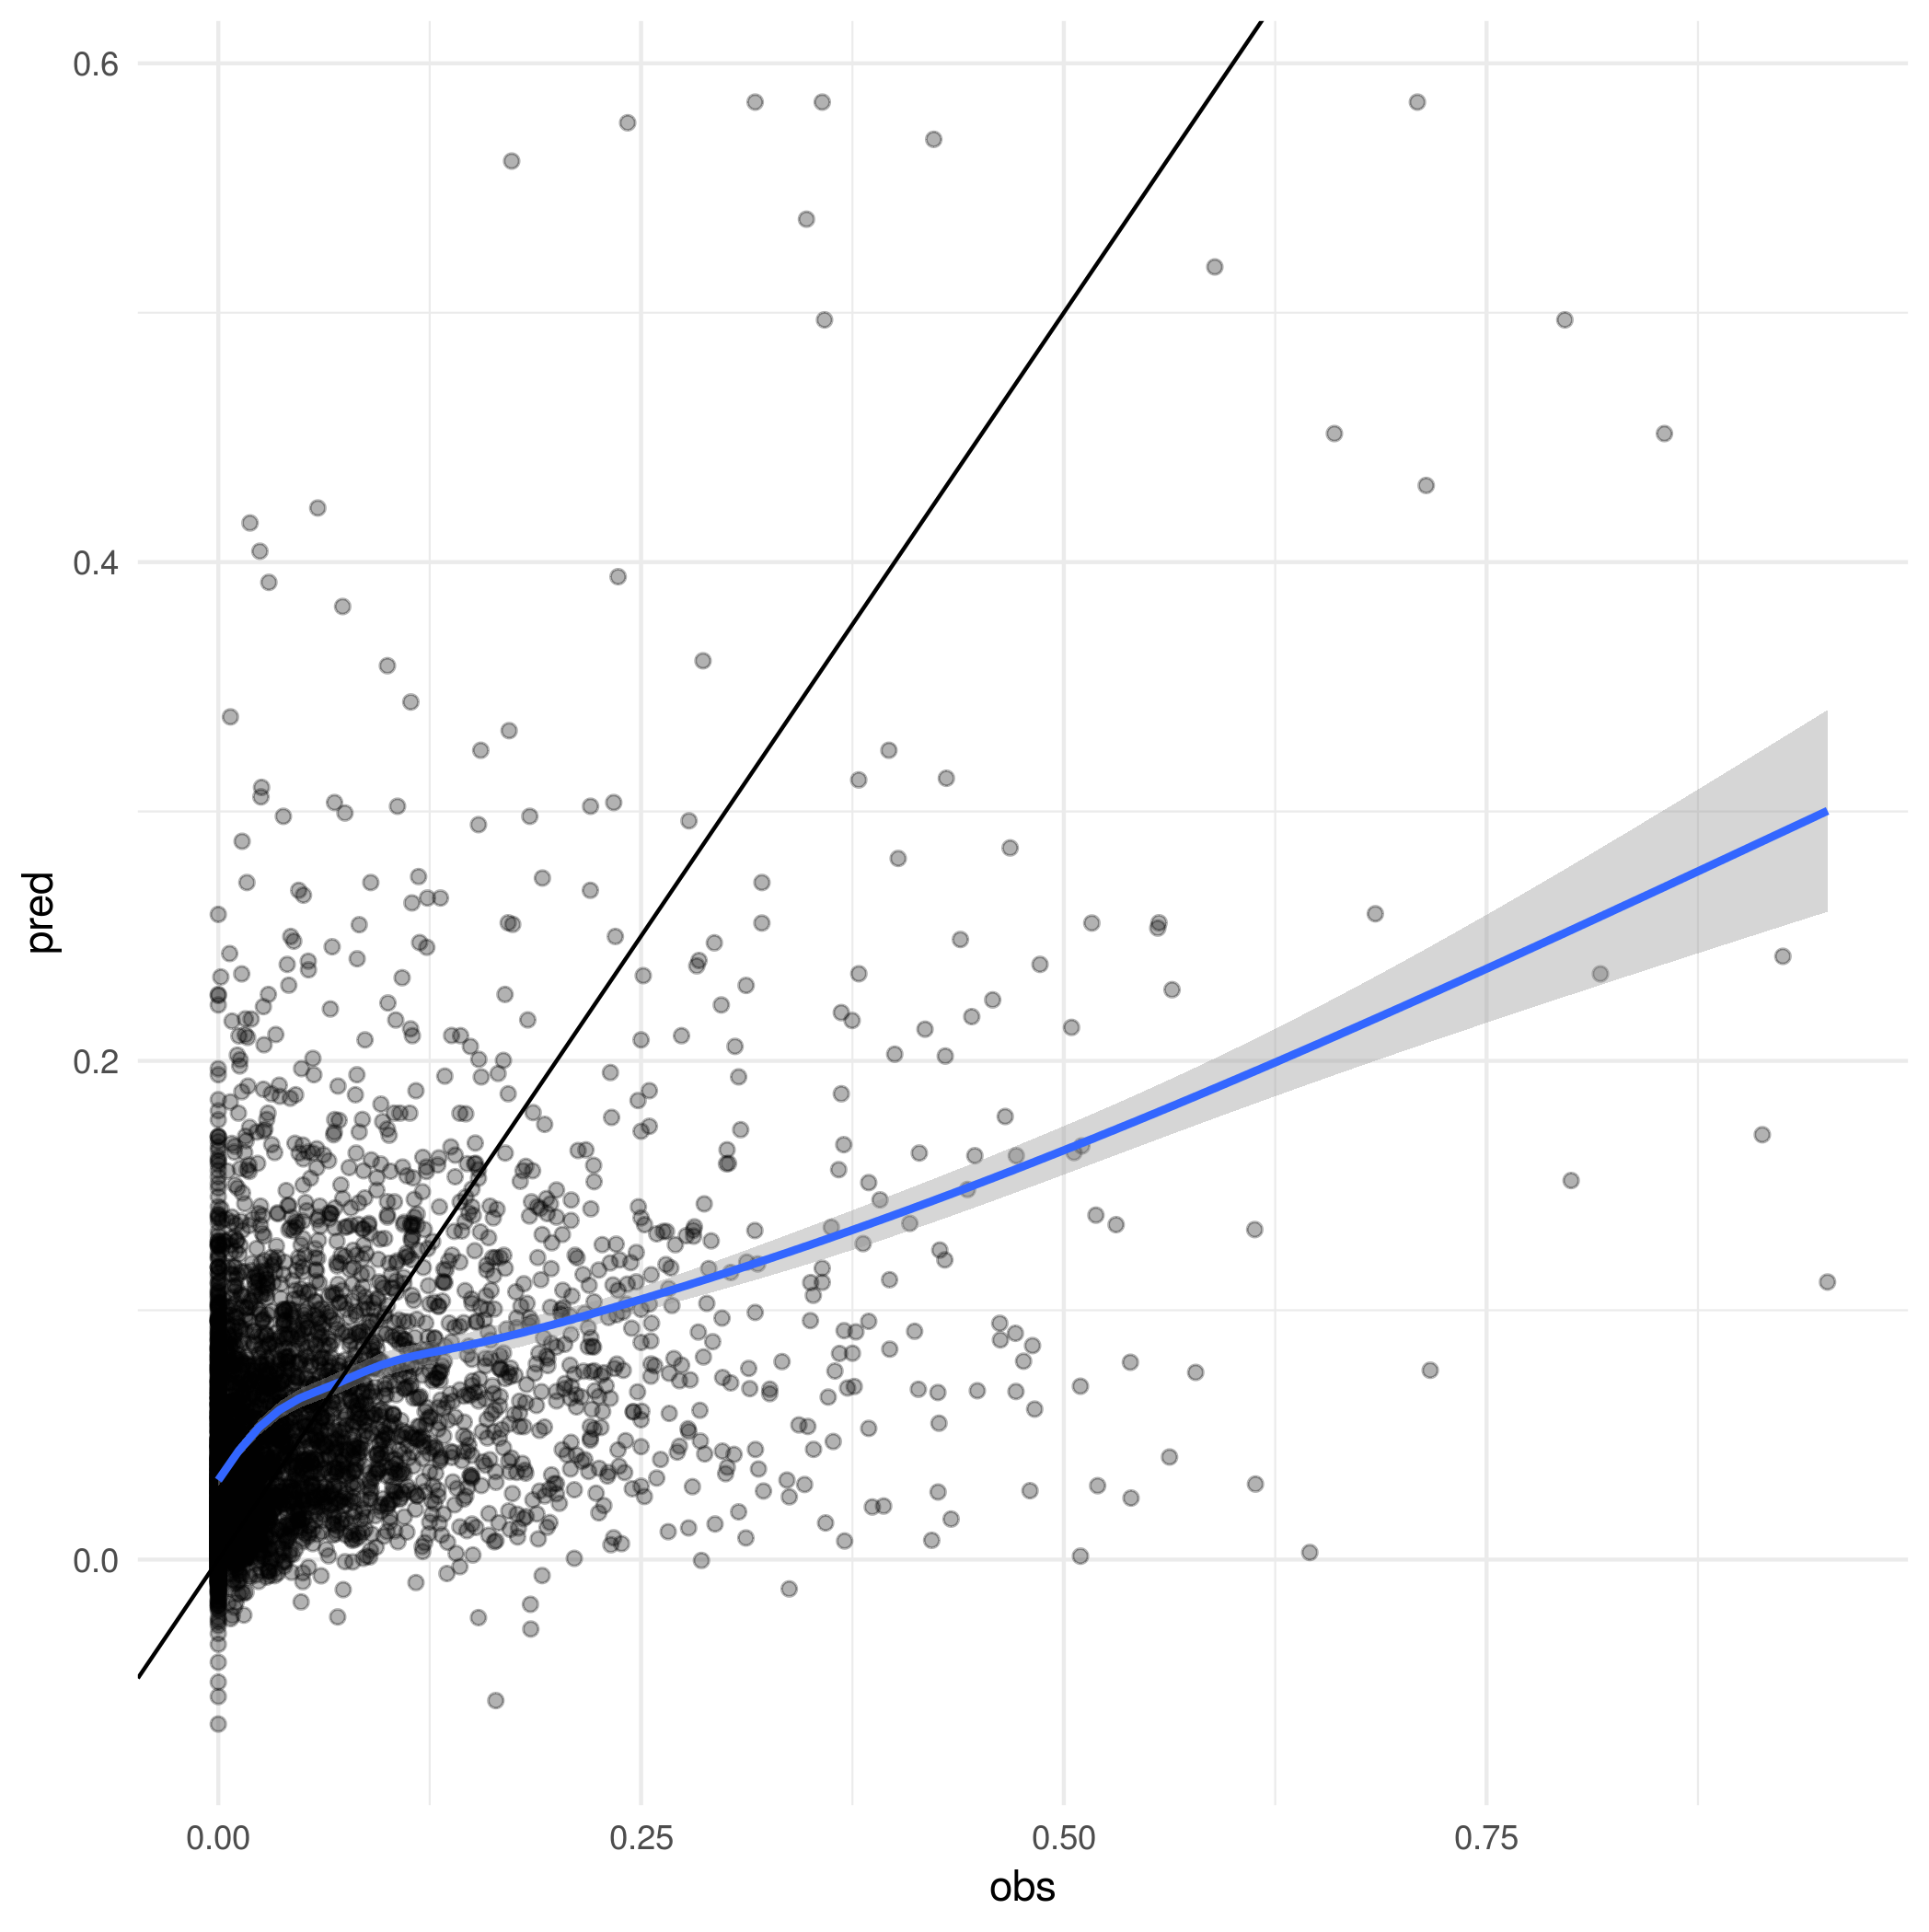
\includegraphics[width=0.6\textwidth]{figs/SI/xgboost_obspred_idn.png}
\caption{
  Scatter plot of predictions and held out observed data for the GBM trained on the Indonesia dataset.
}

\end{figure}


\clearpage
\subsection{Hyperparameter optimisation}

As ranger and GBM were tuned with random hyperparameter search, the plots become difficult and are not included.


\begin{figure}[h!]
  \centering
  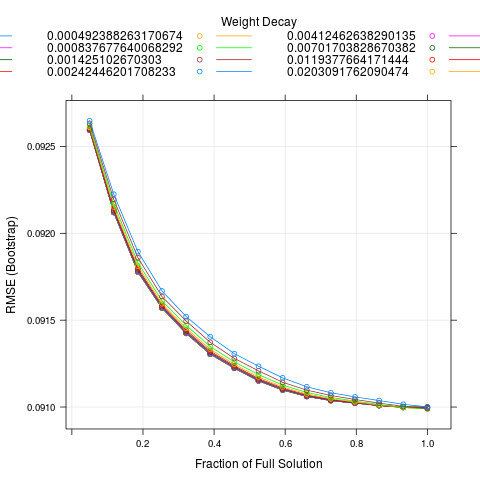
\includegraphics[width=0.6\textwidth]{figs/SI/enetopt_idn.png}
\caption{
  Optimisation for elastic net hyperparameters trained on the Indonesia dataset.
}
\end{figure}



\begin{figure}[h!]
  \centering
  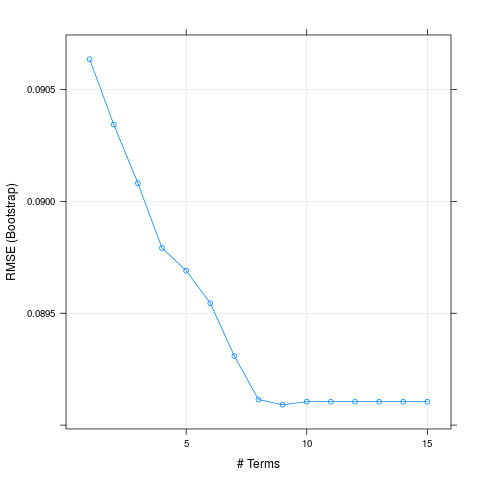
\includegraphics[width=0.6\textwidth]{figs/SI/ppropt_idn.png}
\caption{
  Optimisation for PPR hyperparameters trained on the Indonesia dataset.
}

\end{figure}






\clearpage
%%%%%%%%%%%%%%%%%%%%%%%%%%%%%%%%%%%%%%%%%%%%%%%%%%%%%%%%%%%%%%%%%%%%%%%
\section{Madagascar dataset Machine Learning}
%%%%%%%%%%%%%%%%%%%%%%%%%%%%%%%%%%%%%%%%%%%%%%%%%%%%%%%%%%%%%%%%%%%%%%%





\subsection{Predictions}

\begin{figure}[h!]
  \centering
  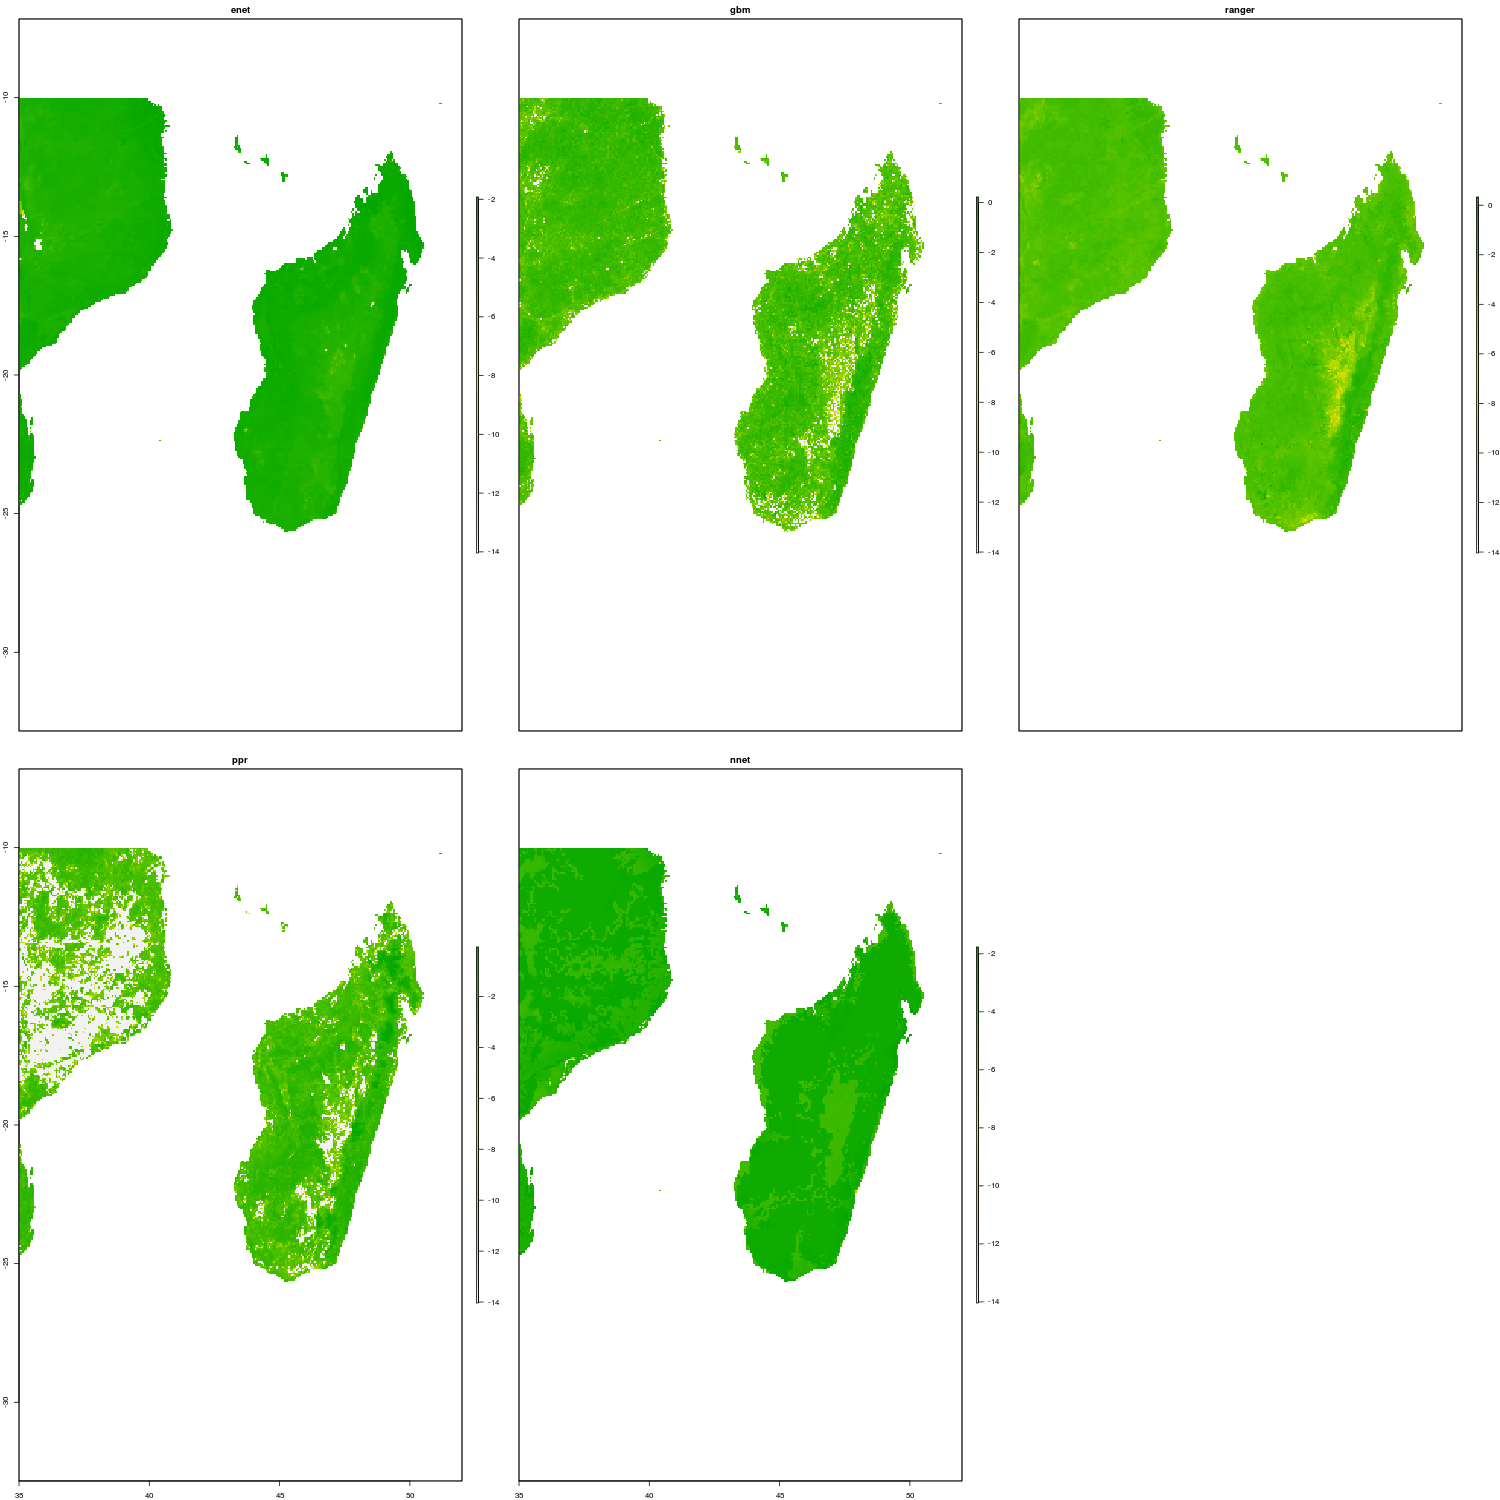
\includegraphics[width=1\textwidth]{figs/SI/MDG_all_ml.png}
\caption{
  Predictions from machine learning models trained on Malagasy prevalence data.
}

\end{figure}


\begin{figure}[h!]
  \centering
  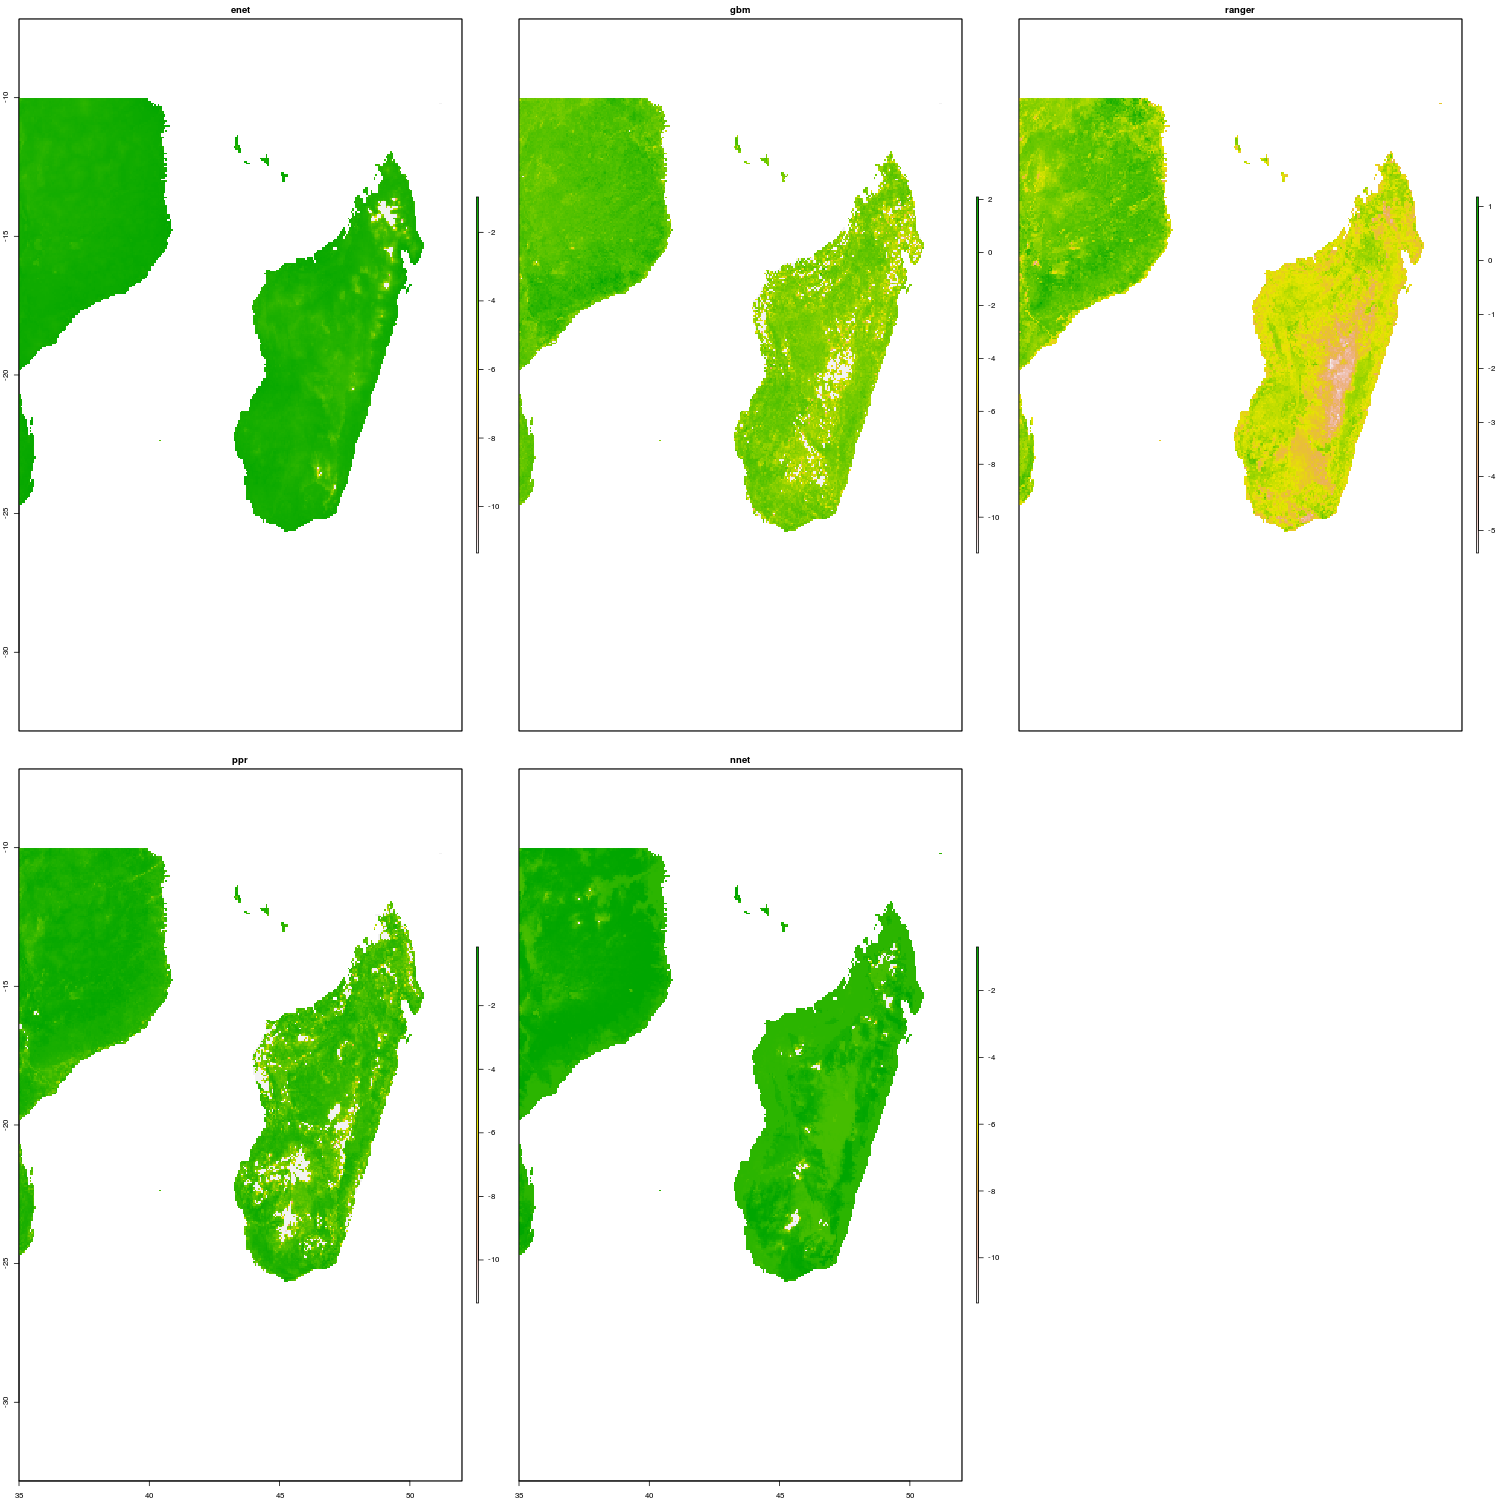
\includegraphics[width=1\textwidth]{figs/SI/MDG_all_globalml.png}
\caption{
  Predictions over Madagascar from machine learning models trained on global prevalence data.
}

\end{figure}




\clearpage
\subsection{Out-of-MDGmple scatter plots}


\begin{figure}[h!]
  \centering
  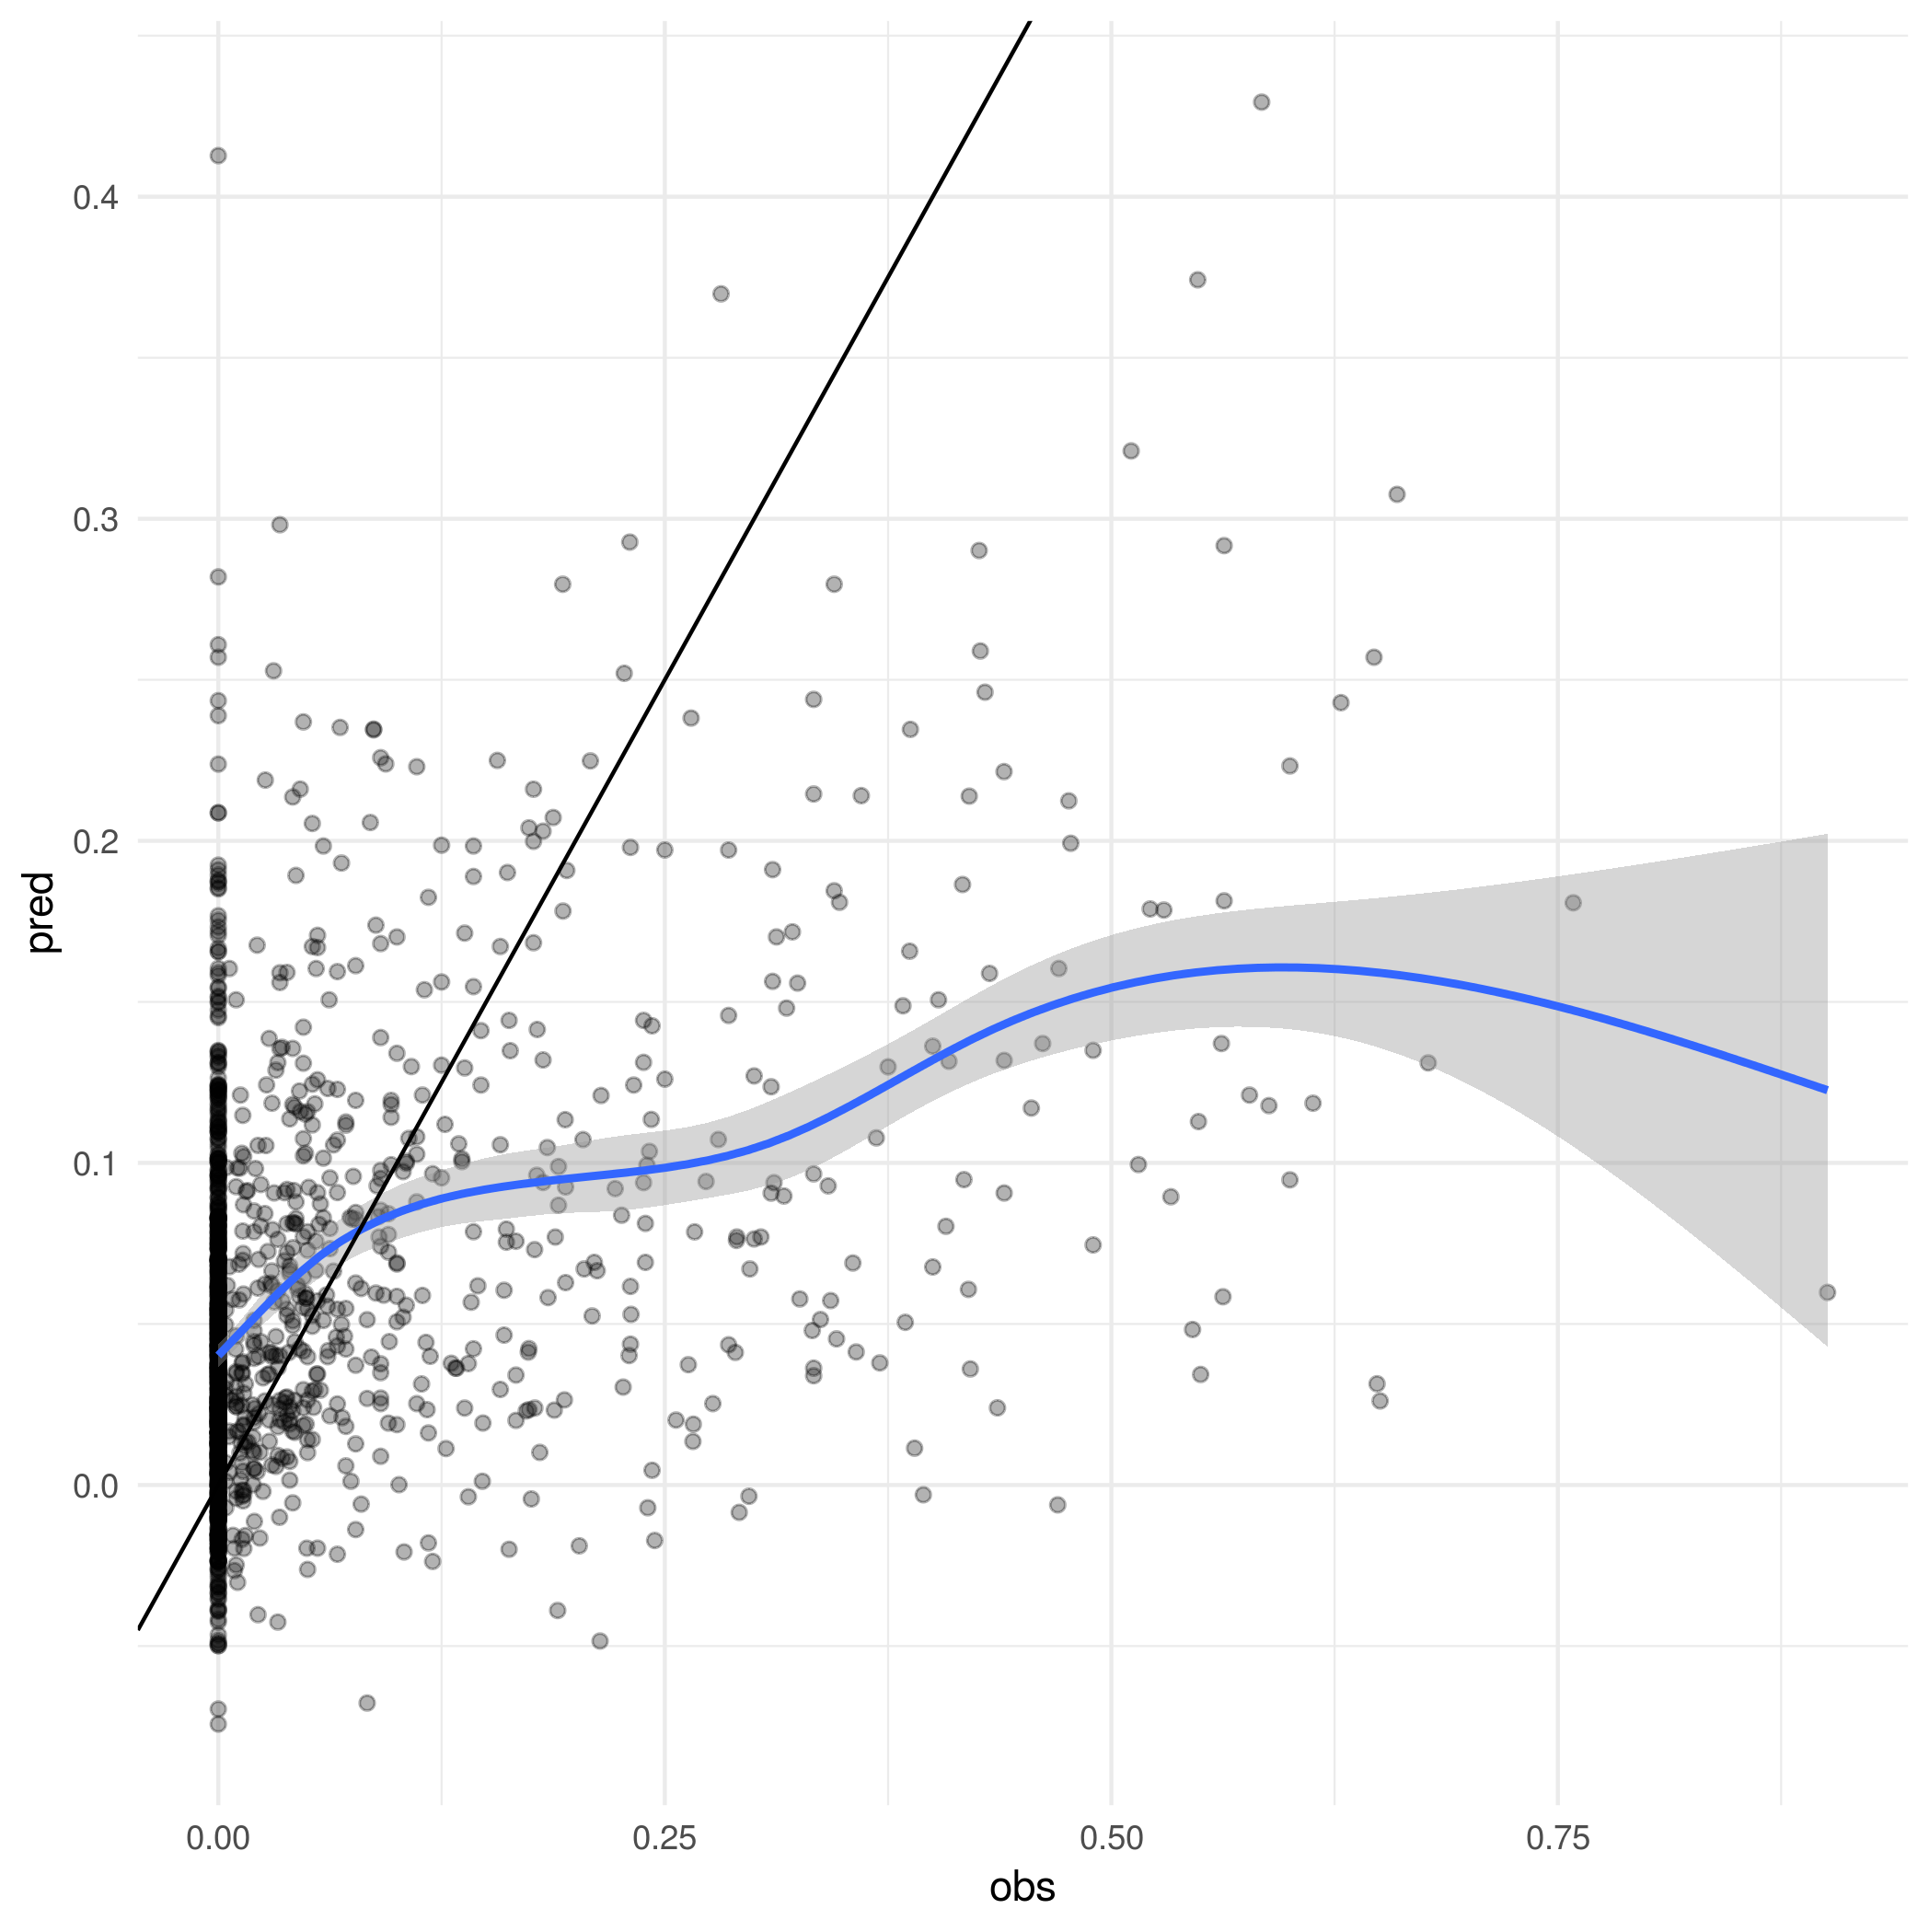
\includegraphics[width=0.6\textwidth]{figs/SI/nnet_obspred_mdg.png}
\caption{
  Scatter plot of predictions and held out observed data for the neural network trained on the Madagascar dataset.
}

\end{figure}



\begin{figure}[h!]
  \centering
  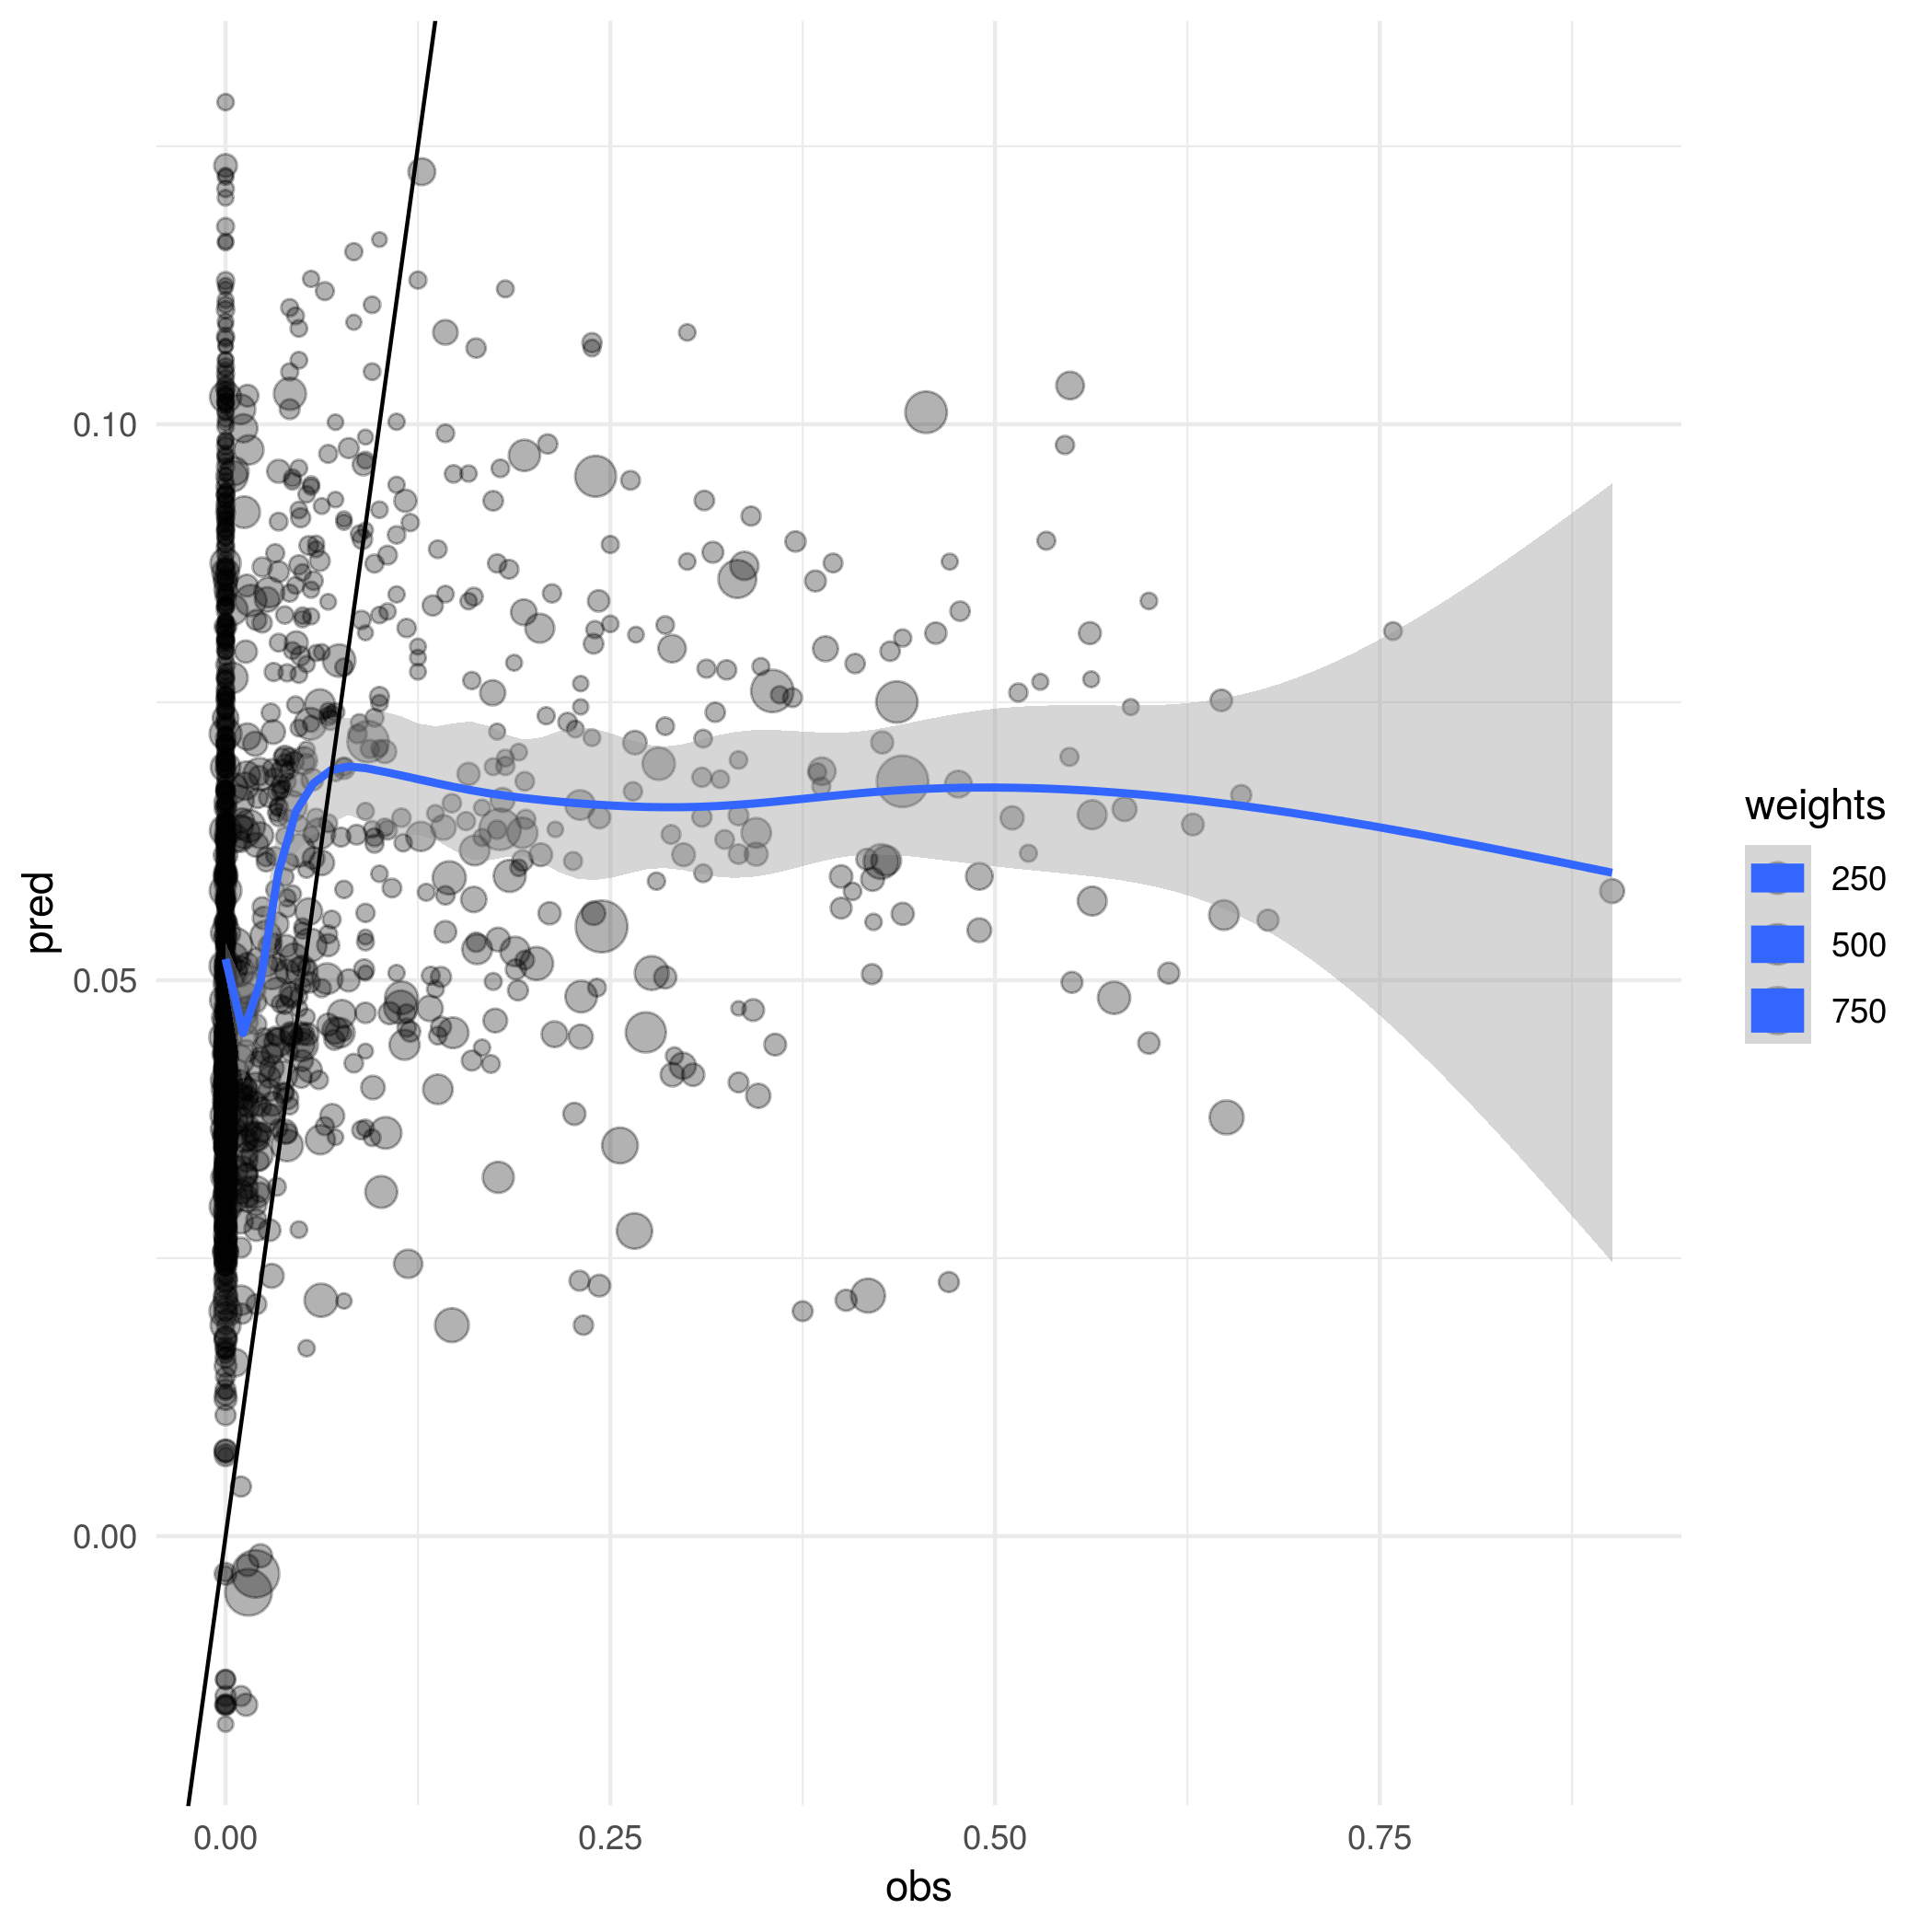
\includegraphics[width=0.6\textwidth]{figs/SI/enet_obspred_mdg.png}
\caption{
  Scatter plot of predictions and held out observed data for the elastic net trained on the Madagascar dataset.
}

\end{figure}


\begin{figure}[h!]
  \centering
  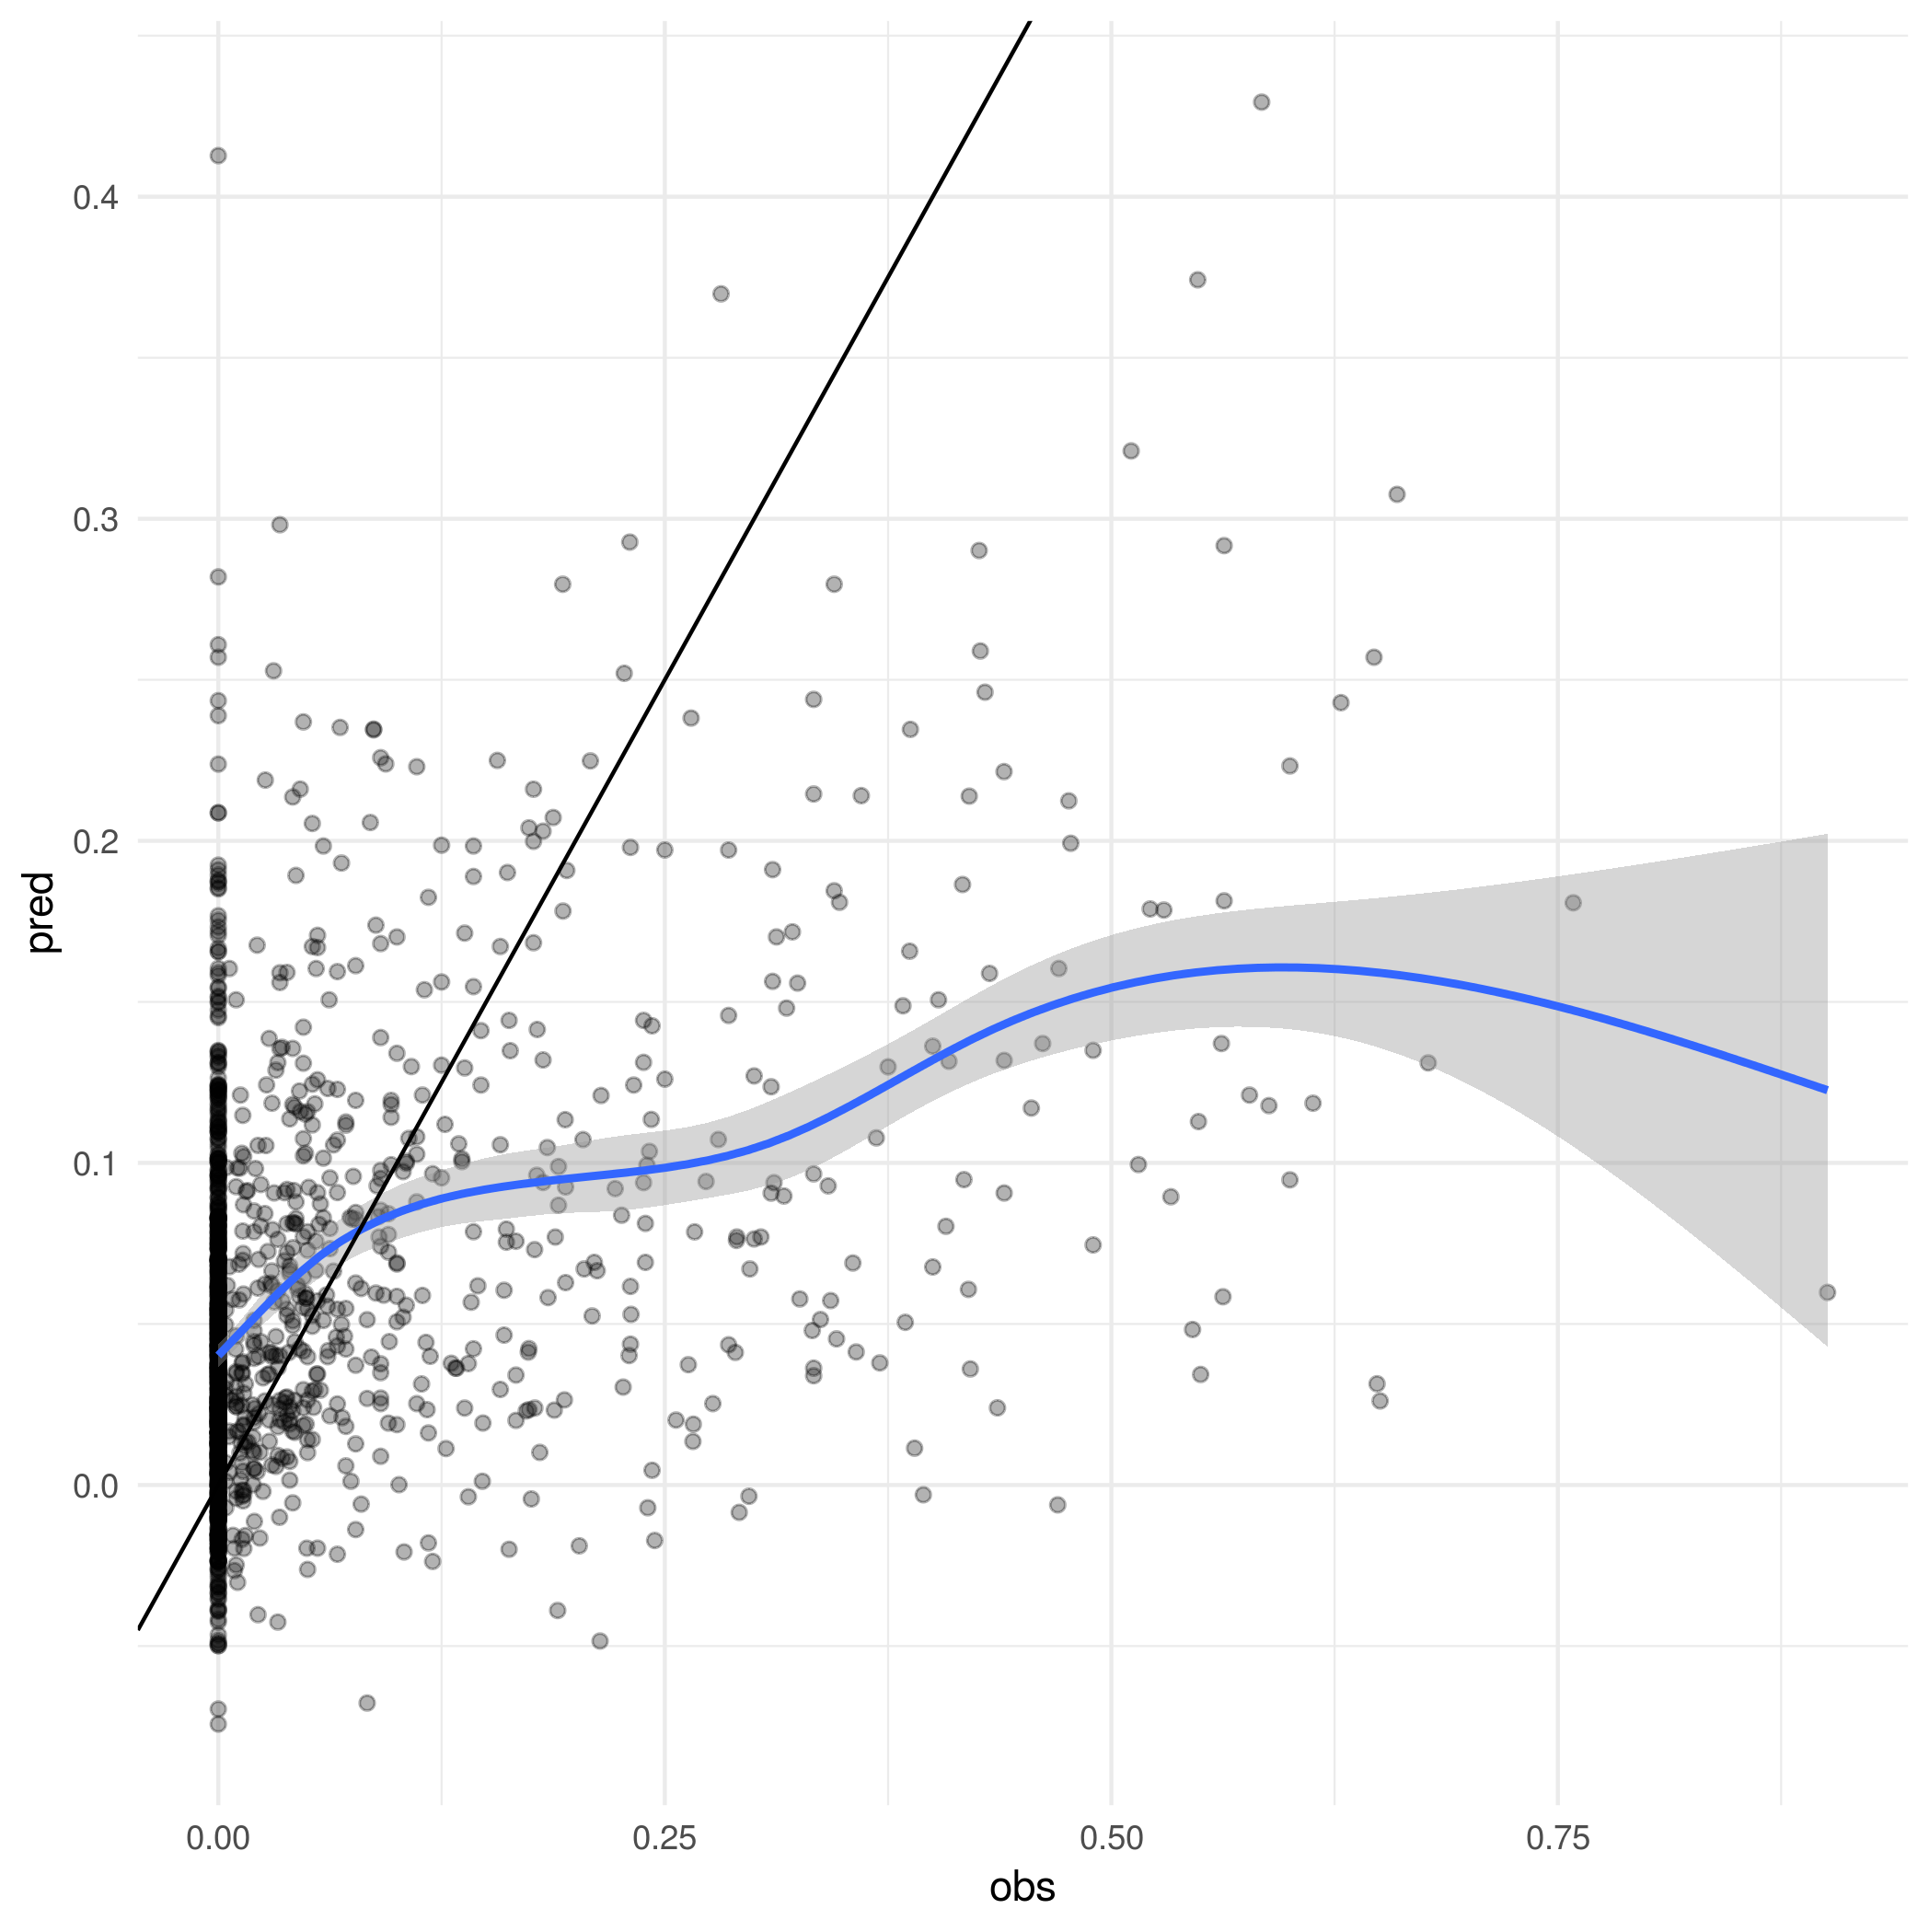
\includegraphics[width=0.6\textwidth]{figs/SI/ppr_obspred_mdg.png}
\caption{
  Scatter plot of predictions and held out observed data for the PPR trained on the Madagascar dataset.
}

\end{figure}


\begin{figure}[h!]
  \centering
  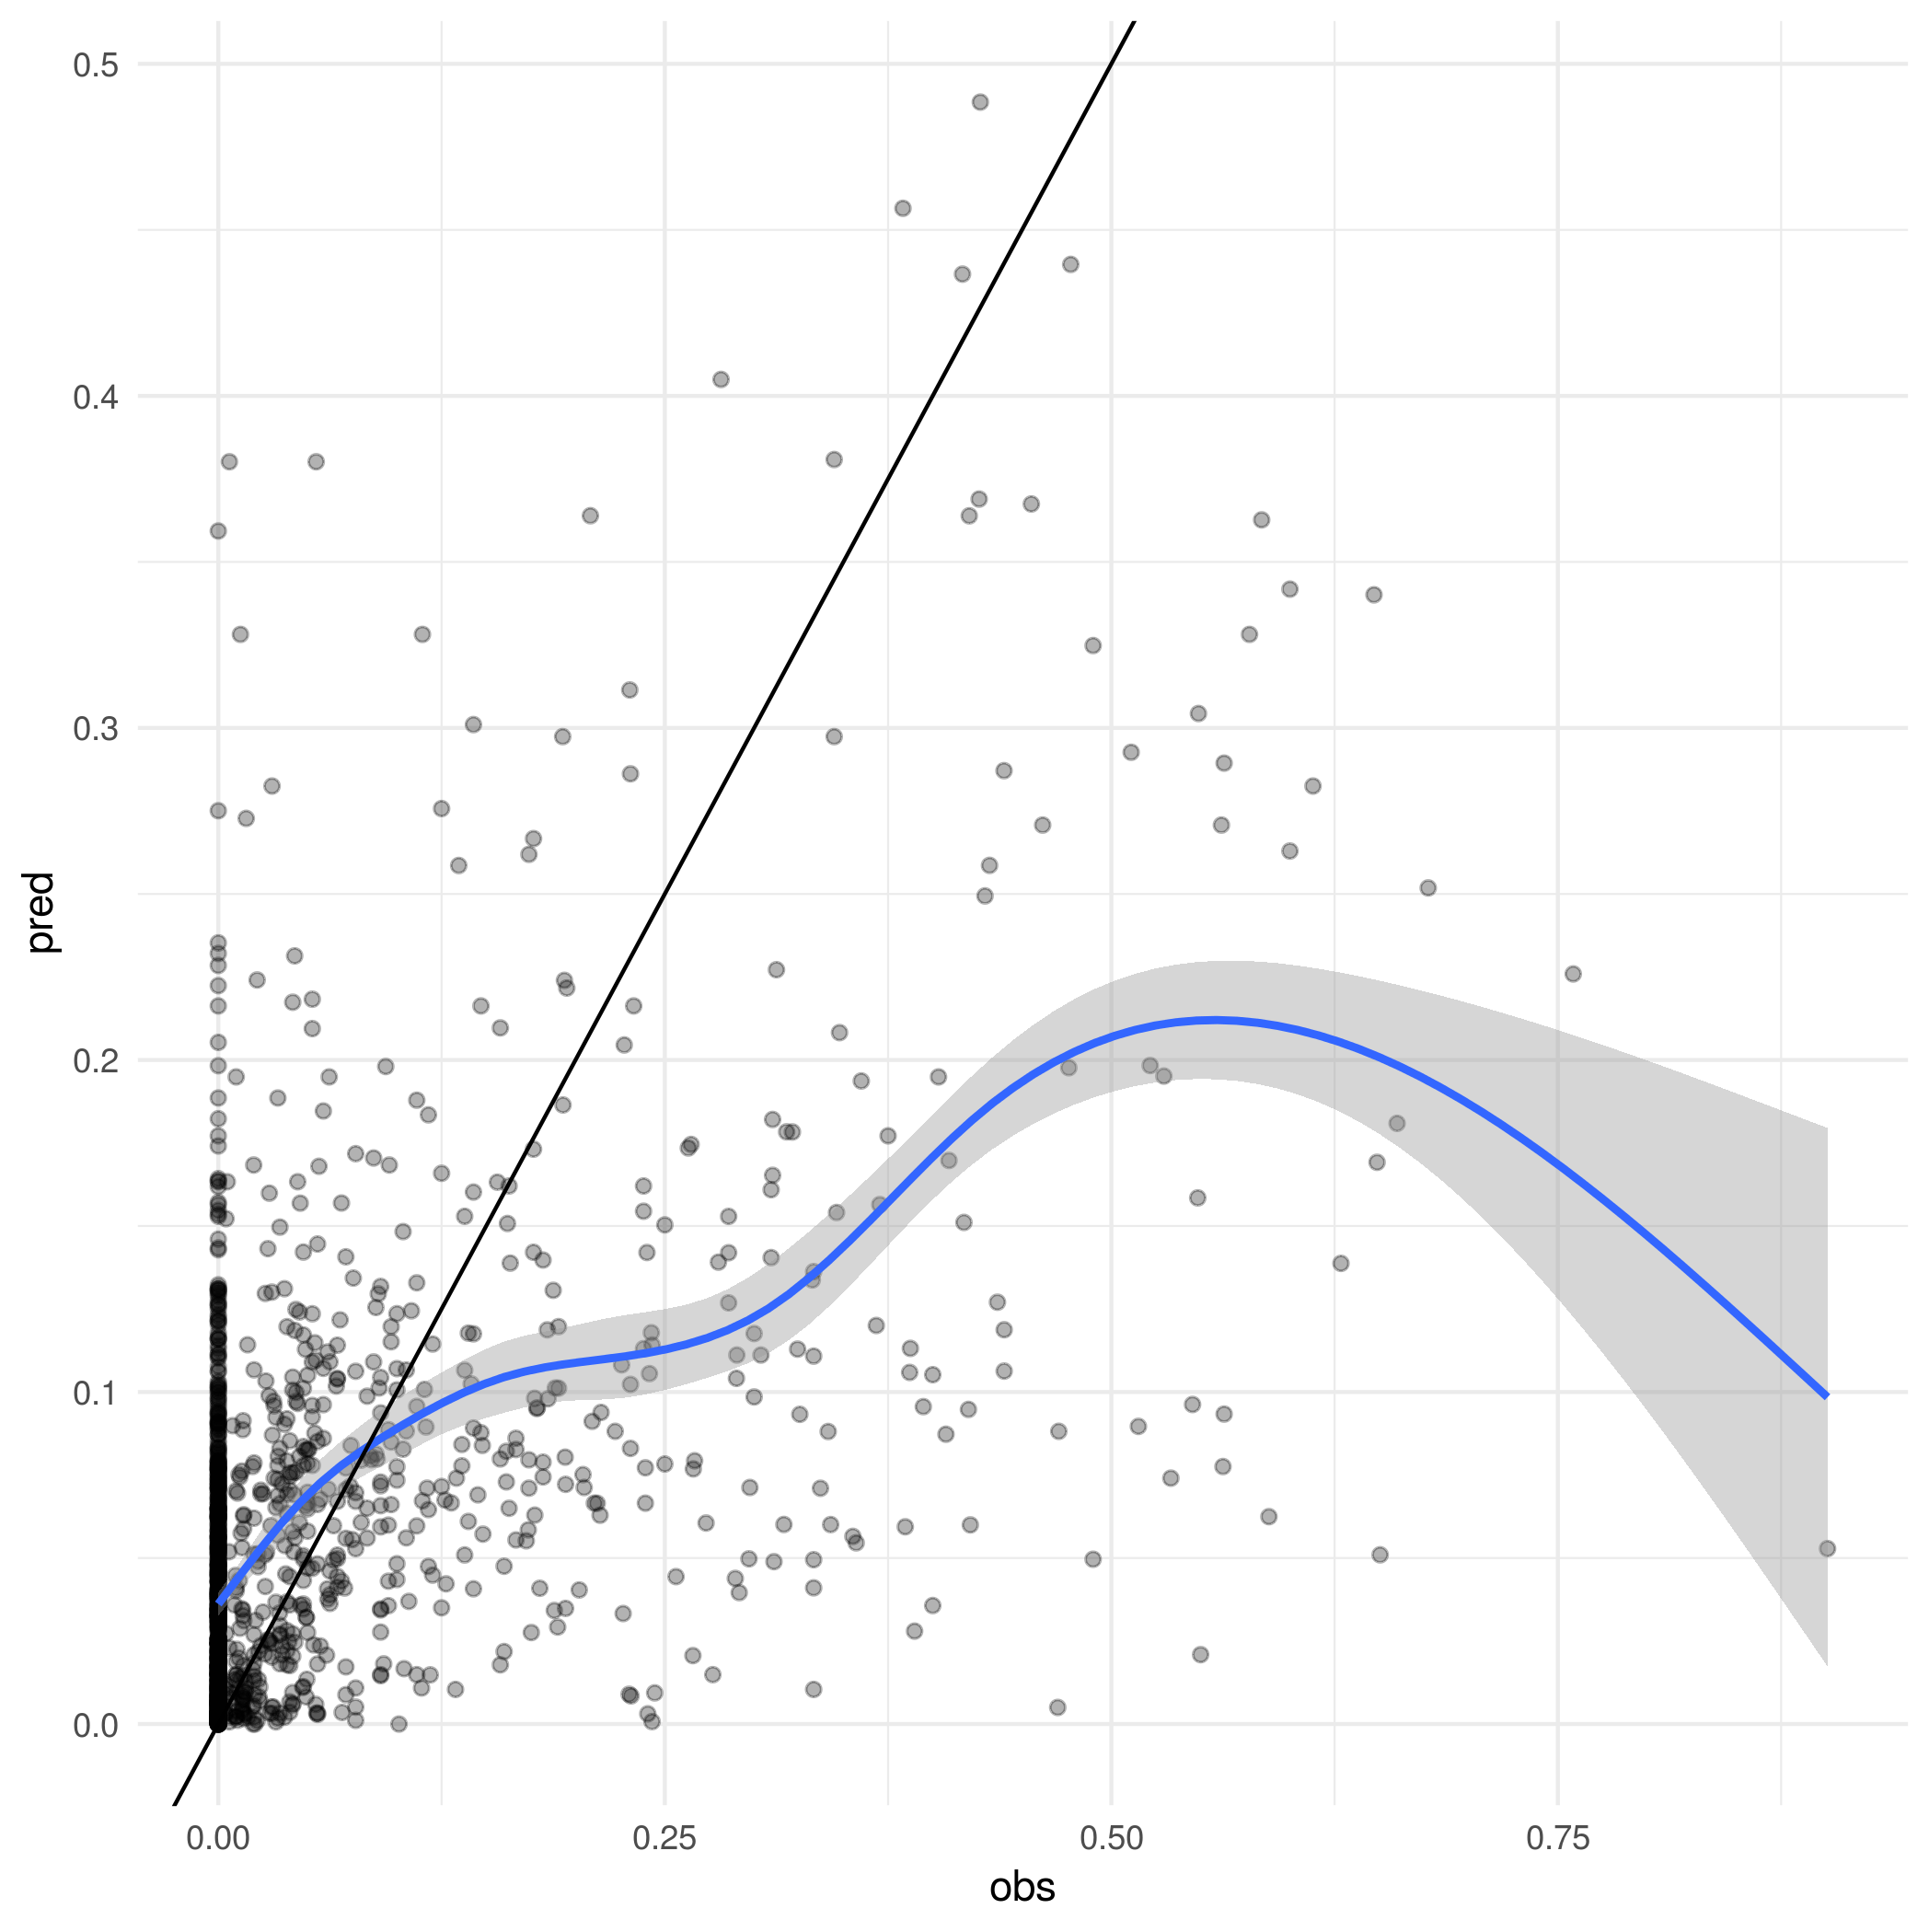
\includegraphics[width=0.6\textwidth]{figs/SI/ranger_obspred_mdg.png}
\caption{
  Scatter plot of predictions and held out observed data for the Random Forest trained on the Madagascar dataset.
}

\end{figure}


\begin{figure}[h!]
  \centering
  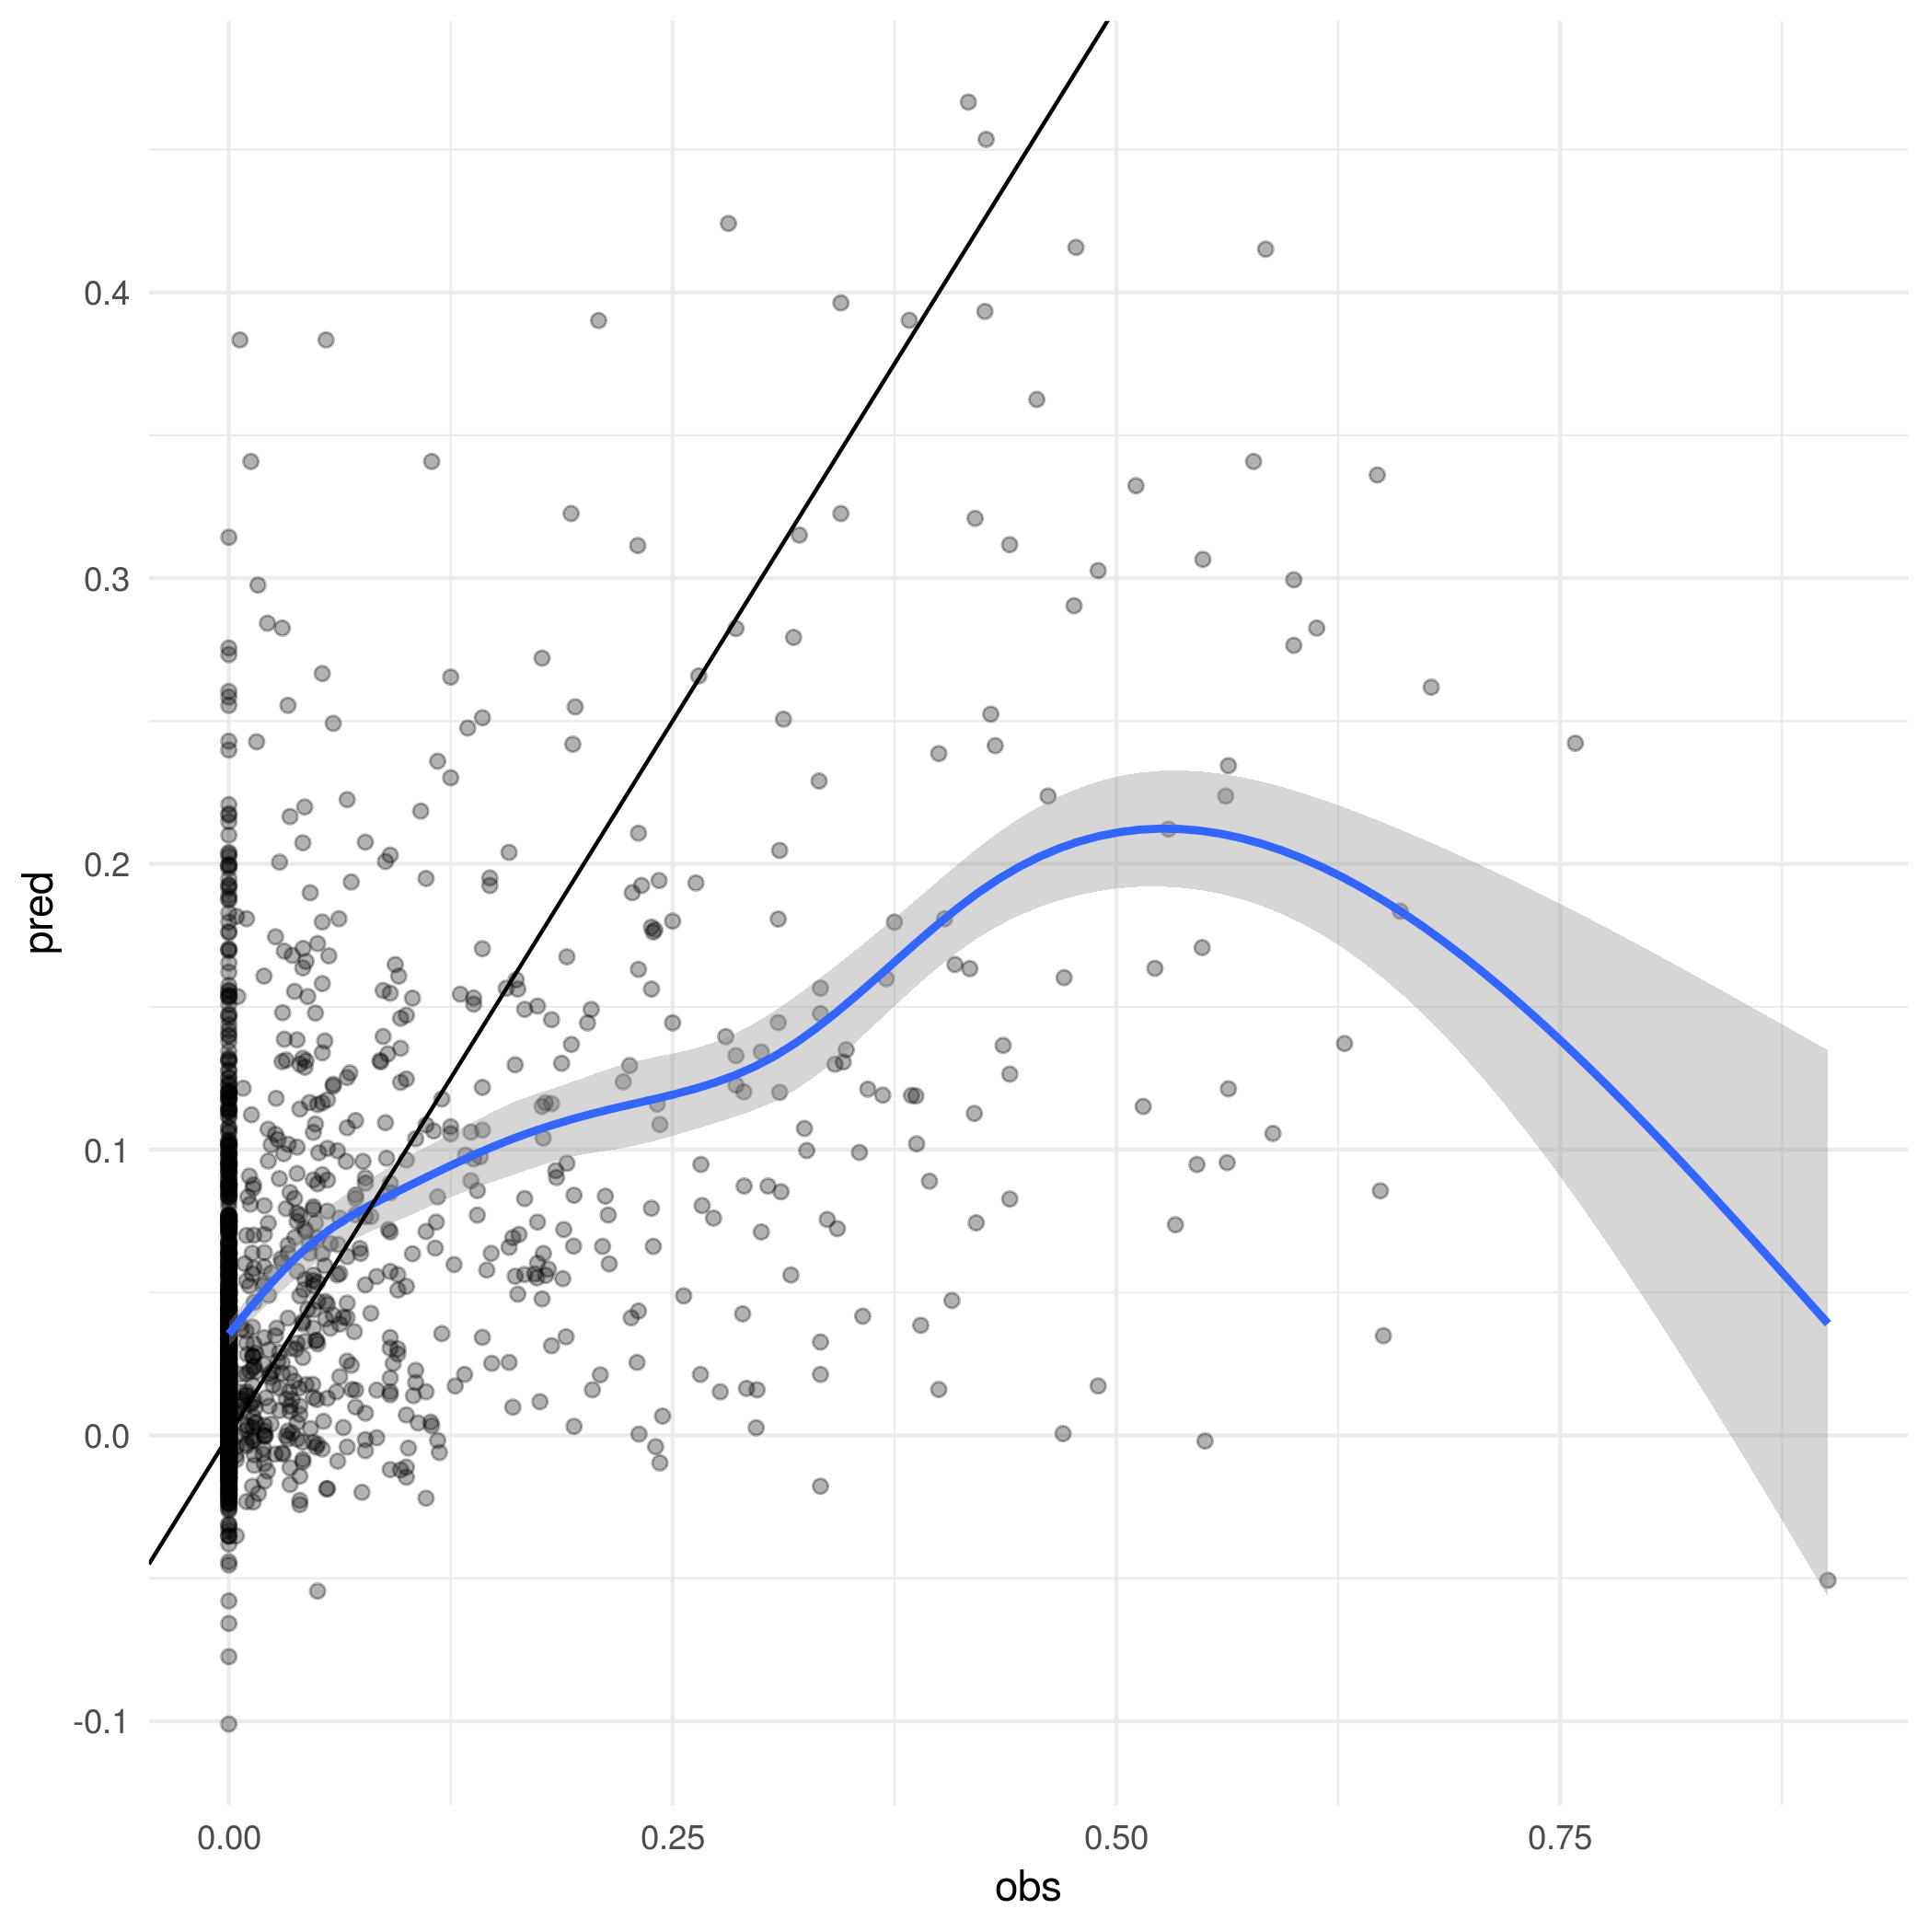
\includegraphics[width=0.6\textwidth]{figs/SI/xgboost_obspred_mdg.png}
\caption{
  Scatter plot of predictions and held out observed data for the GBM trained on the Madagascar dataset.
}

\end{figure}


\clearpage
\subsection{Hyperparameter optimiMDGtion}

As ranger and GBM were tuned with random hyperparameter search, the plots become difficult and are not included.


\begin{figure}[h!]
  \centering
  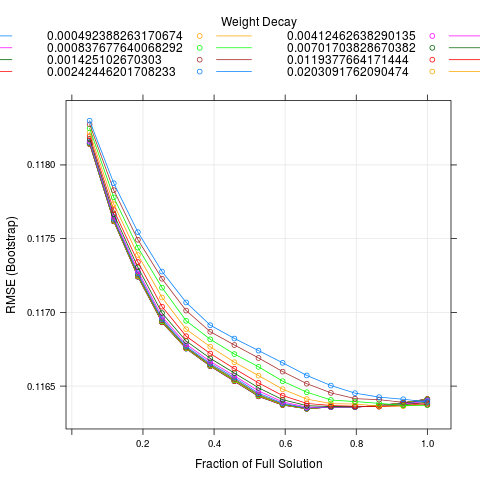
\includegraphics[width=0.6\textwidth]{figs/SI/enetopt_mdg.png}
\caption{
  OptimiMDGtion for elastic net hyperparameters trained on the Madagascar dataset.
}
\end{figure}



\begin{figure}[h!]
  \centering
  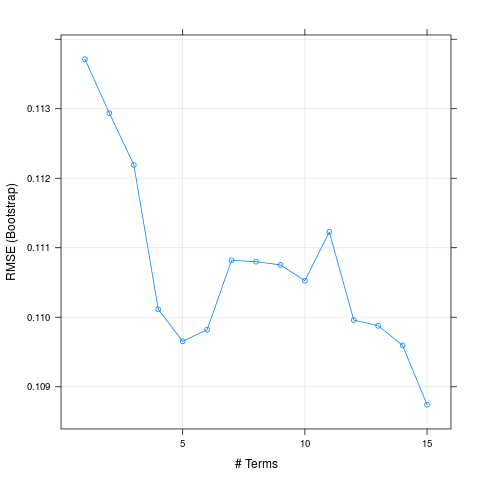
\includegraphics[width=0.6\textwidth]{figs/SI/ppropt_mdg.png}
\caption{
  OptimiMDGtion for PPR hyperparameters trained on the Madagascar dataset.
}

\end{figure}








\clearpage
%%%%%%%%%%%%%%%%%%%%%%%%%%%%%%%%%%%%%%%%%%%%%%%%%%%%%%%%%%%%%%%%%%%%%%%
\section{Senegal dataset Machine Learning}
%%%%%%%%%%%%%%%%%%%%%%%%%%%%%%%%%%%%%%%%%%%%%%%%%%%%%%%%%%%%%%%%%%%%%%%






\subsection{Predictions}

\begin{figure}[h!]
  \centering
  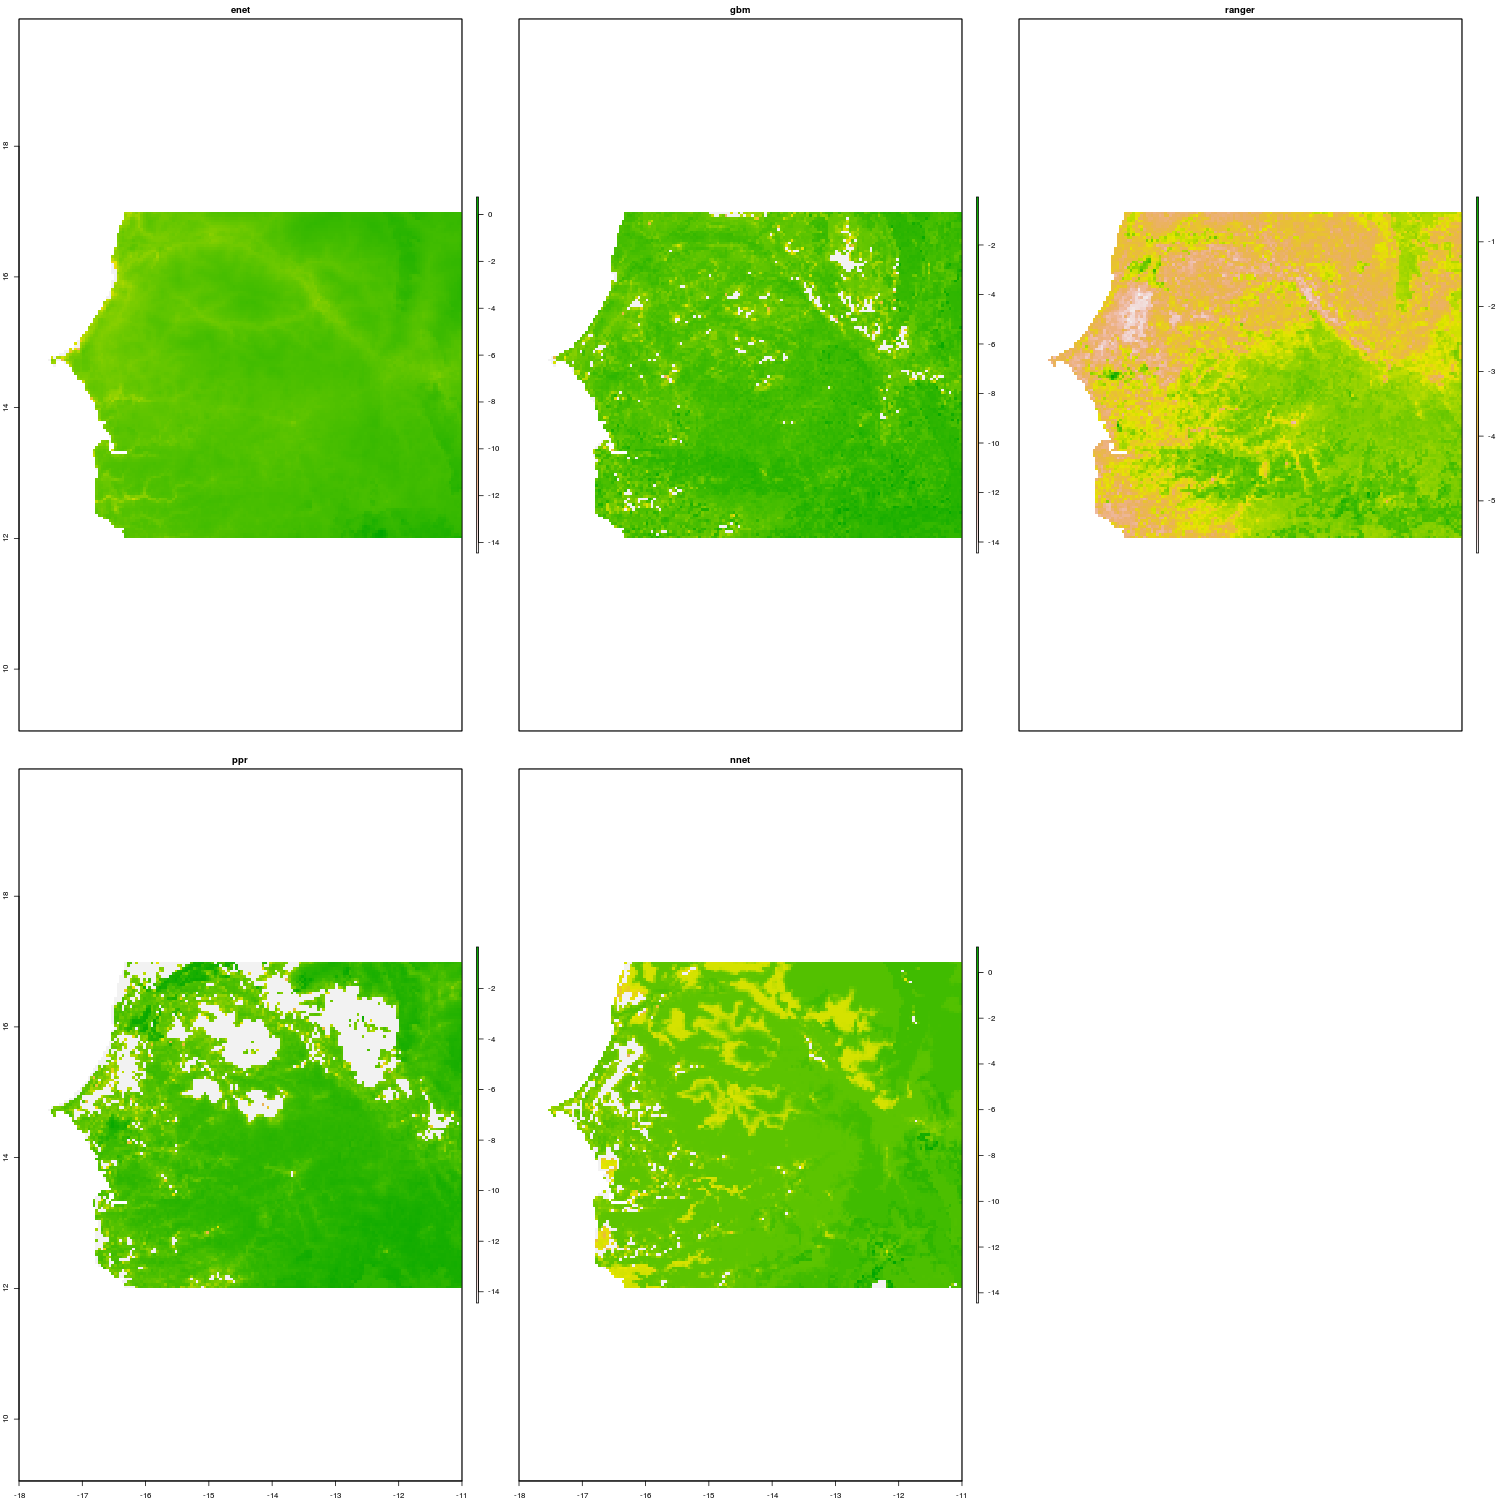
\includegraphics[width=1\textwidth]{figs/SI/sen_all_ml.png}
\caption{
  Predictions from machine learning models trained on Senegal prevalence data.
}

\end{figure}


\begin{figure}[h!]
  \centering
  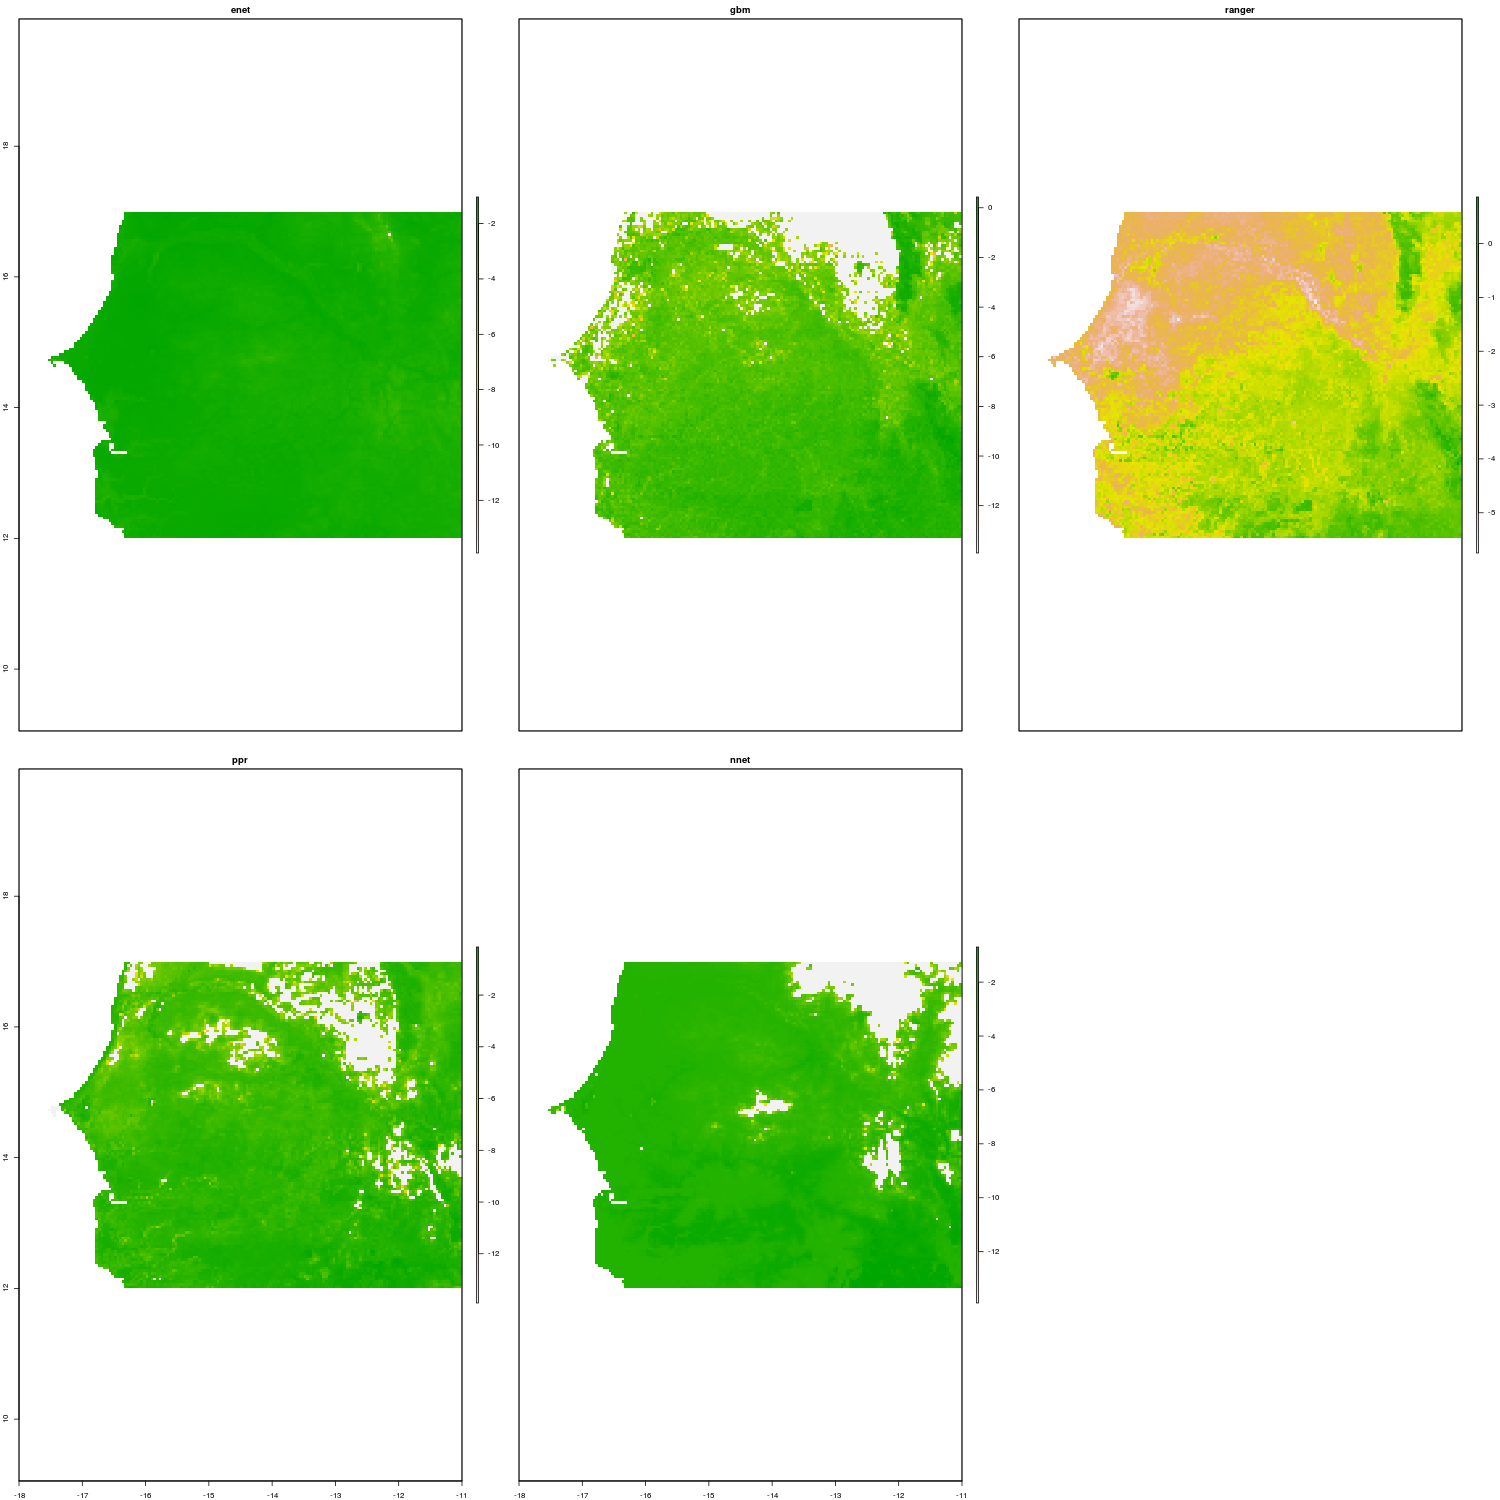
\includegraphics[width=1\textwidth]{figs/SI/sen_all_globalml.png}
\caption{
  Predictions from machine learning models trained on Senegal prevalence data.
}

\end{figure}



\clearpage
\subsection{Out-of-sample scatter plots}


\begin{figure}[h!]
  \centering
  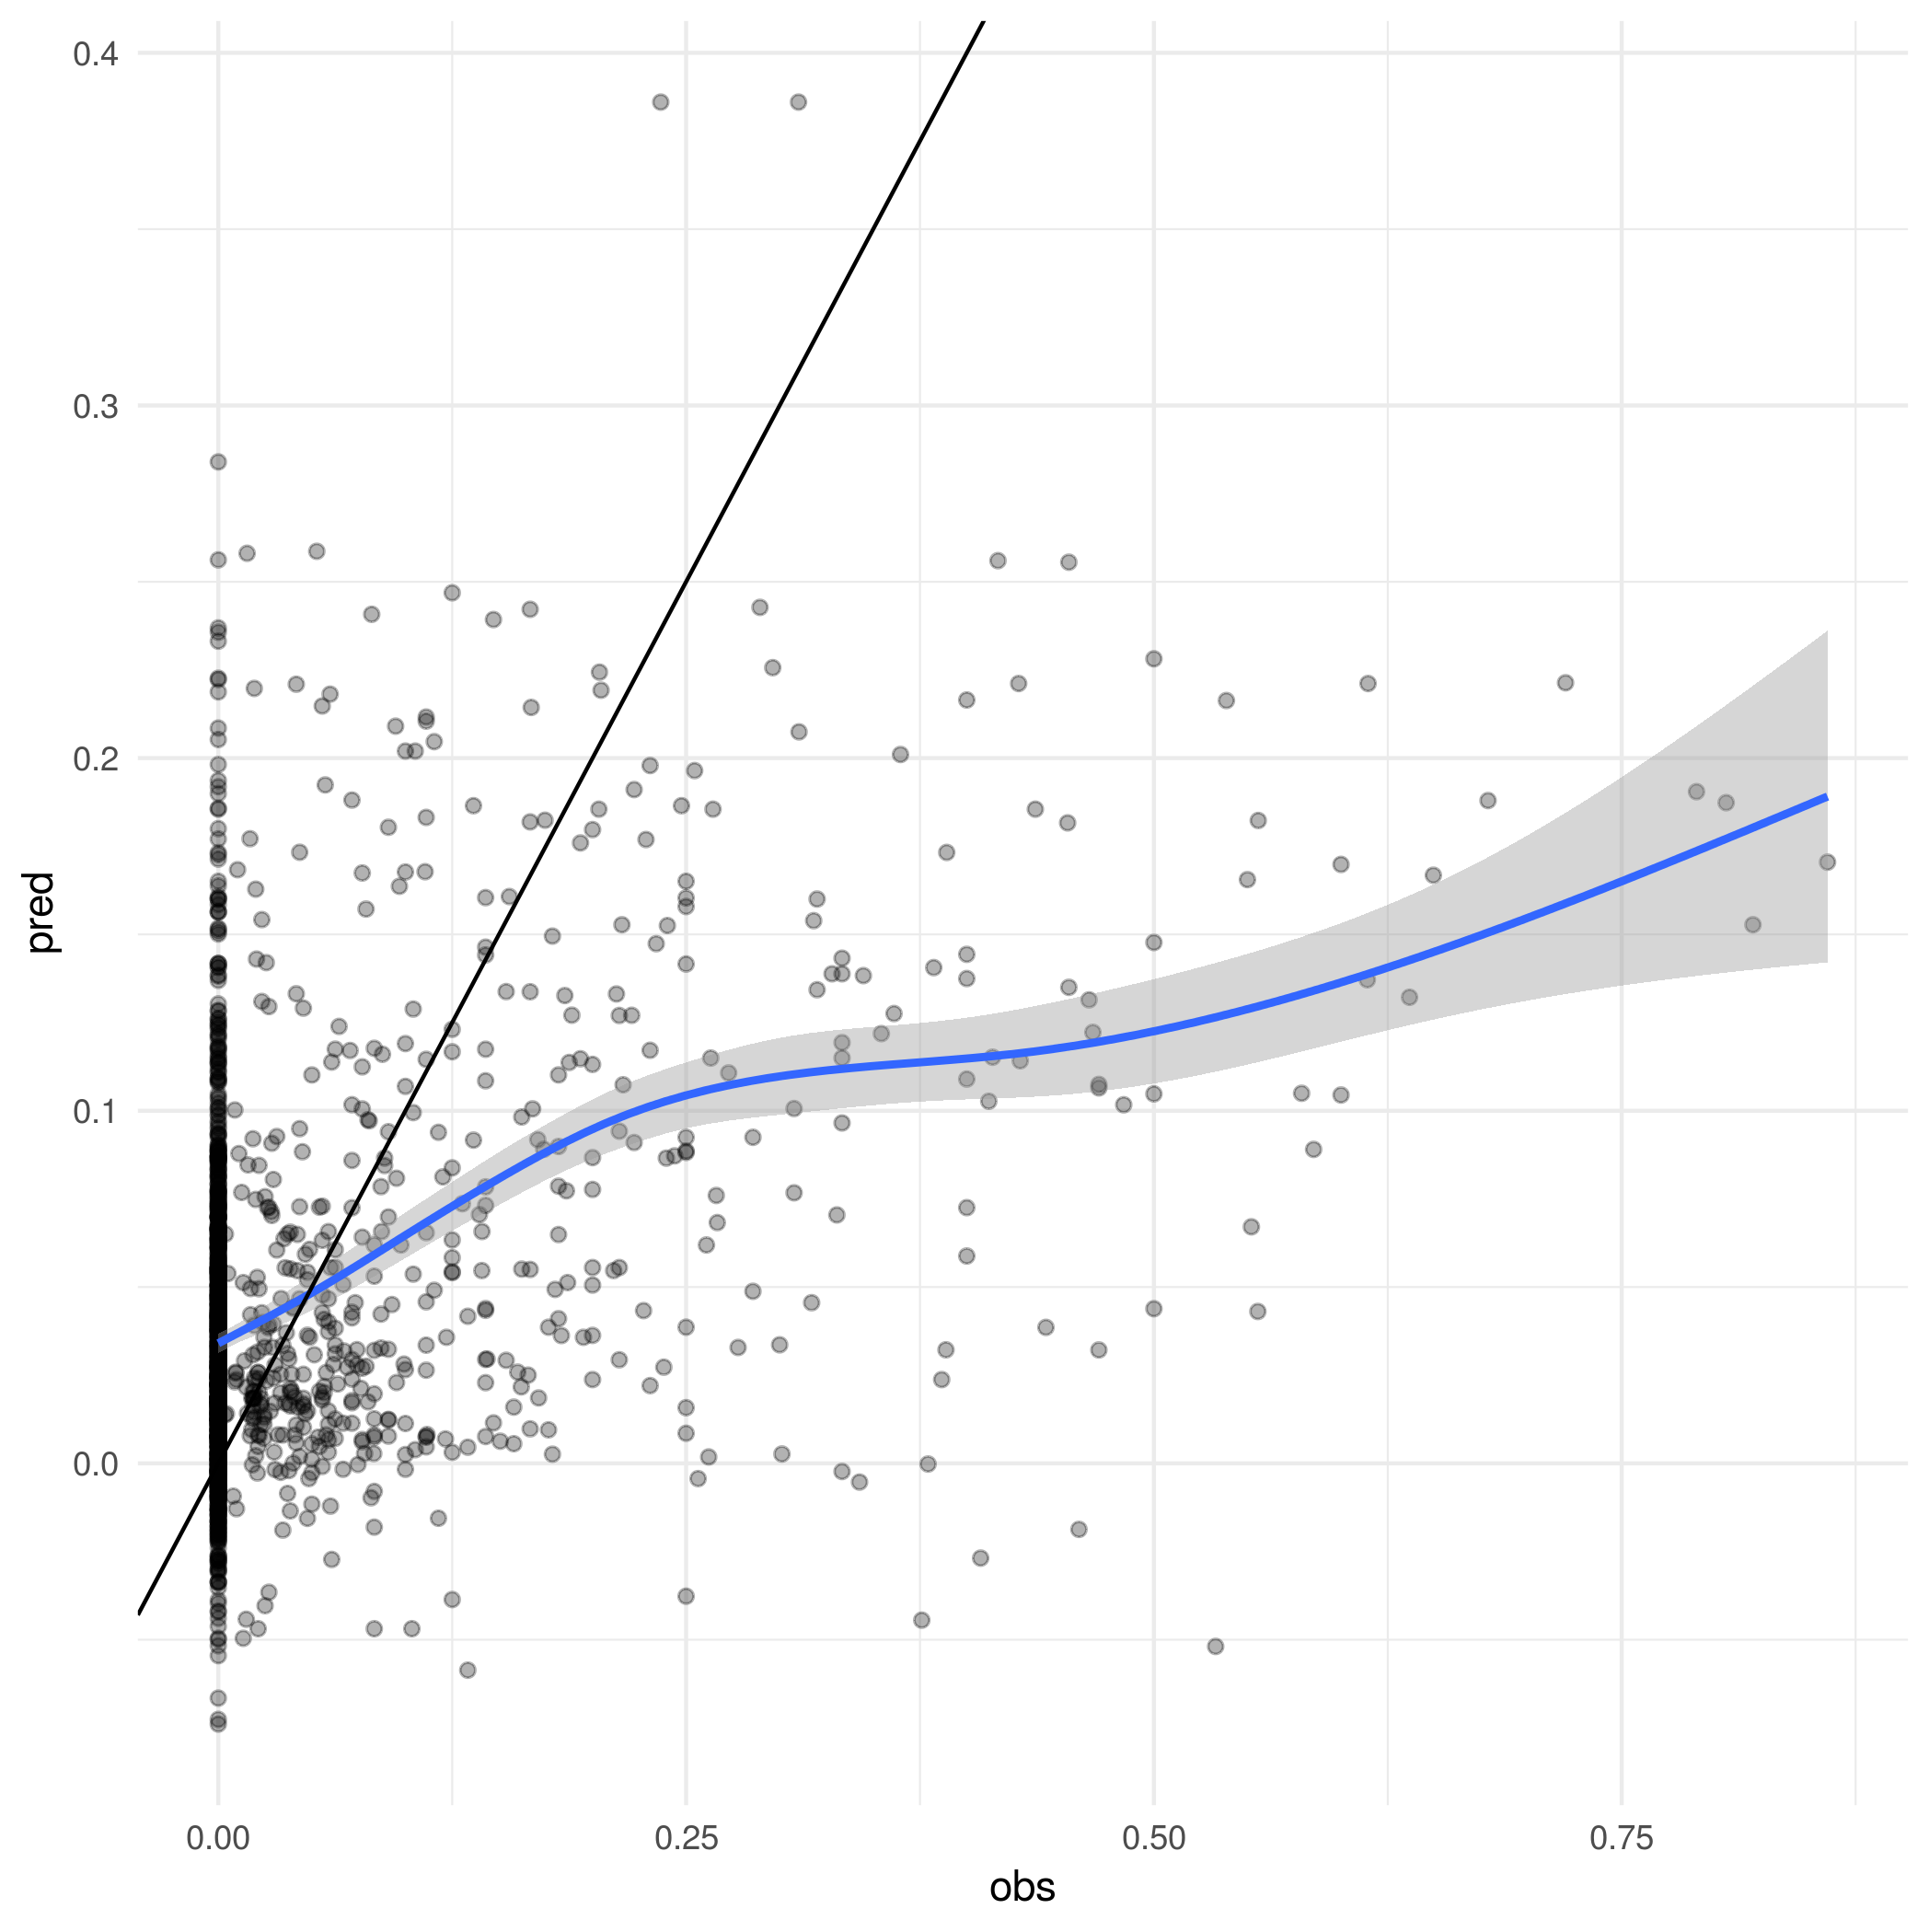
\includegraphics[width=0.6\textwidth]{figs/SI/nnet_obspred_sen.png}
\caption{
  Scatter plot of predictions and held out observed data for the neural network trained on the Senegal dataset.
}

\end{figure}



\begin{figure}[h!]
  \centering
  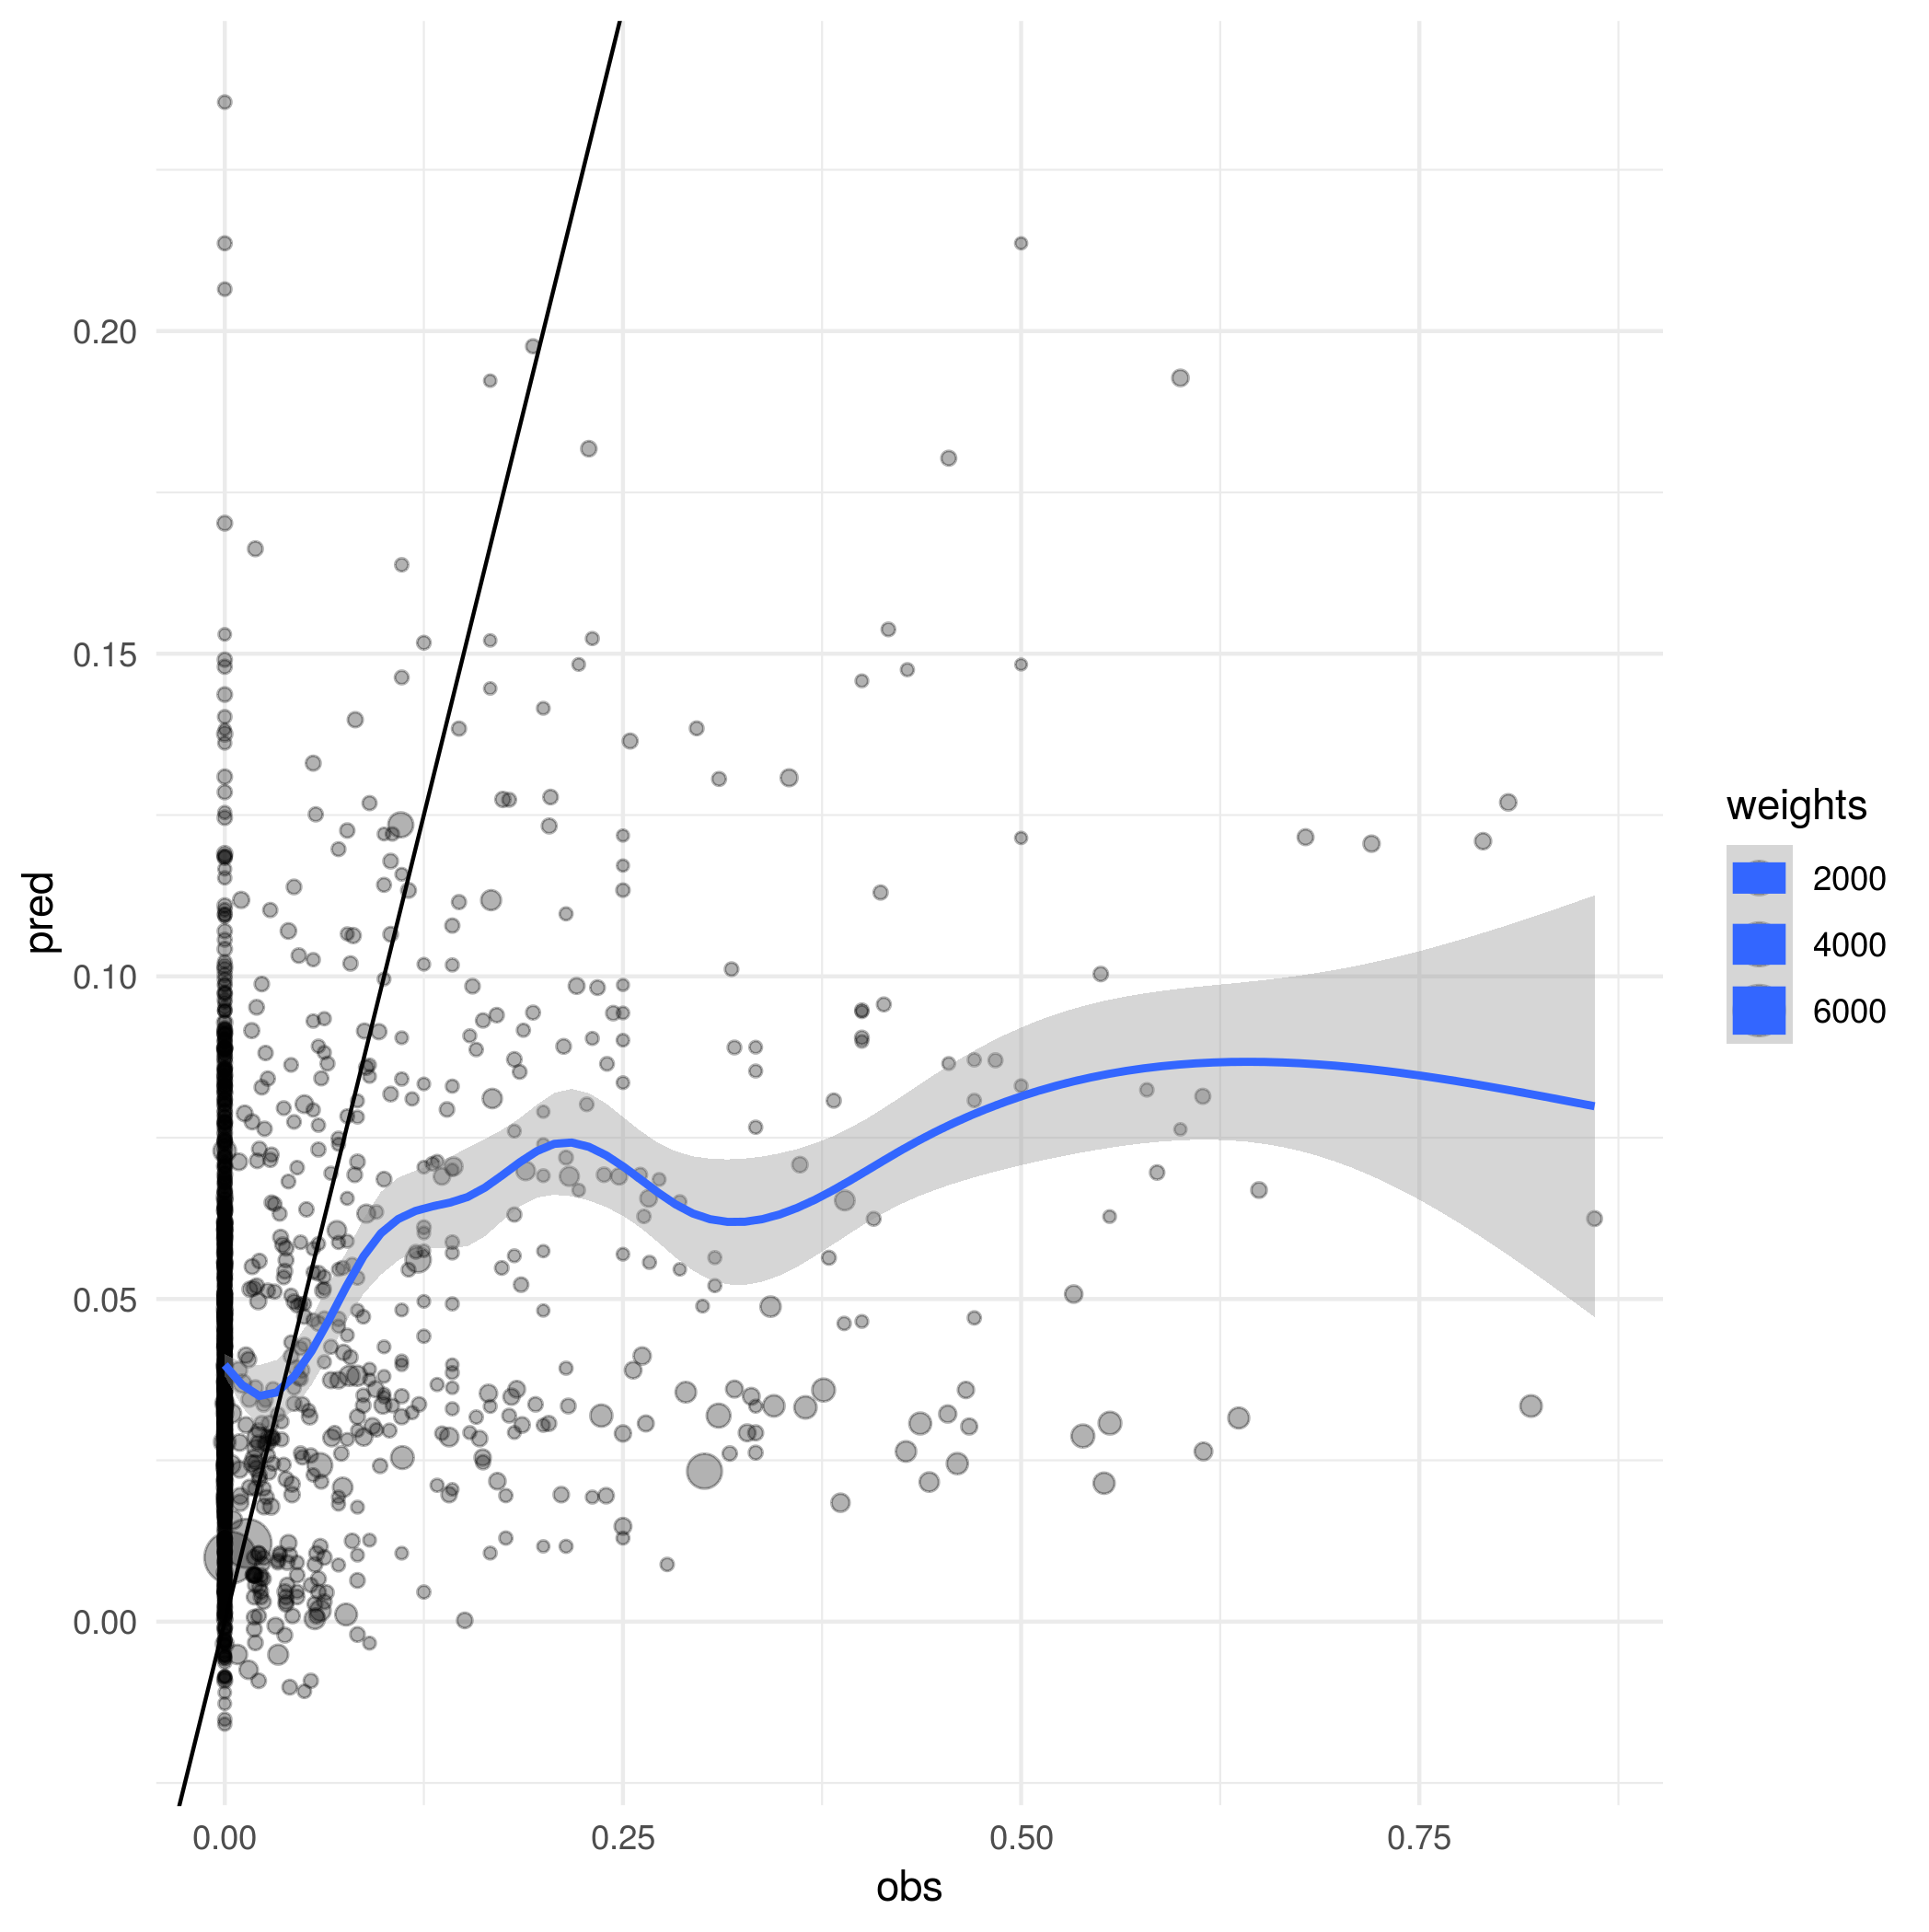
\includegraphics[width=0.6\textwidth]{figs/SI/enet_obspred_sen.png}
\caption{
  Scatter plot of predictions and held out observed data for the elastic net trained on the Senegal dataset.
}

\end{figure}


\begin{figure}[h!]
  \centering
  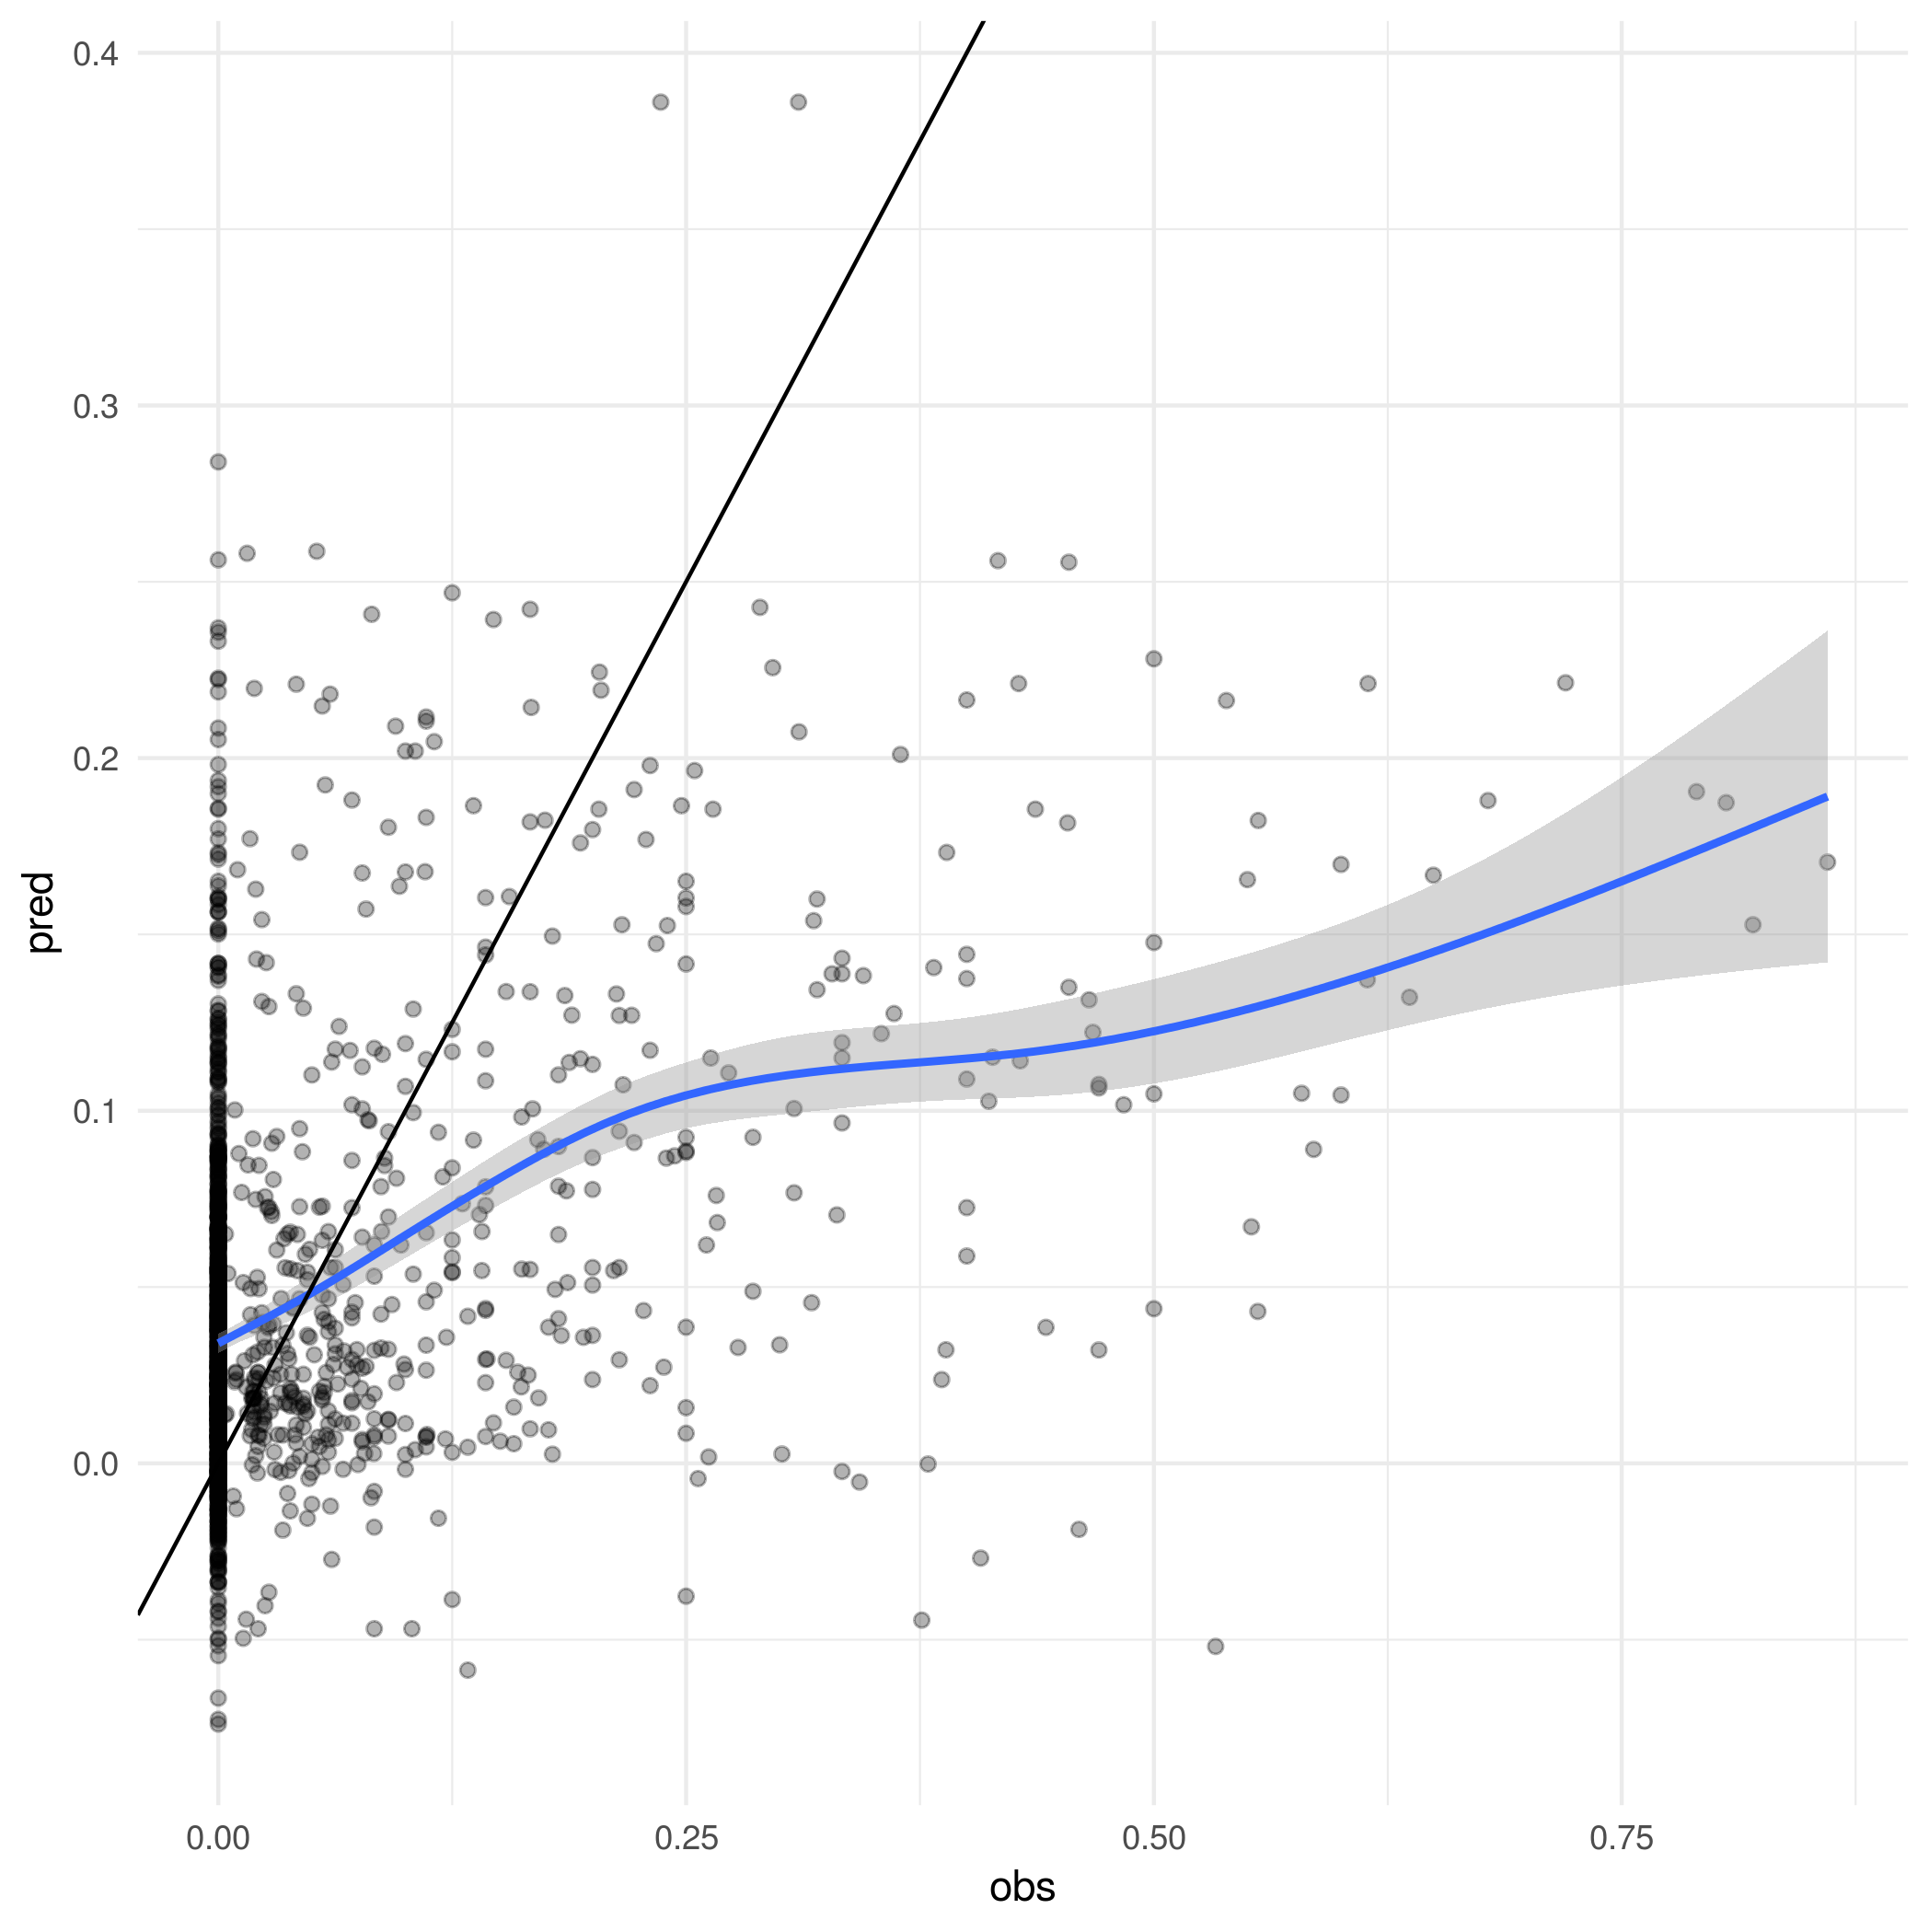
\includegraphics[width=0.6\textwidth]{figs/SI/ppr_obspred_sen.png}
\caption{
  Scatter plot of predictions and held out observed data for the PPR trained on the Senegal dataset.
}

\end{figure}


\begin{figure}[h!]
  \centering
  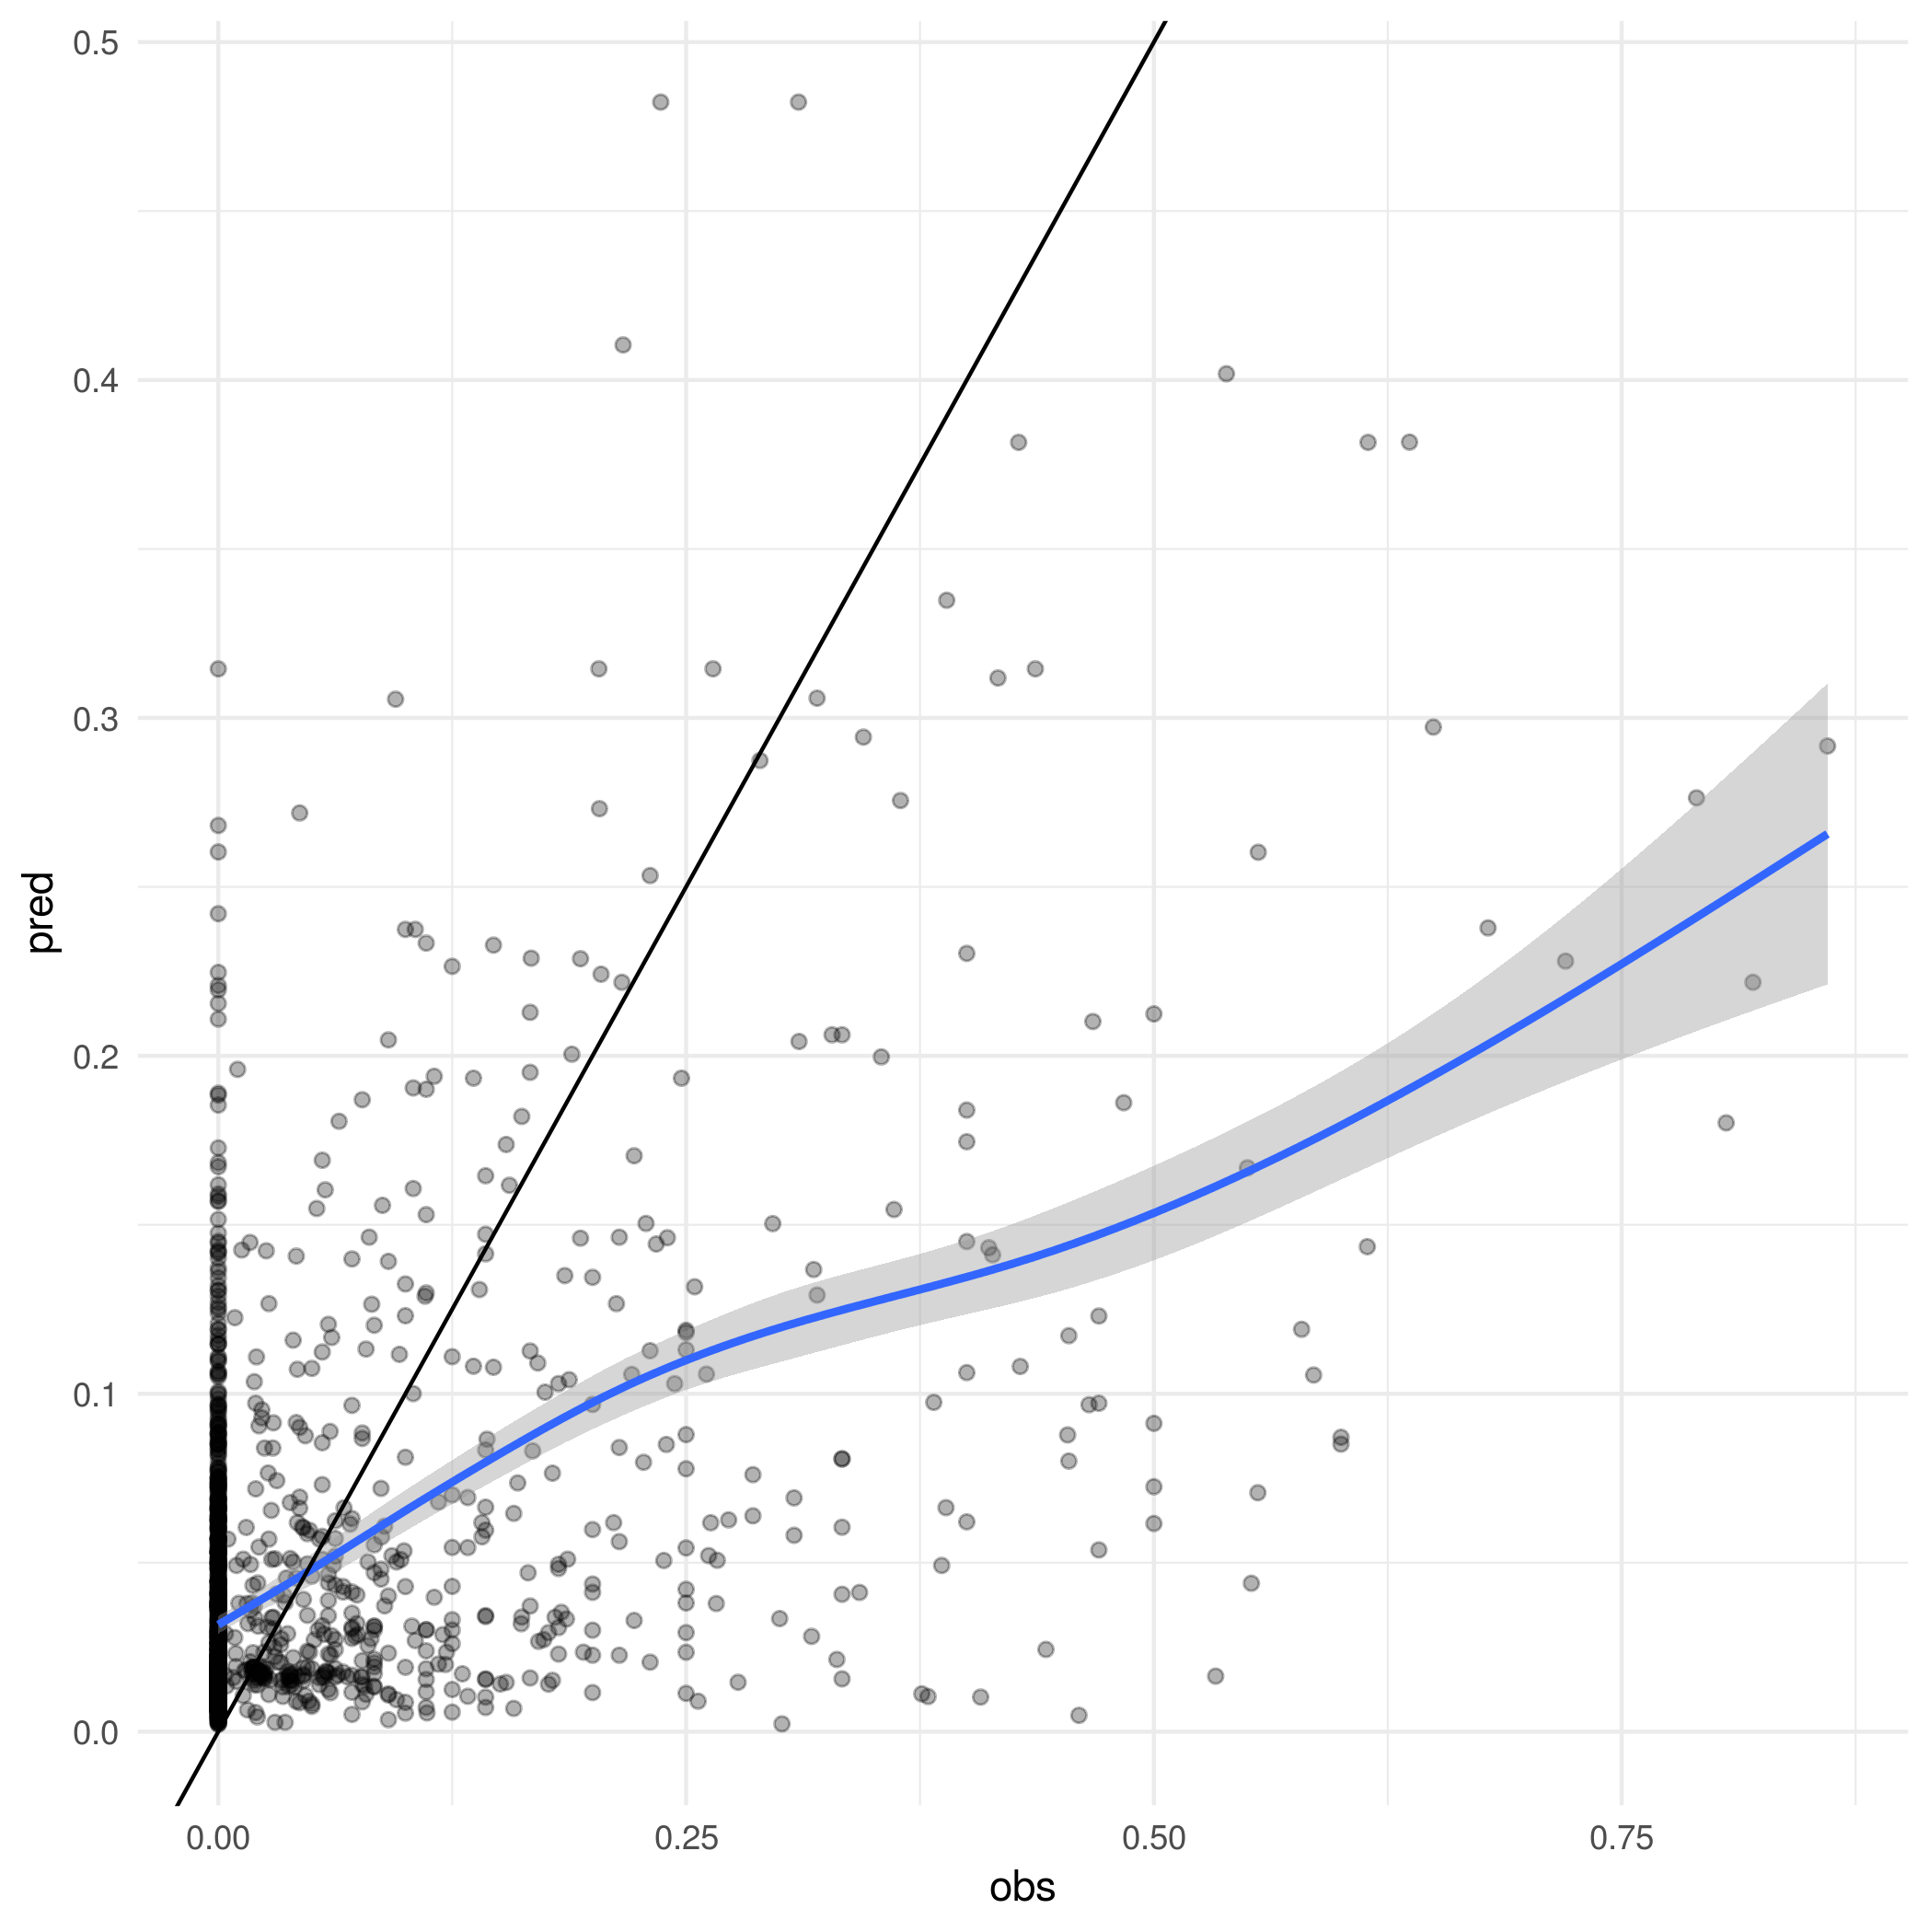
\includegraphics[width=0.6\textwidth]{figs/SI/ranger_obspred_sen.png}
\caption{
  Scatter plot of predictions and held out observed data for the Random Forest trained on the Senegal dataset.
}

\end{figure}


\begin{figure}[h!]
  \centering
  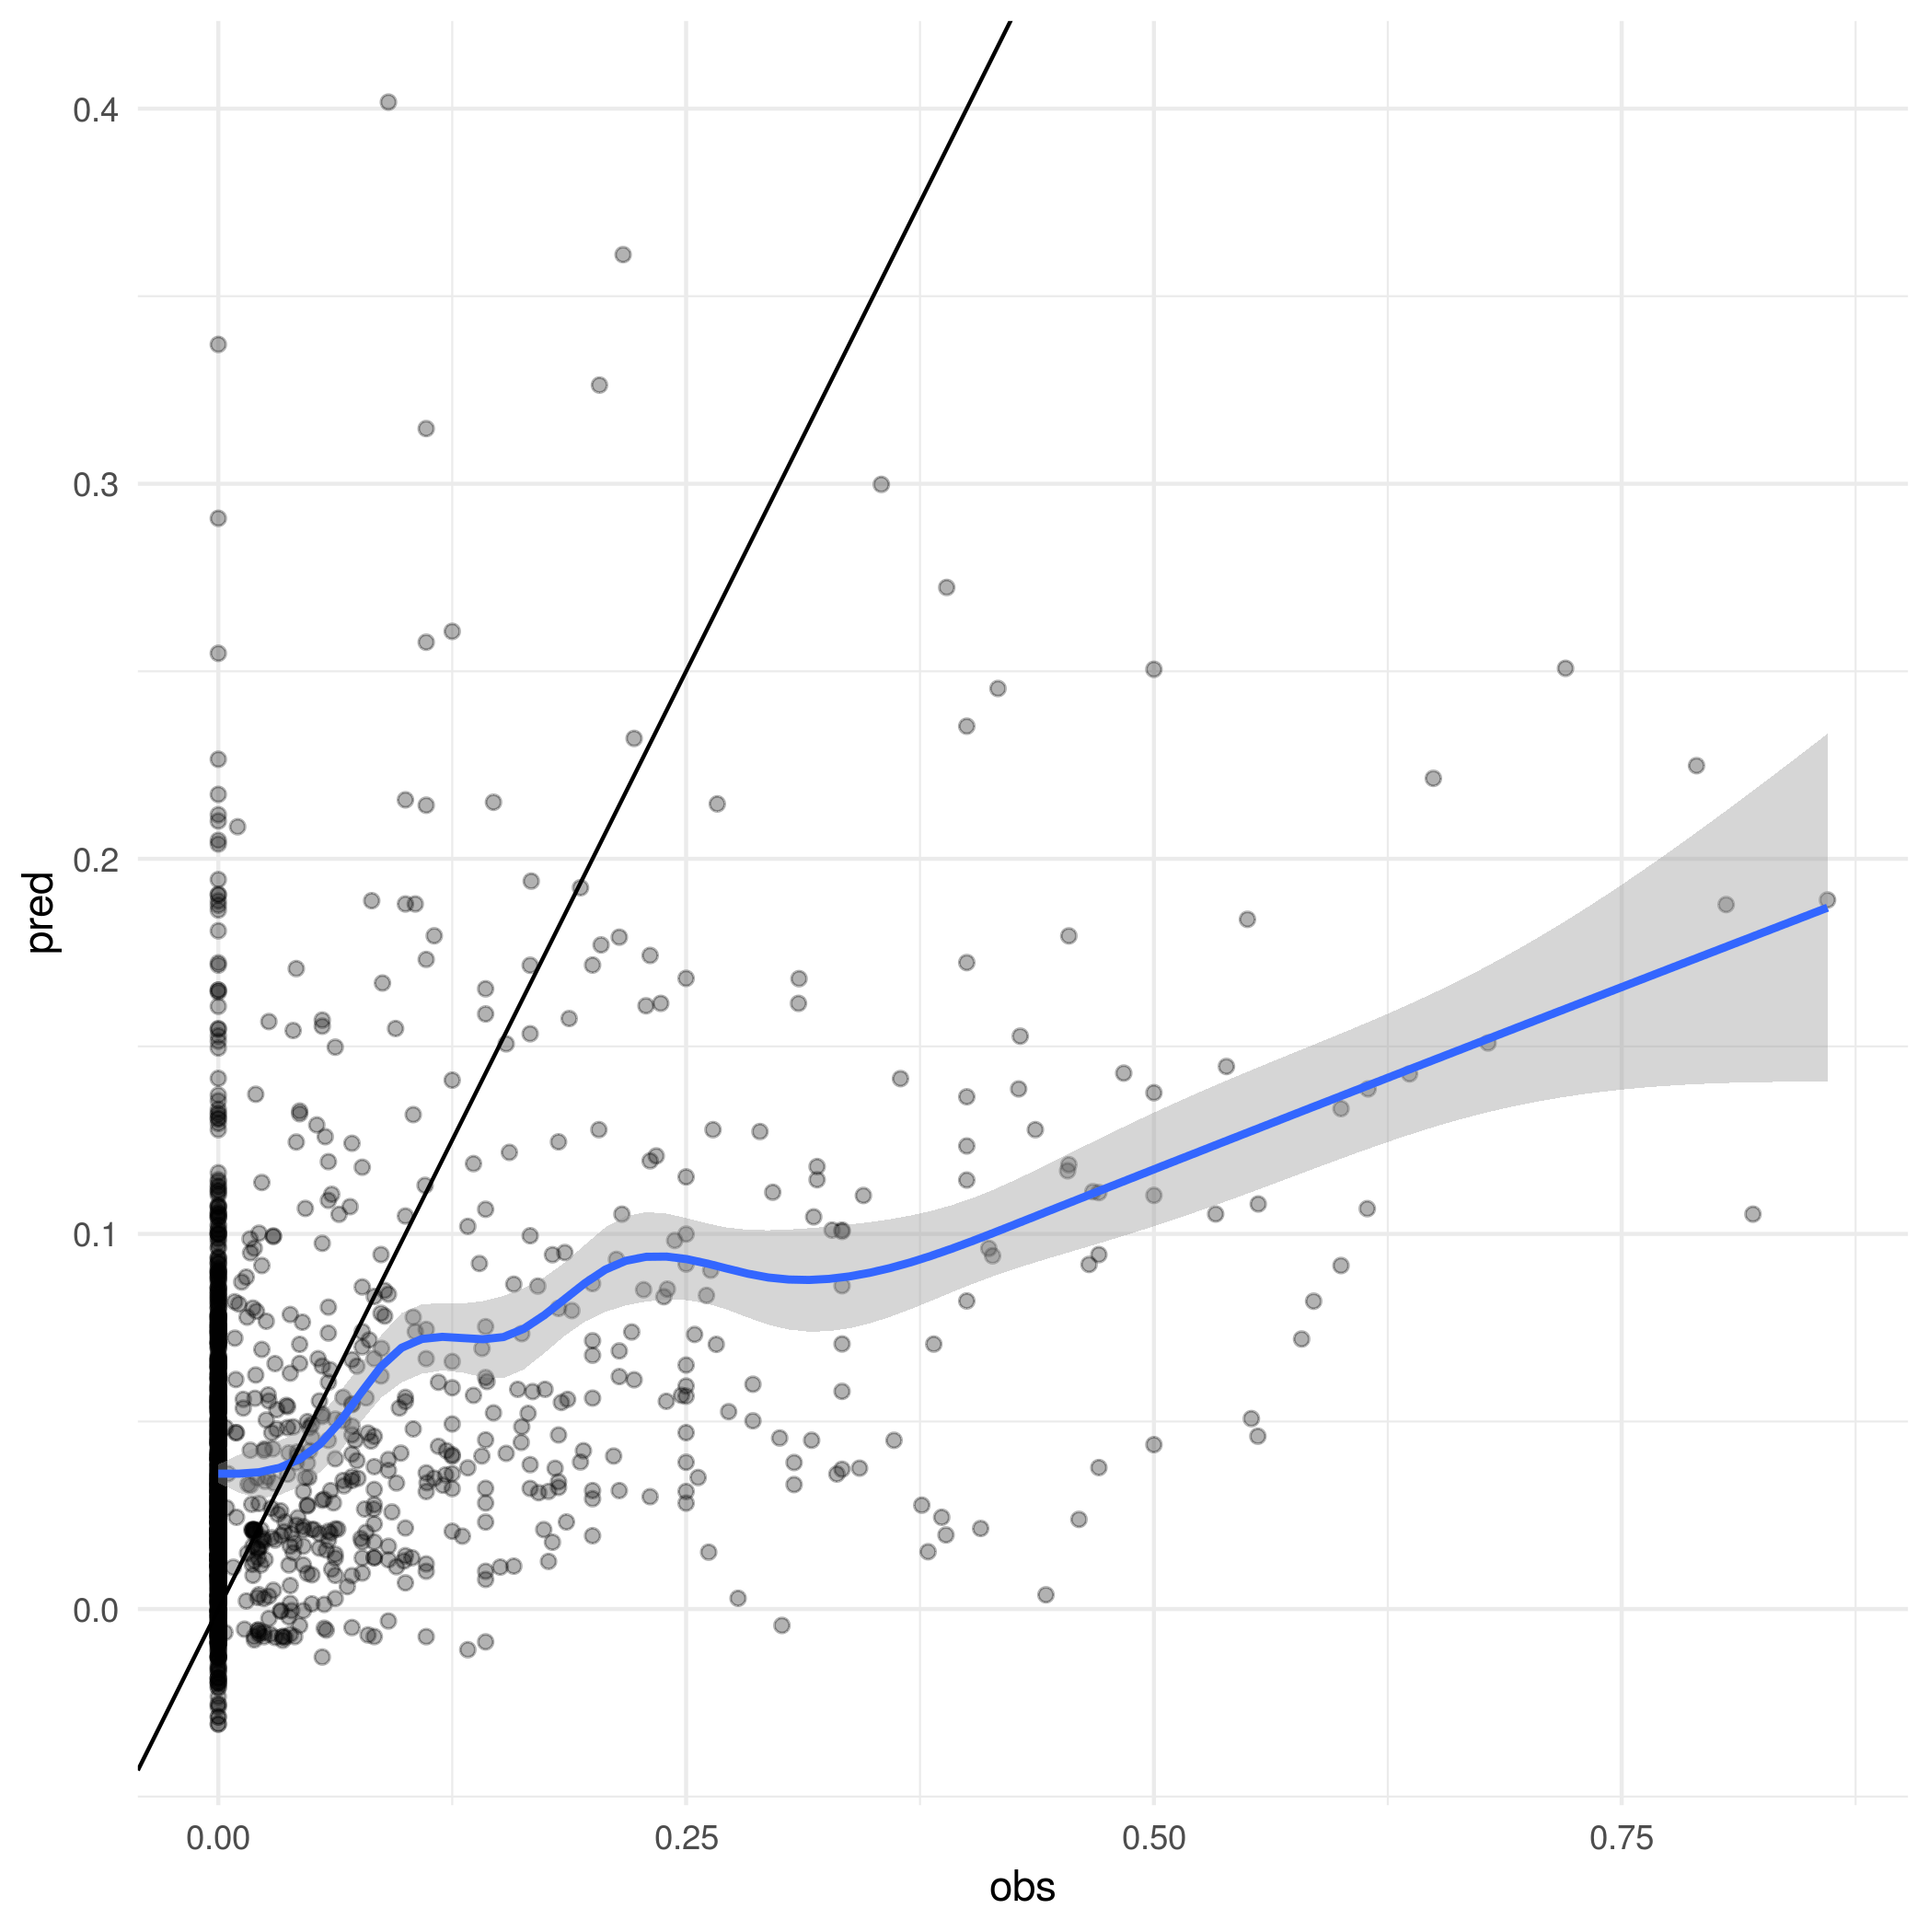
\includegraphics[width=0.6\textwidth]{figs/SI/xgboost_obspred_sen.png}
\caption{
  Scatter plot of predictions and held out observed data for the GBM trained on the Senegal dataset.
}

\end{figure}


\clearpage
\subsection{Hyperparameter optimisation}

As ranger and GBM were tuned with random hyperparameter search, the plots become difficult and are not included.


\begin{figure}[h!]
  \centering
  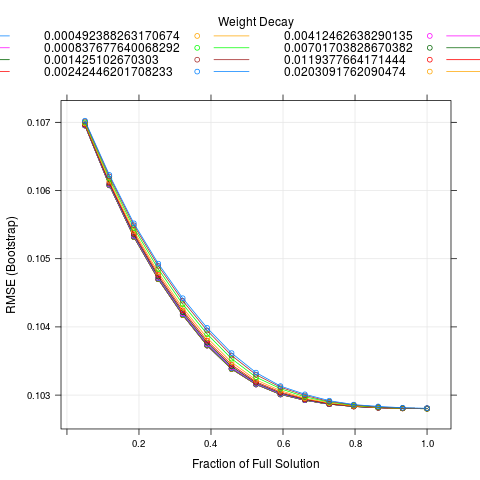
\includegraphics[width=0.6\textwidth]{figs/SI/enetopt_sen.png}
\caption{
  Optimisation for elastic net hyperparameters trained on the Senegal dataset.
}
\end{figure}



\begin{figure}[h!]
  \centering
  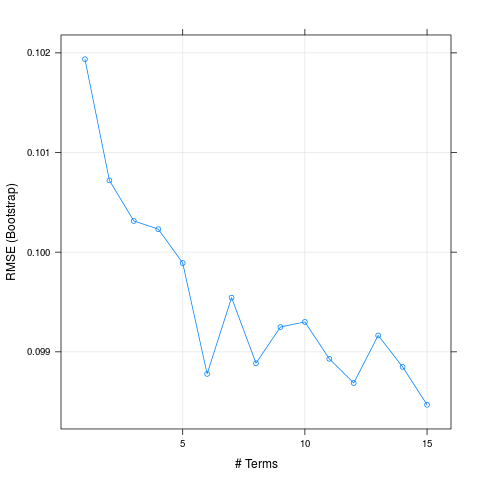
\includegraphics[width=0.6\textwidth]{figs/SI/ppropt_sen.png}
\caption{
  Optimisation for PPR hyperparameters trained on the Senegal dataset.
}

\end{figure}



%\section*{Citations}
%\bibliography{Malaria} 
%\bibliographystyle{unsrt}
%\bibliographystyle{apalike}




\end{document}









